% Options for packages loaded elsewhere
\PassOptionsToPackage{unicode}{hyperref}
\PassOptionsToPackage{hyphens}{url}
%
\documentclass[
]{book}
\usepackage{amsmath,amssymb}
\usepackage{iftex}
\ifPDFTeX
  \usepackage[T1]{fontenc}
  \usepackage[utf8]{inputenc}
  \usepackage{textcomp} % provide euro and other symbols
\else % if luatex or xetex
  \usepackage{unicode-math} % this also loads fontspec
  \defaultfontfeatures{Scale=MatchLowercase}
  \defaultfontfeatures[\rmfamily]{Ligatures=TeX,Scale=1}
\fi
\usepackage{lmodern}
\ifPDFTeX\else
  % xetex/luatex font selection
\fi
% Use upquote if available, for straight quotes in verbatim environments
\IfFileExists{upquote.sty}{\usepackage{upquote}}{}
\IfFileExists{microtype.sty}{% use microtype if available
  \usepackage[]{microtype}
  \UseMicrotypeSet[protrusion]{basicmath} % disable protrusion for tt fonts
}{}
\makeatletter
\@ifundefined{KOMAClassName}{% if non-KOMA class
  \IfFileExists{parskip.sty}{%
    \usepackage{parskip}
  }{% else
    \setlength{\parindent}{0pt}
    \setlength{\parskip}{6pt plus 2pt minus 1pt}}
}{% if KOMA class
  \KOMAoptions{parskip=half}}
\makeatother
\usepackage{xcolor}
\usepackage{longtable,booktabs,array}
\usepackage{calc} % for calculating minipage widths
% Correct order of tables after \paragraph or \subparagraph
\usepackage{etoolbox}
\makeatletter
\patchcmd\longtable{\par}{\if@noskipsec\mbox{}\fi\par}{}{}
\makeatother
% Allow footnotes in longtable head/foot
\IfFileExists{footnotehyper.sty}{\usepackage{footnotehyper}}{\usepackage{footnote}}
\makesavenoteenv{longtable}
\usepackage{graphicx}
\makeatletter
\def\maxwidth{\ifdim\Gin@nat@width>\linewidth\linewidth\else\Gin@nat@width\fi}
\def\maxheight{\ifdim\Gin@nat@height>\textheight\textheight\else\Gin@nat@height\fi}
\makeatother
% Scale images if necessary, so that they will not overflow the page
% margins by default, and it is still possible to overwrite the defaults
% using explicit options in \includegraphics[width, height, ...]{}
\setkeys{Gin}{width=\maxwidth,height=\maxheight,keepaspectratio}
% Set default figure placement to htbp
\makeatletter
\def\fps@figure{htbp}
\makeatother
\setlength{\emergencystretch}{3em} % prevent overfull lines
\providecommand{\tightlist}{%
  \setlength{\itemsep}{0pt}\setlength{\parskip}{0pt}}
\setcounter{secnumdepth}{5}
% definitions for citeproc citations
\NewDocumentCommand\citeproctext{}{}
\NewDocumentCommand\citeproc{mm}{%
  \begingroup\def\citeproctext{#2}\cite{#1}\endgroup}
\makeatletter
 % allow citations to break across lines
 \let\@cite@ofmt\@firstofone
 % avoid brackets around text for \cite:
 \def\@biblabel#1{}
 \def\@cite#1#2{{#1\if@tempswa , #2\fi}}
\makeatother
\newlength{\cslhangindent}
\setlength{\cslhangindent}{1.5em}
\newlength{\csllabelwidth}
\setlength{\csllabelwidth}{3em}
\newenvironment{CSLReferences}[2] % #1 hanging-indent, #2 entry-spacing
 {\begin{list}{}{%
  \setlength{\itemindent}{0pt}
  \setlength{\leftmargin}{0pt}
  \setlength{\parsep}{0pt}
  % turn on hanging indent if param 1 is 1
  \ifodd #1
   \setlength{\leftmargin}{\cslhangindent}
   \setlength{\itemindent}{-1\cslhangindent}
  \fi
  % set entry spacing
  \setlength{\itemsep}{#2\baselineskip}}}
 {\end{list}}
\usepackage{calc}
\newcommand{\CSLBlock}[1]{\hfill\break\parbox[t]{\linewidth}{\strut\ignorespaces#1\strut}}
\newcommand{\CSLLeftMargin}[1]{\parbox[t]{\csllabelwidth}{\strut#1\strut}}
\newcommand{\CSLRightInline}[1]{\parbox[t]{\linewidth - \csllabelwidth}{\strut#1\strut}}
\newcommand{\CSLIndent}[1]{\hspace{\cslhangindent}#1}

% Load packages
\usepackage{booktabs}
\usepackage{amsthm}
\usepackage{svg}
\usepackage[english]{babel}
\usepackage{fancyhdr}

% Change "Chapter" to "Kapitel" throughout document
\addto\captionsenglish{\renewcommand{\chaptername}{Kapitel}}
% Change "Content" to "Indholdsfortegnelse"
\addto\captionsenglish{\renewcommand{\contentsname}{Indholdsfortegnelse}}
% Change "Appendix" to "Bilag"
\addto\captionsenglish{\renewcommand{\appendixname}{Bilag}}

% Page layout
\makeatletter
\def\thm@space@setup{%
  \thm@preskip=8pt plus 2pt minus 4pt
  \thm@postskip=\thm@preskip
}
\makeatother
\usepackage{flafter}
\usepackage{booktabs}
\usepackage{caption}
\usepackage{longtable}
\usepackage{colortbl}
\usepackage{array}
\ifLuaTeX
  \usepackage{selnolig}  % disable illegal ligatures
\fi
\usepackage{bookmark}
\IfFileExists{xurl.sty}{\usepackage{xurl}}{} % add URL line breaks if available
\urlstyle{same}
\hypersetup{
  pdftitle={En befolkning blander sig},
  pdfauthor={Lanciné Diop-Christensen, Christian Albrekt Larsen (red.), Jeppe Fjeldgaard Larsen og Hans-Peter Y. Qvist},
  hidelinks,
  pdfcreator={LaTeX via pandoc}}

\title{En befolkning blander sig}
\author{Lanciné Diop-Christensen, Christian Albrekt Larsen (red.), Jeppe Fjeldgaard Larsen og Hans-Peter Y. Qvist}
\date{2024-08-23}

\begin{document}
\maketitle

{
\setcounter{tocdepth}{1}
\tableofcontents
}
\chapter*{\texorpdfstring{Forord (\textbf{WIP DO NOT CITE ANY CONTENT})}{Forord (WIP DO NOT CITE ANY CONTENT)}}\label{forord-wip-do-not-cite-any-content}
\addcontentsline{toc}{chapter}{Forord (\textbf{WIP DO NOT CITE ANY CONTENT})}

Bogen er baseret på forskningsprojektet \emph{''Measuring intense migrant-native contact and its concequences''} (MNcontact), der var finansieret af Den Fri Forskningsfond i perioden fra 2019 til 2024. Bogen er en formidlingsbog, der er baseret på projektets datamateriale og forskningsresultater.

Projektgruppen har bestået af undertegnet, \href{https://vbn.aau.dk/da/persons/jeppefl}{Jeppe Fjeldgaard Larsen}, \href{https://vbn.aau.dk/en/persons/led}{Lanciné Eric Diop-Christensen}, \href{https://vbn.aau.dk/da/persons/hpq}{Hans-Peter Y. Qvist}, \href{https://vbn.aau.dk/en/persons/jy}{Jeevitha Y. Qvist}, \href{https://vbn.aau.dk/en/persons/troelsfh}{Troels Fage Hedegaard} og \href{https://dk.linkedin.com/in/anna-diop-christensen-58b5ba282}{Anna Diop-Christensen} (i tilfældig rækkefølje). Gruppen har i forskellige konstellationer publiceret en række videnskabelige publikationer og flere er på vej. De er samlet på \href{https://www.politics-society.aau.dk/research/projects/mncontact}{projektets hjemmeside}.

Undervejs har vi arbejdet tæt sammen \href{https://vbn.aau.dk/en/persons/anbajo}{Anders Bastrup Jørgensen}, der skrev Ph.D-afhandling om indvandrere og efterkommeres deltagelse i frivillige foreninger. Vi har også arbejdet sammen med \href{https://vbn.aau.dk/en/persons/rolfll}{Rolf Lyneborg Lund} og \href{https://vbn.aau.dk/en/persons/anjaj}{Anja Jørgensen}, der i samme periode analyserede spørgsmålet om indvandrere- og efterkommeres boligmæssige placering.

Vi ønsker alle en god læselyst

Aalborg 2024

\href{https://vbn.aau.dk/en/persons/albrekt}{Christian Albrekt Larsen}

Forskningsleder på MNcontact.\\
Professor, Institut for Politik og Samfund\\
Aalborg Universitet\\

ISSN: xxxx-xxxx\\
ISBN: xxx-xx-xxxx-xxx-x

Published by:\\
Aalborg University Press\\
Skjernvej 4A, 2nd floor\\
DK -- 9220 Aalborg Ø\\
Phone: +45 99407140\\
\href{mailto:aauf@forlag.aau.dk}{\nolinkurl{aauf@forlag.aau.dk}}\\
forlag.aau.dk

© Copyright by author

\chapter{En befolkning blander sig}\label{kap1}

\emph{\href{https://vbn.aau.dk/en/persons/albrekt}{Christian Albrekt Larsen}}


\includegraphics[width=1\linewidth]{images/dalle-smeltedige}

Denne bog bygger på to centrale antagelser. For det første, at tilstedeværelsen af sociale relationer og tillidsbånd på tværs af etniske grupper er afgørende for at sikre et velfungerende og trygt samfund. For det andet, at disse sociale relationer og tillidsbånd primært opstår, når mennesker mødes ansigt-til-ansigt i forskellige sammenhænge fx i familier, skoler og på arbejdspladser. Med det udgangspunkt fokuserer denne bog på forudsætningerne for, at der kan dannes sociale relationer og tillidsbånd mellem personer med dansk oprindelse og indvandrere og efterkommere i Danmark. Det har vi gjort ved at se nærmere på i hvilket omfang indvandrere og efterkommere og personer med dansk oprindelse er blandede med hinanden i familier og på skoler og arbejdspladser. Derudover har vi også undersøgt om der faktisk dannes sociale relationer mellem indvandrere og deres efterkommere og personer med dansk oprindelse i form af venskaber og parforhold.

Både danskerne og indvandrerne kan påvirkes af at mødes fysisk. Specielt nytilkomne indvandrere har ofte meget at vinde ved at mødes med majoritetsbefolkningen. Det kan blandt andet give nytilkomne information om, hvordan man klarer sig i det nye land. Det klassiske eksempel på såkaldte netværkseffekter stammer fra arbejdsmarkedet, hvor majoritetsbefolkningen ofte har privilegeret information om mulige jobåbninger. Men fysiske møder med majoritetsbefolkningen kan give meget andet relevant information på arbejdsmarkedet. Det kan være alt fra, hvordan pantsystemet og NemID fungerer, til, hvad der er acceptabelt og ikke-acceptabelt at gøre ved en børnefødselsdag. Alle, der har prøvet af bosætte sig i et andet land, ved, at antallet af praktiske spørgsmål nærmest er uendeligt. Mødet med majoritetsbefolkningen er også en mulighed for at få sprogkundskaber. Sproget er som en dåseåbner til et samfund. Det letter adgangen fra den mest specifikke information, fx om det med pantsystemet, til den mest abstrakte information, fx om, hvad danskerne mener en nation er. Sprogkundskaber er også vigtige for at kunne tale sin sag, fx i sundsvæsenet, for at kunne blive accepteret af de andre forældre i ens børns klasse og for at klare sig i uddannelsessystemet. Endeligt kan fysiske møder med majoritetsbefolkningen være en lejlighed få justeret eventuelle negative forestillingerne om, hvordan danskerne er. Indvandrere og efterkommere er ligesom alle andre mennesker. Vi tenderer til at lave positive historier om os selv og negative historier om de andre. Er alle danskere kommet i racisme-kassen, kan ansigt-til-ansigt møder potentielt skabe nuancering.

Majoritetsbefolkningen har typisk ikke helt så meget at vinde ved at mødes ansigt til ansigt med indvandrere. Majoritetsbefolkningen sidder ikke med den samme bunke spørgsmål om, hvordan man klarer og gebærder sig i Danmark. Ønsker majoritetsbefolkningen sig dog ud i verden, kan indvandrere være en kilde til information og sprog. Specielt minoriteten af vellønnede internationale specialister kan have et netværk, som danskerne kan gøre brug af på det internationale arbejdsmarked. Ellers handler det mere om luksusproblemer, som kulturel adspredelse, bedre mad og måske adgang til billig arbejdskraft. Hos majoritetsbefolkningen kan ansigt-til-ansigt møder også være afgørende lejligheder til få justeret eventuelle negative forestillinger om, hvordan indvandrere og efterkommere er. Er alle indvandrere kommet i terrorist-kassen, kan ansigt-til-ansigt møder potentielt også skabe nuancering hos majoritetsbefolkningen.

Møder mellem mennesker kan give grobund for mere eller mindre intime sociale relationer. I den ene ende af skalaen er der overfladiske sociale relationer, hvor vi interagerer uden at ''investere'' nævneværdigt i hinanden. Det kan være flygtige forhold ved køb og salg af varer. I den anden ende af skalaen er der dybe sociale relationer, hvor vi lægger vores liv i hinandens hænder. Det typiske eksempel er indgåelse af ægteskab. Imellem disse ekstremer ligger venskaber. Disse halv intime sociale relationer er interessante, da de formentligt er stærke nok til at ændre på vores forståelser af andre grupper, og formentligt er svage nok til, at vi tør mødes med nogle, der ikke ligner os selv. De er også interessante, da ét menneske kan have mange venskaber, dvs. der er stort potentiale for et højt antal sociale relationer mellem danskere, indvandrere og efterkommere I modsætning til ægteskabs- og samlivsrelationer, hvor der typiske kun etableres én relation per menneske (ad gangen).

I resten af dette kapitel uddyber vi bogens perspektiv. I det første afsnit redegøres for vores forståelse af integration som en dynamisk tovejsproces, der på sigt mindsker betydningen af etniske skel i befolkninger. I det efterfølgende afsnit forklarer vi, hvorfor bogen fokuserer på det vi kalder tvungne mødepladser, dvs. arenaer, hvor der er begrænset mulighed for at fravælge mødet med ''de andre''. I vores optik er disse mødepladser centrale for at bryde en almenmenneskelig tendens til at danne sociale relationer med mennesker, der ligner os selv. I tredje afsnit introducerer vi den socialpsykologiske litteratur, der har beskæftiget med, hvordan ansigt-til-ansigt møder potentielt reducerer betydningen af etniske distinktioner. Efter dette fokus på mikro-mekanismer, vender vi blikket med de makro-mekanismer, der knytter sig til størrelsesforholdene mellem indvandrere, efterkommere og danskere. Den simple pointe er, at gruppestørrelser er afgørende for omfanget af ansigt-til-ansigt møder. Kapitlet afsluttes med en beskrivelse af, hvordan Danmark adskiller fra den amerikanske kontekst, hvor de fleste teorier om integration og assimilering er blevet udviklet, samt en kort refleksion over bogens plan, styrker og begrænsninger.

\section{Integration og assimilering---en tovejsproces}\label{integration-og-assimileringen-tovejsproces}

Bogen er inspireret af den amerikanske forskning i indvandrere og majoritetsbefolkning. Det moderne USA er grundlagt af indvandrere og landet har forsat det største antal udenlandskfødte indbyggere i verden. Amerikanske sociologer har helt siden disciplinens grundlæggelse været optaget af at beskrive, hvordan disse nytilkomne indbyggere blev integreret og hvordan det langsomt forandrede majoritetsbefolkningen. Et af de klassiske eksempler er, hvordan fattige katolske italienske indvandrere i begyndelsen af det 20. århundrede blev opfattet som en uønsket kulturelt distinkt underklasse, i stil med danskernes syn på muslimske indvandrere fra MENAPT-lande, mens de i dag, 100 år senere, opfattes som en del af den nuværende amerikanske hvide kristne majoritet.

Den amerikanske forskning bruger primært termen \emph{assimilering} til at beskrive disse processer, mens europæiske forskere bruger termen \emph{integration}. Den forskellige sprogbrug er dog blot nuancer i forståelsen af det samme fænomen. I begge forståelser handler det om at beskrive og betegne en proces, hvor både indvandrere og majoritet undergår forandringer, der leder til en ny tilstand. Bogen følger Alba og Nee, der definerer assimilation/integration ''som nedgang i betydning af en etnisk distinktion og dens forbundne kulturelle og sociale forskelle. Hvor ''nedgang'' fortolkes således, at den etniske distinktion fremtræder mindre og aftager i relevans for færre og færre domæner af det sociale liv'' (\citeproc{ref-alba1997}{1997}: 863, egen oversættelse).

Betydningen af en etnisk distinktion reduceres i et gensidigt spil mellem indvandrere og majoritetsbefolkningen. En etnisk skillelinje kan for eksempel udviskes ved, at nogle indvandrere krydser grænsen og definerer sig selv som majoritetsbefolkning. Man kan frasige sig sin oprindelige kultur og indoptage den nye. Det er sådan hverdagssproget beskriver assimilering på individniveau. Men betydningen af en etnisk skillelinje kan også reduceres ved, at grænsen mellem de to grupper gøres mindre tydelig. Et eksempel er, at danskerne tillægger kristendom mindre og mindre betydning for at være dansk; specielt de yngre generationer (\citeproc{ref-larsen2016}{C. A. Larsen, 2016}). Det er med til at udviske skillelinjen mellem den kristne majoritet og de ofte ikke-kristne indvandrere. På samme måde som betydningen af forskellen mellem katolsk og protestantisk blev reduceret i USA. Tilbage står en bredere forståelse af, hvad det vil sige at være dansk eller amerikansk.

Vores perspektiv er, at integration/assimilation som hovedregel \emph{ikke} er noget majoritetsbefolkninger og indvandrere vælger eller fravælger. Integration/assimilation er snarere et biprodukt af levede liv, der har handlet om alt muligt andet. Ønsket om kærlighed via parhold og ægteskab er det klassiske eksempel. Børnene fra parhold mellem majoritetsbefolkning og indvandrere udvisker og udvider eksisterende etniske skillelinjer, selvom det ikke være planlagt. Derfor har den amerikanske forskning ofte brugt antallet af giftemål mellem befolkningsgrupper, som en vigtig indikator på graden af integration. Derfor starter denne bog også med basale demografiske beskrivelser og etablering af en ny klassifikation, der kan beskrive antallet af børn fra ''blandede'' forhold.

En anden grundlæggende drivkraft er jagten på økonomiske ressourcer. I en markedsøkonomi er hovedparten af både majoritetsbefolkningen og indvandrere nødsaget til at sælge deres arbejdskraft for at skaffe økonomiske ressourcer. Det gælder i særdeleshed for indvandrerne, da de typisk ankommer i den arbejdsdygtige alder og typisk har dårligere adgang til overførselsindkomster end majoritetsbefolkningen. Indvandrere besætter typisk lavere lønnede jobs i mindre regulerede sektorer, men de vil have et betydeligt incitament til at søge jobs i mere velbetalte sektorer, hvor majoritetsbefolkningen dominerer. Indvandrere har også et betydeligt incitament til at investere i uddannelsesbeviser fra destinationslandet, da disse ofte fungerer som adgangsbillet til attraktive stillinger. Både i uddannelsessektoren og på arbejdsmarkedet møder indvandrerne og danskerne hinanden, men det ikke derfor, at de er der. Integration er således typisk et biprodukt. Kunne man helt selv bestemme, hvem man gerne ville interagere med, så havde vi formentligt et langt mere opdelt samfund.

\section{Drivkraften mod sine egne og tvungne mødepladser}\label{drivkraften-mod-sine-egne-og-tvungne-muxf8depladser}

En etnisk distinktion skal have betydning før, at den kan miste sin betydning. Med en verden opdelt i nationalstater, der både afspejler etniske grupperinger og aktivt understøtter nationale sprog og kulturer, kan etniske distinktioner nærmest tages for givet. Italienerne ankom til USA med en forståelse af, at de var italienere. Og amerikanerne opfattede de nyankomne, som italienere. På samme måde som polakker og syrere ankommer til Danmark med en forståelse af, at de er polske eller syriske. Ligeledes oplever danskerne, at det netop er polakker og syrer, der ankommer. Samtidigt ligger det dybt i mennesket natur, at vi gerne vil være sammen med andre mennesker, der ligner os selv. Det skyldes formentligt en søgen efter anerkendelse og beskyttelse i en gruppe. Det er vist i et utal af sociologiske undersøgelser, at vi primært etablerer venskaber og partnerskaber med nogle, der ligner os selv (\citeproc{ref-mcpherson2001}{McPherson et al., 2001}).

Men der er også en lang række mere praktiske ting, der gør, at indvandrere og majoritetsbefolkning i udgangspunktet er opdelte. Det meste oplagte forhold er, at indvandrere typisk ankommer til større byer, hvor de besætter sig i de billigste boligkvarterer. New York og Chicago er de klassiske historiske amerikanske eksempler. Den samme dynamik udspiller sig i Europa. Indvandrere er således typisk koncentreret ved ankomsten, da de typisk bosætter sig steder, hvor de kan få job, hvor huslejerne er overkommelige og, hvor de kender nogle, der kan hjælpe dem i gang i det nye land. Meget af den amerikanske assimileringslitterature handler således om at beskrive, hvordan indvandrere fysisk placerer sig i forhold til majoritetsbefolkningen. Den europæisk forskning og ikke mindst politiske debat har overtaget den samme optagethed af indvandrernes bosætningsmønstre. Ansigt-til-ansigt-møder kan dog ske på mange andre mødepladser end i boligkvarteret; særligt i et moderne samfund, hvor mindre af livet er bundet til nabolaget end det var da klassiske sociologiske studier beskrev vigtigheden af nabolaget for personer og familiers sociale liv.

\begin{figure}
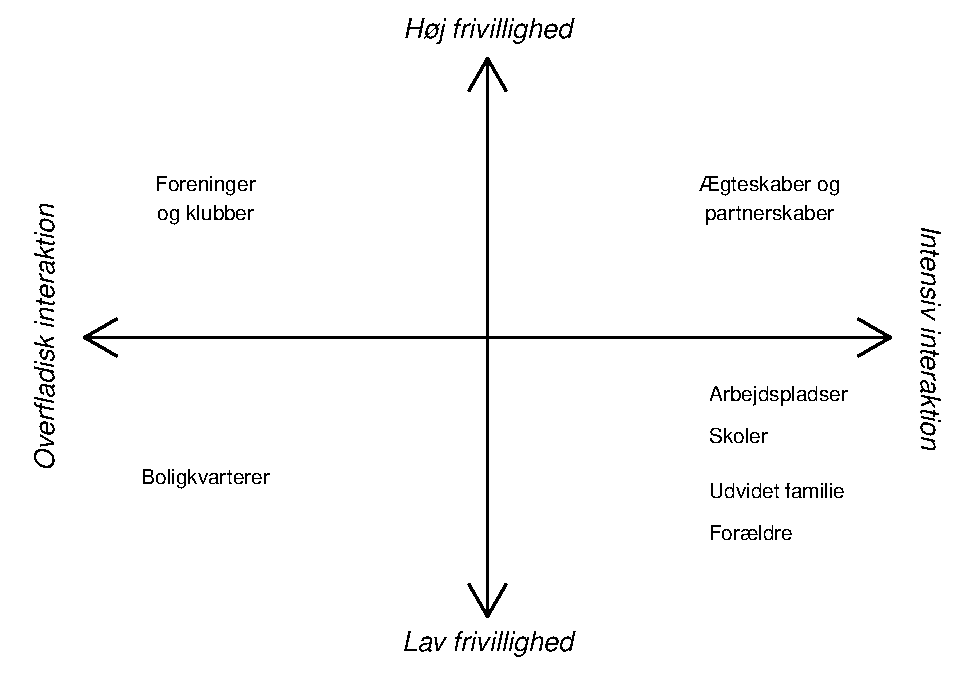
\includegraphics[width=1\linewidth]{en-befolkning-blander-sig_files/figure-latex/fig-1-1-1} \caption{Idealtypiske mødepladser.}\label{fig:fig-1-1}
\end{figure}

Bogen er specielt optaget af de mødepladser, der idealtypisk befinder sig i det nedre højre hjørne af Figur \ref{fig:fig-1-1}. Det er mødepladser med en relativ lav frivillighed, hvilket modvirker menneskers nærmest naturlige søgen efter ligesindede. Det meste ekstreme eksempel på ufrivillighed er, at vi ikke selv vælger vores forældre. Er man barn af et blandet ægteskab kan man dårligt undgå både at møde majoritetsbefolkning og indvandrere. Et mindre ekstremt eksempel er, at man ikke vælger ens bredere familier. Majoritetsbefolkningen kan blive ''udsat'' for børn eller søskende, der vælger indvandrere som partnere. Og omvendt kan indvandrere blive ''udsat'' for børn eller søskende, der vælger majoritetsbefolkning som partnere. Dermed skabes der møder mellem majoritet og indvandrere, der er svære at fravælge. Arbejdspladser og skoler er en anden mødeplads, hvor graden af frivillighed er relativt lav. Man kan ikke frit vælge ens kolleger. Det er en ret, der tilfalder arbejdsgiverne at ansætte og organisere arbejdet. Ligeledes kan skolebørn ikke selv vælge deres klassekammerater. Det afhænger normalt af administrativt fastsatte skoledistrikter. Samtidig er skoler, arbejdspladser og familier mødepladser, hvor interaktionen mellem mennesker ofte er intensiv. Det ekstreme eksempel er igen børn af ''blandede'' partnerskab. Her hænger man år efter år på ens forældre. Men skoler og arbejdspladser kan også være præget af intense og langvarige interaktioner mellem mennesker. Det er ved sådanne intense interaktioner, at potentialet for at nedbryde betydningen af etniske distinktioner er særligt stort. Det er disse tvungne mødepladser med intensiv interaktion, der interesseret os mest.

Dermed også sagt, at andre mødepladser er mindre vigtige for at skabe sociale relationer og tillid mellem etniske grupper. I vores perspektiv er potentialet mindre, hvis mødepladserne er præget af frivillighed og overfladisk interaktion. Et eksempel kunne være et fitnesscenter. Her kan man lade være med at komme, hvis man ikke vil møde minoriteterne eller majoriteten. Samtidigt er interaktionen typisk overfladisk, hvilket gør potentielt for at bygge sociale relationer og nedbryde fordomme mindre. Andre former for fritidsaktiviteter kan skabe mere intensiv interaktion på tværs af etniske grupper, men ikke desto mindre har vi idealtypisk placeret foreninger og klubber i det øvre venstre hjørne af Figur \ref{fig:fig-1-1}. I et integrations- og assimileringsperspektiv er det primære ''problem'' ved foreningsdeltagelsen, at man frit kan vælge hinanden fra eller ligefrem etablere eksklusive foreninger, der kan fordybe betydningen af etniske skillelinjer. Religiøse foreninger er det klassiske eksempel på eksklusive etniske foreninger, men det kan også ske for loger, spejderforeninger og løbeklubber.

I det nedre venstre hjørne har vi idealtypisk placeret boligkvarteret. Her er der tale om en arena, hvor vi har en mere begrænset indflydelse på, hvem vi mødes med. Man kan vælge sin fitnesspartnere, men man kan ikke frit vælge sine naboer. Den mindre frivillighed skulle alt andet lige føre til flere ansigt-til-ansigt-møder mellem indvandrere og majoritetsbefolkningen. I majoritetsbefolkningen er der segmenter, der må søge efter billigere boligområder, hvor der typisk er mange indvandrere, og blandt indvandrere er der segmenter, der har råd til at søge mod majoritetsbefolkningens mere attraktive boligkvarterer. Til gengæld er naboskabet i udgangspunktet en overfladisk interaktion. Man hilser pænt på naboen, men herudover kan interaktionen være meget begrænset. I vores perspektiv er boligkvarteret primært interessant fordi det potentielt påvirker sammensætningen af de tvungne møder med intensiv kontakt i det nedre højre hjørne. Mest oplagt den etniske sammensætning af skolerne, som bliver beskrevet i \hyperref[kap3]{kapitel 3}.

Endeligt har vi det øvre højre hjørne af figur 1, hvor vi idealtypisk har placeret ægteskabet. Her er den fysiske mødeplads typisk en fælles bolig. Det er formentligt den mest intensive interaktion, som man kan forstille sig. Dermed er potentialet til at nedbryde, hvad der måtte være af fordomme stort. I et integrations- og assimileringsperspektiv er det primære ''problem'' ved ægte- og partnerskaber, at frivilligheden er så høj og interaktionen så intens, at man ofte vælger en partner, der ligner sig selv. Derfor er ægte- og partnerskaber typisk med til fastholde, og til tider forstærke, betydningen af etniske skillelinjer. Og dem fra majoriteten og minoriteten, der vælger at indgå i blandede ægte- og partnerskab, er typisk dem, der ikke har mange fordomme at få nedbrudt til at begynde med. Det er én af grundene til, at den amerikanske forskning netop har brugt blandede ægteskaber som en guldstandard for integration/assimilering. En anden mere praktisk grund er, at det har været nemt at skaffe historiske data på ægteskaber. I vores perspektiv er de blandede partner- og ægteskaber primært interessant fordi det skaber ''blandede'' børn, der effektivt nedbryder et samfunds etniske kategorier, og fordi det har effekter på deres bredere familier.

\section{Det menneskelige møde og dets effekt på betydning af etniske distinktioner}\label{det-menneskelige-muxf8de-og-dets-effekt-puxe5-betydning-af-etniske-distinktioner}

Hvad der sker, når mennesker mødes på tværs af etniske skillelinjer er specielt blevet studeret og teoretiseret af socialpsykologien. Socialpsykologiens udgangspunkt er, at negative opfattelser af såkaldte ud-grupper ikke er nogen mærkværdighed. Ifølge socialpsykologien er det (desværre) alment menneskeligt, at grupper af mennesker, definerer sig selv ved at tage afstand fra andre. Det gør sig gældende for små grupper, fx etablerer skoleklasser ofte negative billeder af deres søsterklasser, og for store grupper, fx etablerer folkeslag ofte negative billeder af andre folkeslag. Der er derfor heller ikke noget mærkværdigt i, at majoritetsbefolkninger ofte opbygger negative mentale billeder af indvandrere (og omvendt). Grænsedragningen mellem ''etniske danskere'' og ''indvandrere'' knytter sig til selve fundamentet for dannelsen af nationalstater. Majoritetsbefolkningen skaber internt sammenhold og identitet ved at etablere et negativt billede af ud-grupper. Omvendt kan etniske minoriteter skabe internt sammenhold og identitet ved at etablere et negativt billede af majoritetsbefolkningen.

Det er velkendt fra socialpsykologien, at gruppetilhørsforhold nærmest per automatik skaber positive billeder af ind-gruppen og negative billeder af ud-gruppen. Socialpsykologiske forsøg har vist, at selv simpel gruppedannelse, hvor de involverede personer ved, at de er inddelt helt tilfældigt, skaber intern solidaritet (\citeproc{ref-tajfel1981}{Tajfel, 1981}). Det skaber realistiske forventninger om, at personer i ens ind-gruppe er solidarisk indstillede, mens personer i ens ud-gruppe er fjendtligt indstillede (selv ved helt tilfældig inddeling, fx i blåøjede over for brunøjede).

Den amerikanske socialpsykologi har specielt været optaget af, hvorvidt møder mellem den ''hvide'' majoritet og den ''sorte'' minoritet formindsker eller ligefrem forstærker denne etniske race distinktion. I et klassisk værk fra 1954 beskrev Allport, hvordan kontakt har et potentiale til at nedbryde fordomme på tværs af grupper (\citeproc{ref-allport1954}{Allport, 1954}). Men det er ikke nogen enkel proces. Allport advarede om, at overfladisk kontakt mellem sorte og hvide \emph{ikke} vil nedbryde fordomme. Tværtimod kan fx et overfladisk møde i bybilledet give yderligere næring til fordomme. Den ide havde blandt andet sin baggrund i empiriske studier af, hvorledes hvide nordstats-amerikanere, der uddannede sig i sydstaterne, fik flere og ikke færre fordomme om afroamerikanere. En mulighed er således, at danskere, der bor i boligkvarterer med mange indvandrere, opbygger stærkere negative stereotyper om indvandrere, da der kun er overfladisk kontakt mellem grupperne. Det samme kan formentlig ske med overfladisk kontakt i klubber og foreninger.

Allport mente dog, at nogle typer af kontakt kan reducere fordomme på tværs af grupper. Allport opstillede fire kriterier for, hvornår kontakt kan have sådanne gavnlige effekter. Der skulle være 1) statuslighed mellem grupper, 2) fælles målsætninger, 3) samarbejde på tværs af grupper og 4) opbakning fra autoriteter, lov eller vane. Baggrunden var blandt andet studier, der havde vist, at sorte og hvide soldater, der havde kæmpet sammen i Anden Verdenskrig, havde markant færre fordomme om hinanden (\citeproc{ref-stouffer1949}{Stouffer et al., 1949}). Disse soldater havde haft lige status (rang), de havde haft en fælles målsætning (nedkæmpe fjenden), sorte og hvide havde samarbejdet (i krigshandlingen) og samarbejdet var understøttet af en autoritet (befalingsmænd), der overvågede samarbejdet. Med dette udgangspunkt har en række studier analyseret, hvordan kontakt kan nedbryde fordomme (\citeproc{ref-pettigrew2006}{Pettigrew \& Tropp, 2006}). Det er med baggrund i denne såkaldte kontaktlitteratur, at bogen netop fokuserer på mødepladser mellem lav frivillighed og intensiv interaktion, se ovenstående figur 1.1.

Vi er fuldt bevidste om, at tvungne møder med intensiv interaktion mellem majoritetsbefolkning og indvandrere ikke kun har potentiale til at mindske betydningen af etniske distinktioner. Disse mødepladser kan også skabe konflikter, der kan forøge betydningen af etniske distinktioner. For minoriteten sker det typisk, hvis den oplever, at der ikke er statuslighed i interaktionen. Hvis minoriteten oplever, at de bliver diskrimineret på skolen eller på arbejdspladsen forøges negative ud-gruppeforestillinger. Typisk har efterkommere højere ambitioner om ligebehandling end indvandrere, hvilket afspejler sig i større oplevelse af diskrimination. For majoriteten leder interaktion specielt til konflikt i situationer, hvor etniske minoriteter udgør så stor en andel, at det truer de fordele, som majoriteten har ved at være majoritet (\citeproc{ref-forbes2004}{Forbes, 2004}). Majoritetsfordele kan være alt fra det sprog, der skal tales på arbejdspladsen og i skolens frikvarterer, til, hvad der skal være på menuen til firmafesten. En anden klassisk teori er, at medlemmer af majoriteten specielt føler sig truet, hvis de befinder sig i en udsat position. Det kan være en økonomisk udsat situation, hvor det kan være en frygt, at indvandrere overtager ens job eller (yderligere) forringer arbejdsvilkårene. Men det kan også vær en kulturel udsat situation, hvor det kan være en frygt for, at man kan miste sin status i sin egen ind-gruppe, hvis grænserne til udgruppen eroderes. Ikke desto mindre er bogens perspektiv, at det er på de tvungne mødepladser med intensiv interaktion, at det største \emph{potentiale} for integration ligger.

\section{Betydningen af størrelsesforholdene mellem majoritet og minoritet}\label{betydningen-af-stuxf8rrelsesforholdene-mellem-majoritet-og-minoritet}

Mens socialpsykologien har været optaget af dynamikker i mødet mellem mennesker, så har makrosociologske teoretikere som Blau (\citeproc{ref-blau1984a}{P. M. Blau et al., 1984}; \citeproc{ref-blau1994}{P. M. Blau, 1994}; \citeproc{ref-blau1997}{Peter M. Blau et al., 1997}) været optaget af gruppestørrelsers betydning for muligheden for overhovedet at mødes. For majoriteten kan mulighederne for at møde minoriteten være begrænsede. Tilbage i 1980 udgjorde indvandrere og efterkommere tre procent af befolkningen(ifølge Danmark Statistisk definitioner, hvilket vi skal komme tilbage til i det næste kapitel). Selv hvis indvandrere havde været helt lige fordelt i boligkvarterer, i foreninger, i skoler og på arbejdspladser, ville danskerne (som defineret af Danmark Statistik) kun have tre procent chance for, at det næste ansigt-til-ansigt møde var med en indvandrer. Omvendt ser det selvfølgelig ud for minoriteten. Indvandrere og efterkommere ville have 97 procent chance for, at det næste møde var med en etnisk dansker. Minoriteten eksponeres således markant mere for majoriteten end majoriteten eksponeres for minoriteten -- alt andet lige. Så hvis man antager, at fysiske møder mellem etniske grupper har konsekvenser, så er disse konsekvenser langt mere udbredte blandt minoriteten end majoriteten. Det betyder også, alt andet lige, at integrationens tovejsproces foregår i forskellige hastigheder. Minoriteten ændres hurtigt. Majoriteten ændres langsomt.

De sidste fire årtiers stigende indvandring har ændret disse størrelsesforhold i Danmark. I 2023 udgjorde indvandrere og efterkommere 15 procent af befolkningen ifølge definitioner fra Danmark Statistik. Under antagelse om lige fordeling på mødepladser, er danskernes sandsynlighed for næste gang at møde en indvandrer eller efterkommer således steget fra tre til 15 procent. Omvendt er minoritetens sandsynlighed for næste gang at møde en dansker reduceret fra 97 til 85 procent. Følger man ovenstående logik vil det betyde, at majoriteten ændres lidt hurtigere og minoriteten lidt langsommere end det var tilfældet tidligere.

Effekterne af disse størrelsesforhold på antallet af møder mellem minoritet og majoritet begrænses selvfølgelig af de strukturelle forhold, der typisk koncentrerer indvandrere i byområder, jf. ovenstående. I Figur \ref{fig:fig-1-2} vises andelen af indbyggere, der ikke har to forældre med dansk herkomst. Med vores strammere kriterier for at være dansk-dansk (se næste kapitel for definitioner) illustrerer kortet med alt tydelighed, at der også i Danmark er en betydelig koncentration af minoriteter i byområderne. I kapitel 5 vil det nærmere blive beskrevet, hvordan danskere i nogle kommuner har ret begrænsede muligheder for at danne sociale relationer med indvandrere; specielt hvis man også medtænker et alderskriterium ift. hvem man forventeligt danner sociale relationer med.

\begin{figure}
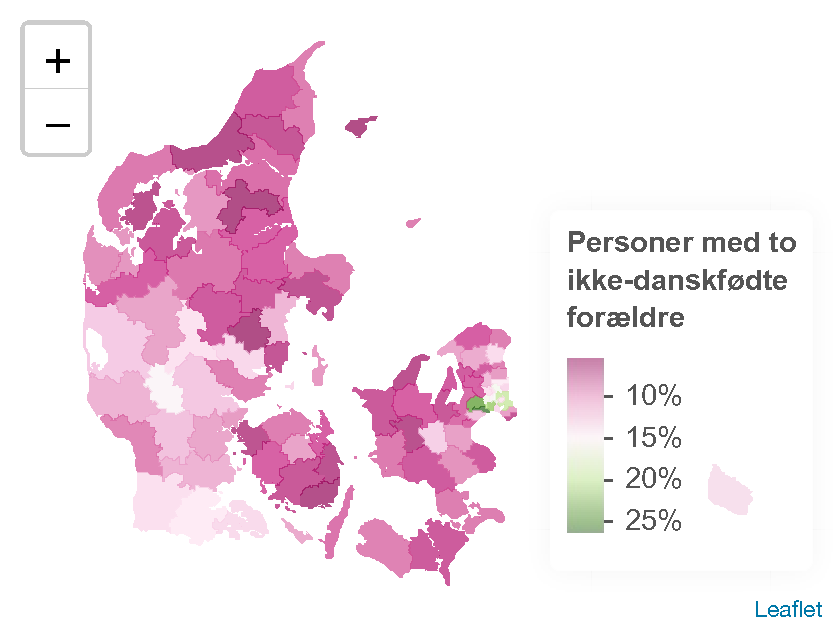
\includegraphics[width=1\linewidth]{en-befolkning-blander-sig_files/figure-latex/fig-1-22-1} \caption{Andelen af indbyggere, hvor begge forældre ikke har dansk herkomst. 2024. <br> Note: *Baseret på FOLK1B 2024K2*.}\label{fig:fig-1-22}
\end{figure}

Hvorvidt indvandreres større mulighed for at møde andre indvandrere reelt begrænser antallet af møder med majoritetsbefolkningen er omstridt. Den dominerende hypotese i den amerikanske integrationslitteratur er, at en større gruppe fra ens egen nationalitet, fx italienere eller mexicanere, kan virke som en trædesten, der gør det nemmere for en nytilkommen indvandrer at få kontakt med majoriteten, og de heraf følgende ofte forberede livsmuligheder. Denne optimistiske udlægning baseret på historiske amerikanske erfaringer er dog problematiseret af nyere teoriretninger. Såkaldt segmenteret assimileringsteori (\citeproc{ref-portes1993}{Portes \& Zhou, 1993}) fremhæver, at den effekt afhænger af ''kvaliteten'' af indvandrere med ens egen nationalitet, der er i landet. Hvis ens nationalitet klarer sig dårligt i uddannelsessystemet og på arbejdsmarkedet kan det virke hæmmende og ikke befordrende for en nytilkomnes livsmuligheder. Teorien fremhæver også, at post-moderne økonomier skaber en segmentering af arbejdsmarkedet, hvilket gør det vanskeligt tale om en majoritetsbefolkning med rimeligt ensartede livsvilkår, som indvandrere langsomt integreres i. Den alternative hypotese er, at indvandrere lige så vel kan integreres ind i et underklasse- eller overklassesegment i destinationslandet.

\section{Den danske versus den amerikanske kontekst}\label{den-danske-versus-den-amerikanske-kontekst}

Bogen bygger på en antagelse om, at de grundlæggende mekanismer omkring indvandrere og majoritetsbefolkning er de samme i Danmark som i USA. Mekanismerne er knyttet til grundlæggende egenskaber ved den menneskelige natur, ved en verden opdelt i nationalstater og ved markedsøkonomier. Ikke desto mindre er der åbenlyse forskelle med den danske kontekst og den amerikanske både historiske og nuværende kontekst. Én markant forskel er, at Danmark har en større andel humanitære indvandrere end det er tilfældet i USA. Disse flygtninge og familiesammenførte har ofte sværere ved at klare sig på arbejdsmarked end indvandrere, hvor den primære motivation til at skifte land netop har været ønsket om arbejde. Til gengæld har humanitære indvandrere typisk ikke noget ønske om at vende tilbage til et oprindelsesland. Der er således ikke anden udvej end at forsøge at klare sig i destinationslandet. Dermed har de humanitære indvandrere større incitament til at lade sig integrere end arbejdsimmigranter.

Én anden markant forskel er, at Danmark har et mere reguleret arbejdsmarked end det er tilfældet i USA. Det skaber bedre løn-- og arbejdsvilkår, også for indvandrere, hvilket alt andet lige må antages at lette integrationen. Men samtidigt kan reguleringerne gøre det vanskeligere for indvandrere at komme ind på arbejdsmarkedet, fx ved ikke at kunne acceptere lavere løn- og arbejdsvilkår end majoritetsbefolkningen. Risikoen ved et reguleret arbejdsmarked er således, at flere indvandrere slet ikke kommer ind på arbejdsmarkedet end det er tilfældet på det mere uregulerede amerikansk arbejdsmarked.

Én tredje forskel er, at Danmark har en mere udbygget velfærdsstat, der leverer sygesikring, børnepasning og skoleundervisning af relativt høj kvalitet for alle; inklusive indvandrere uden statsborgerskab. Det letter presset for at klare sig på arbejdsmarkedet, men forøger samtidigt majoritetsbefolkningens bekymring for at indvandrere bliver en økonomisk byrde.

Endeligt er der markant mere politisk regulering i Danmark end i USA. I årtier har Danmark således ført en politik, der aktivt har forsøgt at understøtte møder mellem danskere og indvandrere/efterkommere, og reducere interne møder mellem sidstnævnte. Mest omdiskuteret er de offentlige politikker om boligplacering af humanitære indvandrere, der siden 1999 er blevet spredt i landets kommuner. I den første treårige periode mister flygtninge retten til kontanthjælp, hvis de fraflytter den tildelte kommune. Siden 1994 har skriftende regeringer også gennemført en række ''ghetto-planer'', der har til hensigt at forhindre koncentration af indvandrere og efterkommere i specifikke boligkvarterer. I skrivende stund implementeres en bred politisk aftale kaldet ''Blandede boligområder -- næste skridt i kampen mod parallelsamfund. Endeligt har de danske kommuner i årtier aktivt forsøgt at sammensætte grundskoler, så majoritetens og indvandrernes børn møder hinanden. Specielt har man været optaget af at forhindre grundskoler, hvor indvandrere udgør en numerisk majoritet. Dertil kommer en myriade af andre integrationspolitikker, der primært drives af landets jobcentre. Her har man i mere end 30 år eksperimenteret med politikker, der i særdeleshed har fokuseret på at forøge beskæftigelsen blandt indvandrere og efterkommere. Man kan sige, at man i Danmark vi offentlig politik aktivt har forsøgt at påvirke møderne mellem majoritets- og minoritetsbefolkningen, mens man i USA mere passivt har accepteret, at integration tager tid. Aktiv amerikansk ''blandingspolitik'' har primært fokuseret på at afskaffe de diskriminerede politikker over for sorte; suppleret med aktive politiker som ''affirmative action'', der forsøger at skabe social mobilitet for denne specifikke gruppe.

Aktiv offentlig politik kan formentlig forøge møderne mellem majoriteter og indvandrere, men vores fornemmelse er, at effekten er mindre end ofte antaget i den offentlige debat. Bogens antagelser er, at møderne mellem danskerne og indvandrere primært er styret af mekanismer, der er begrænset politisk kontrol over. Antagelsen er, at det er forhold som forelskelse, priser på boligmarkedet, jobmuligheder og menneskers ønske om at være vellidt i en gruppe, der er de primære drivkræfter i nedbrydningen etniske distinktioner.

\section{Bogens plan}\label{bogens-plan}

I \hyperref[kap2]{kapitel 2} beskriver vi, hvordan partnerskaber i Danmark typisk etableres indenfor samme etniske gruppe. Men antallet af tværetniske partnerskaber er dog stigende og deraf følger en gruppe af børn med ''blandet'' etnisk baggrund. \hyperref[kap3]{Kapitel 3} beskriver, hvordan de kategorier, der typisk anvendes i Danmark, overser denne gruppe af børn og unge. Derfor etableres en alternativ kategorisering, der også vil blive brugt i bogens efterfølgende kapitler.

\hyperref[kap4]{Kapitel 4} beskriver den etniske sammensætning af danske grundskoler. Kapitlet viser, at den etniske opdeling generelt er moderat og faldende over tid i Danmark. Etnisk opdeling er et mere snævert storbysfænomen, der både skyldes bosætningsmønstre og muligheden for alternative skoler indenfor en kort afstand. \hyperref[kap5]{Kapitel 5} beskriver vi den etniske sammensætning af danske arbejdspladser. Kapitlet viser, at de danske arbejdspladser bliver mere etnisk opdelt. Men samtidigt viser kapitlet, at trods disse velkendte segmenteringstendenser på arbejdsmarkedet, så arbejdere flere og flere med dansk oprindelse sammen med indvandrere og efterkommere.

Efter disse kapitler, der primært beskriver forudsætningerne for at etablere sociale relationer mellem danskere, indvandrere og efterkommere, beskriver \hyperref[kap6]{kapitel 6} omfanget af venskabsrelationer på tværs etniske skel. Kapitlet viser, at langt de fleste indvandrere og efterkommere har danskere i deres omgangskreds, og langt de fleste danskere har indvandrere og efterkommere i deres omgangskreds. Undtagelsen er ældre danskere bosat i landkommuner, hvor muligheden for at mødes med indvandrere og efterkommere er begrænset.

Endeligt diskuterer vi det afsluttende \hyperref[kap7]{kapitel}, hvordan bogens fokus på tværetniske sociale relationer adskiller sig fra andre forståelser af integration. Bogen er en formidlingsbog, der sammenfatter resultater fra en større dansk forskningsprojekt, som allerede nævnt forordet. Ikke desto mindre inkluderer bogen et teknisk appendiks, der omhandler de statistiske metoder og mål, der anvendes til at beskrive skillelinjer på tværs af etniske skel.

\chapter{Tværetniske partnerskaber}\label{kap2}

\emph{\href{https://vbn.aau.dk/da/persons/hpq}{Hans-Peter Y. Qvist}}


\includegraphics[width=1\linewidth]{images/dalle-wedding}

Et fast forhold eller ægteskab er den dybeste og mest forpligtende sociale forbindelse, man kan have med en anden person. Derfor er det at vælge en fast partner en af de vigtigste beslutninger, vi træffer. Vælger vi den rette partner, kan det berige vores liv markant. Omvendt kan et forkert valg føre til dybe materielle, følelsesmæssige og sociale tab, især hvis det ender i skilsmisse. De betydelige konsekvenser af at vælge en partner fører sandsynligvis til, at mange mennesker foretrækker en følelse af sikkerhed i deres valg. Modsat den populære forestilling om, at modsætninger tiltrækker hinanden, viser omfattende samfundsvidenskabelig forskning nemlig, at vi mennesker typisk vælger en partner, der ligner os selv på en lang række områder. Det gælder socioøkonomiske faktorer som uddannelse, job og indkomst såvel som kulturelle faktorer som etnicitet, religion, værdier (\citeproc{ref-kalmijn1998}{Kalmijn, 1998}).

I lyset af tendensen til at folk typisk vælger partnere, der ligner dem selv, er det ikke overraskende, at indvandrere og deres efterkommere i Danmark og andre lande ofte foretrækker partnere fra deres egne oprindelseslande. Der er imidlertid store forskelle på hvor udbredt denne tendens er imellem forskellige indvandrergrupper. I nogle indvandrergrupper er det nok mere hyppigt, at man danner par indenfor gruppen end tilfældigheder ville tilsige, men der er omvendt også mange der danner par udenfor gruppen. I andre indvandrergrupper er tendensen til at vælge partnere inden for gruppen meget stærkere, og tværetniske forhold er derfor sjældnere.

I dette kapitel giver jeg i det først afsnit en kort introduktion til den sociologiske forskning på området og beskriver herefter udbredelsen af tværetniske ægteskaber i Danmark. I det tredje afsnit referes hovedkonklusionerne fra studiet af Qvist \& Qvist (\citeproc{ref-qvistqvist2023}{2023}), der giver en række forklaringer på mønstrene for tværetniske partnerskaber i Danmark. I det sidste afsnit diskuterer jeg det svære spørgsmål om, hvorvidt de danske partnerskabsmønstre viser, at glasset er halvt fyldt eller halvt tomt.

\section{Sociologien om de tværetniske partnerskaber}\label{sociologien-om-de-tvuxe6retniske-partnerskaber}

I sociologien er der en lang tradition for at undersøge årsager og konsekvenser af forskelle i minoritetsgrupper tendens til, at danne par inden- eller udenfor egen gruppe. Det skyldes en forventning om, at udbredelsen af tværetniske ægteskaber, især mellem repræsentanter for indvandrergrupper og majoritetsbefolkningen, kan give en klar indikation på, hvor socialt integrerede indvandrergrupper er i destinationslandet. En af de mest markante repræsentanter for dette perspektiv, den amerikanske sociolog Milton M. Gordon (\citeproc{ref-gordon1964}{1964}), argumenterede således for, at udbredelsen af tværetniske parfold er den ultimative indikation på, at barrierer mellem etniske grupper nedbrydes og at den sociale sammenhængskraft styrkes.

Ægteskabets rolle i at forene mennesker er et velkendt fænomen gennem historien. Traditionelt har ægteskaber ofte været brugt til at skabe alliancer mellem familier eller endda hele kongeriger. I den tidlige middelalder var det fx almindeligt, at den romerske elite i Vesteuropa indgik ægteskaber med ledere af indvandrende stammer. Dette førte til en kulturel fusion mellem den romerske kultur og stammernes traditioner (OBS Wickham, 2009 OBS). Samtidig kunne det være en måde at skabe mere fred og mindre konflikt.

I vore dage kan tværetniske ægteskaber mellem helt almindelige mennesker stadig have stor betydning. Det er der flere forskellige grunde til. For det første indikerer dannelsen af tværetniske parforhold, at fordomme og sociale grænsedragninger mellem etniske grupper ikke er stærke nok til at forhindre dannelsen af intime og tillidsfulde relationer mellem to personer fra forskellige etniske grupper. Dette kan være afgørende for, at barriere nedbrydes yderligere mellem grupperne. For det andet forener et blandet par typisk ikke kun to individer, men også deres familie og venner. Personer der indgår i blandede par kan således agere brobyggere mellem sociale netværk eller grupper, som ellers ikke ville have megen kontakt med hinanden. For det tredje har børn fra blandede parforhold en unik position, når det kommer til at udviske kulturelle forskelle, hvilket vil blive udforsket yderligere i \hyperref[kap3]{kapitel 3}.

Det er afgørende at forstå, at den sociologiske forskning, som undersøger konsekvenserne af etnisk blandende parforhold---eller mangel herpå---hovedsageligt betragter effekterne på samfundsplan. Disse teorier fremhæver, at selvom det for den enkelte indvandrer kan virke naturligt og forenkle livet at vælge en partner med samme etniske baggrund, kan denne tendens medføre udfordringer for samfundet og for etniske grupper som helhed, særligt når mange indvandrere fra specifikke grupper systematisk foretrækker partnere fra deres eget oprindelsesland, idet det medvirker til at lukke grupperne om sig selv og bidrager til etnisk segregering.

\section{Tværetniske partnerskaber i Danmark}\label{tvuxe6retniske-partnerskaber-i-danmark}

I det følgende skal vi derfor se nærmere på omfanget af tværetniske partnerskaber i Danmark. I Figur \ref{fig:fig-2-1} vises andelen af samtlige partnerskaber blandt bosatte i Danmark, hvor partnerne har samme oprindelsesland og eller andet oprindelsesland.

\begin{figure}
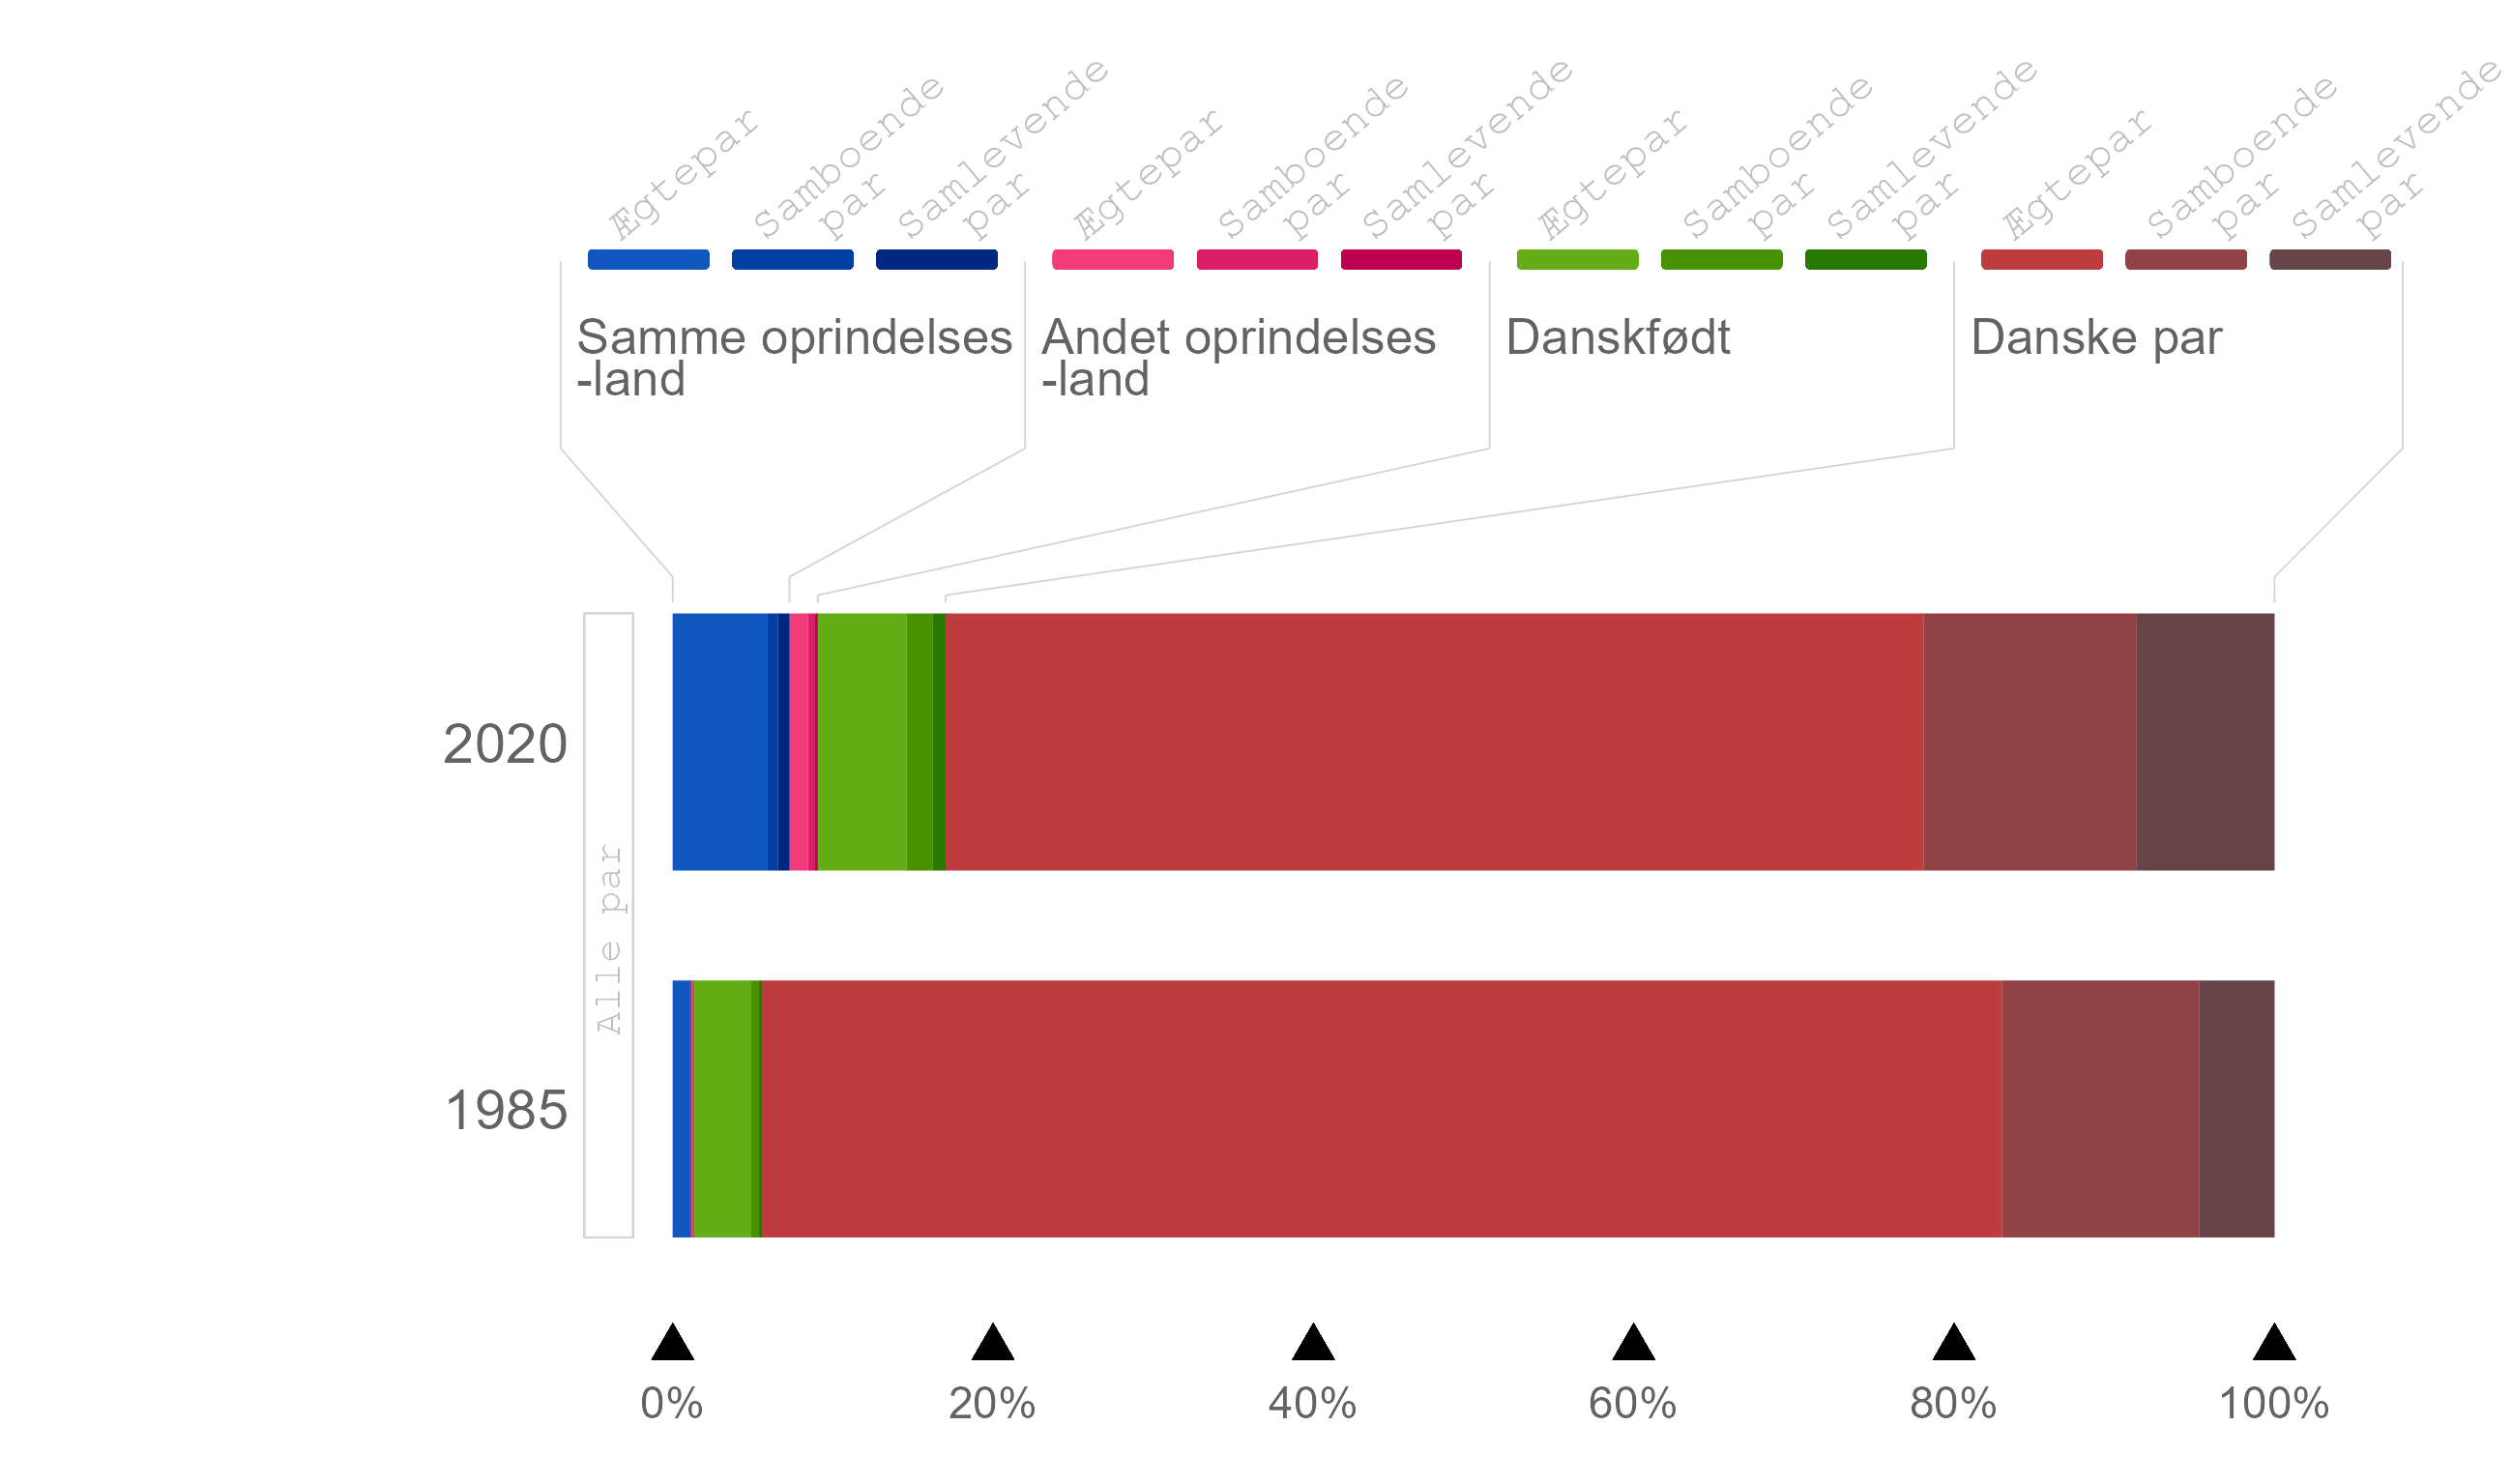
\includegraphics[width=1\linewidth]{images/figur_intergruppepartnerskaber_alle} \caption{ Partnerskaber med samme og forskelligt oprindelsesland. Opgjort i 1985 og 2020.}\label{fig:fig-2-1}
\end{figure}

Det velkendte mønster er, at hovedparten af partnerskaber både i 1985 og 2020 er etableret blandt personer med samme oprindelsesland. Ikke desto mindre viser opgørelsen, at andelen af tværetniske partnerskaber er stigende. Fra femXXX procent i 1985 til 10XXX procent i 2020.

I Figur \ref{fig:fig-2-2} viser den øverste bjælke partnerskabsmønstrene i 2020 blandt alle indvandrere, mens de underliggende bjælker viser mønstrene for ti største indvandrergrupper (der er i partnerskaber med bosatte i Danmark i 2020).

\begin{figure}
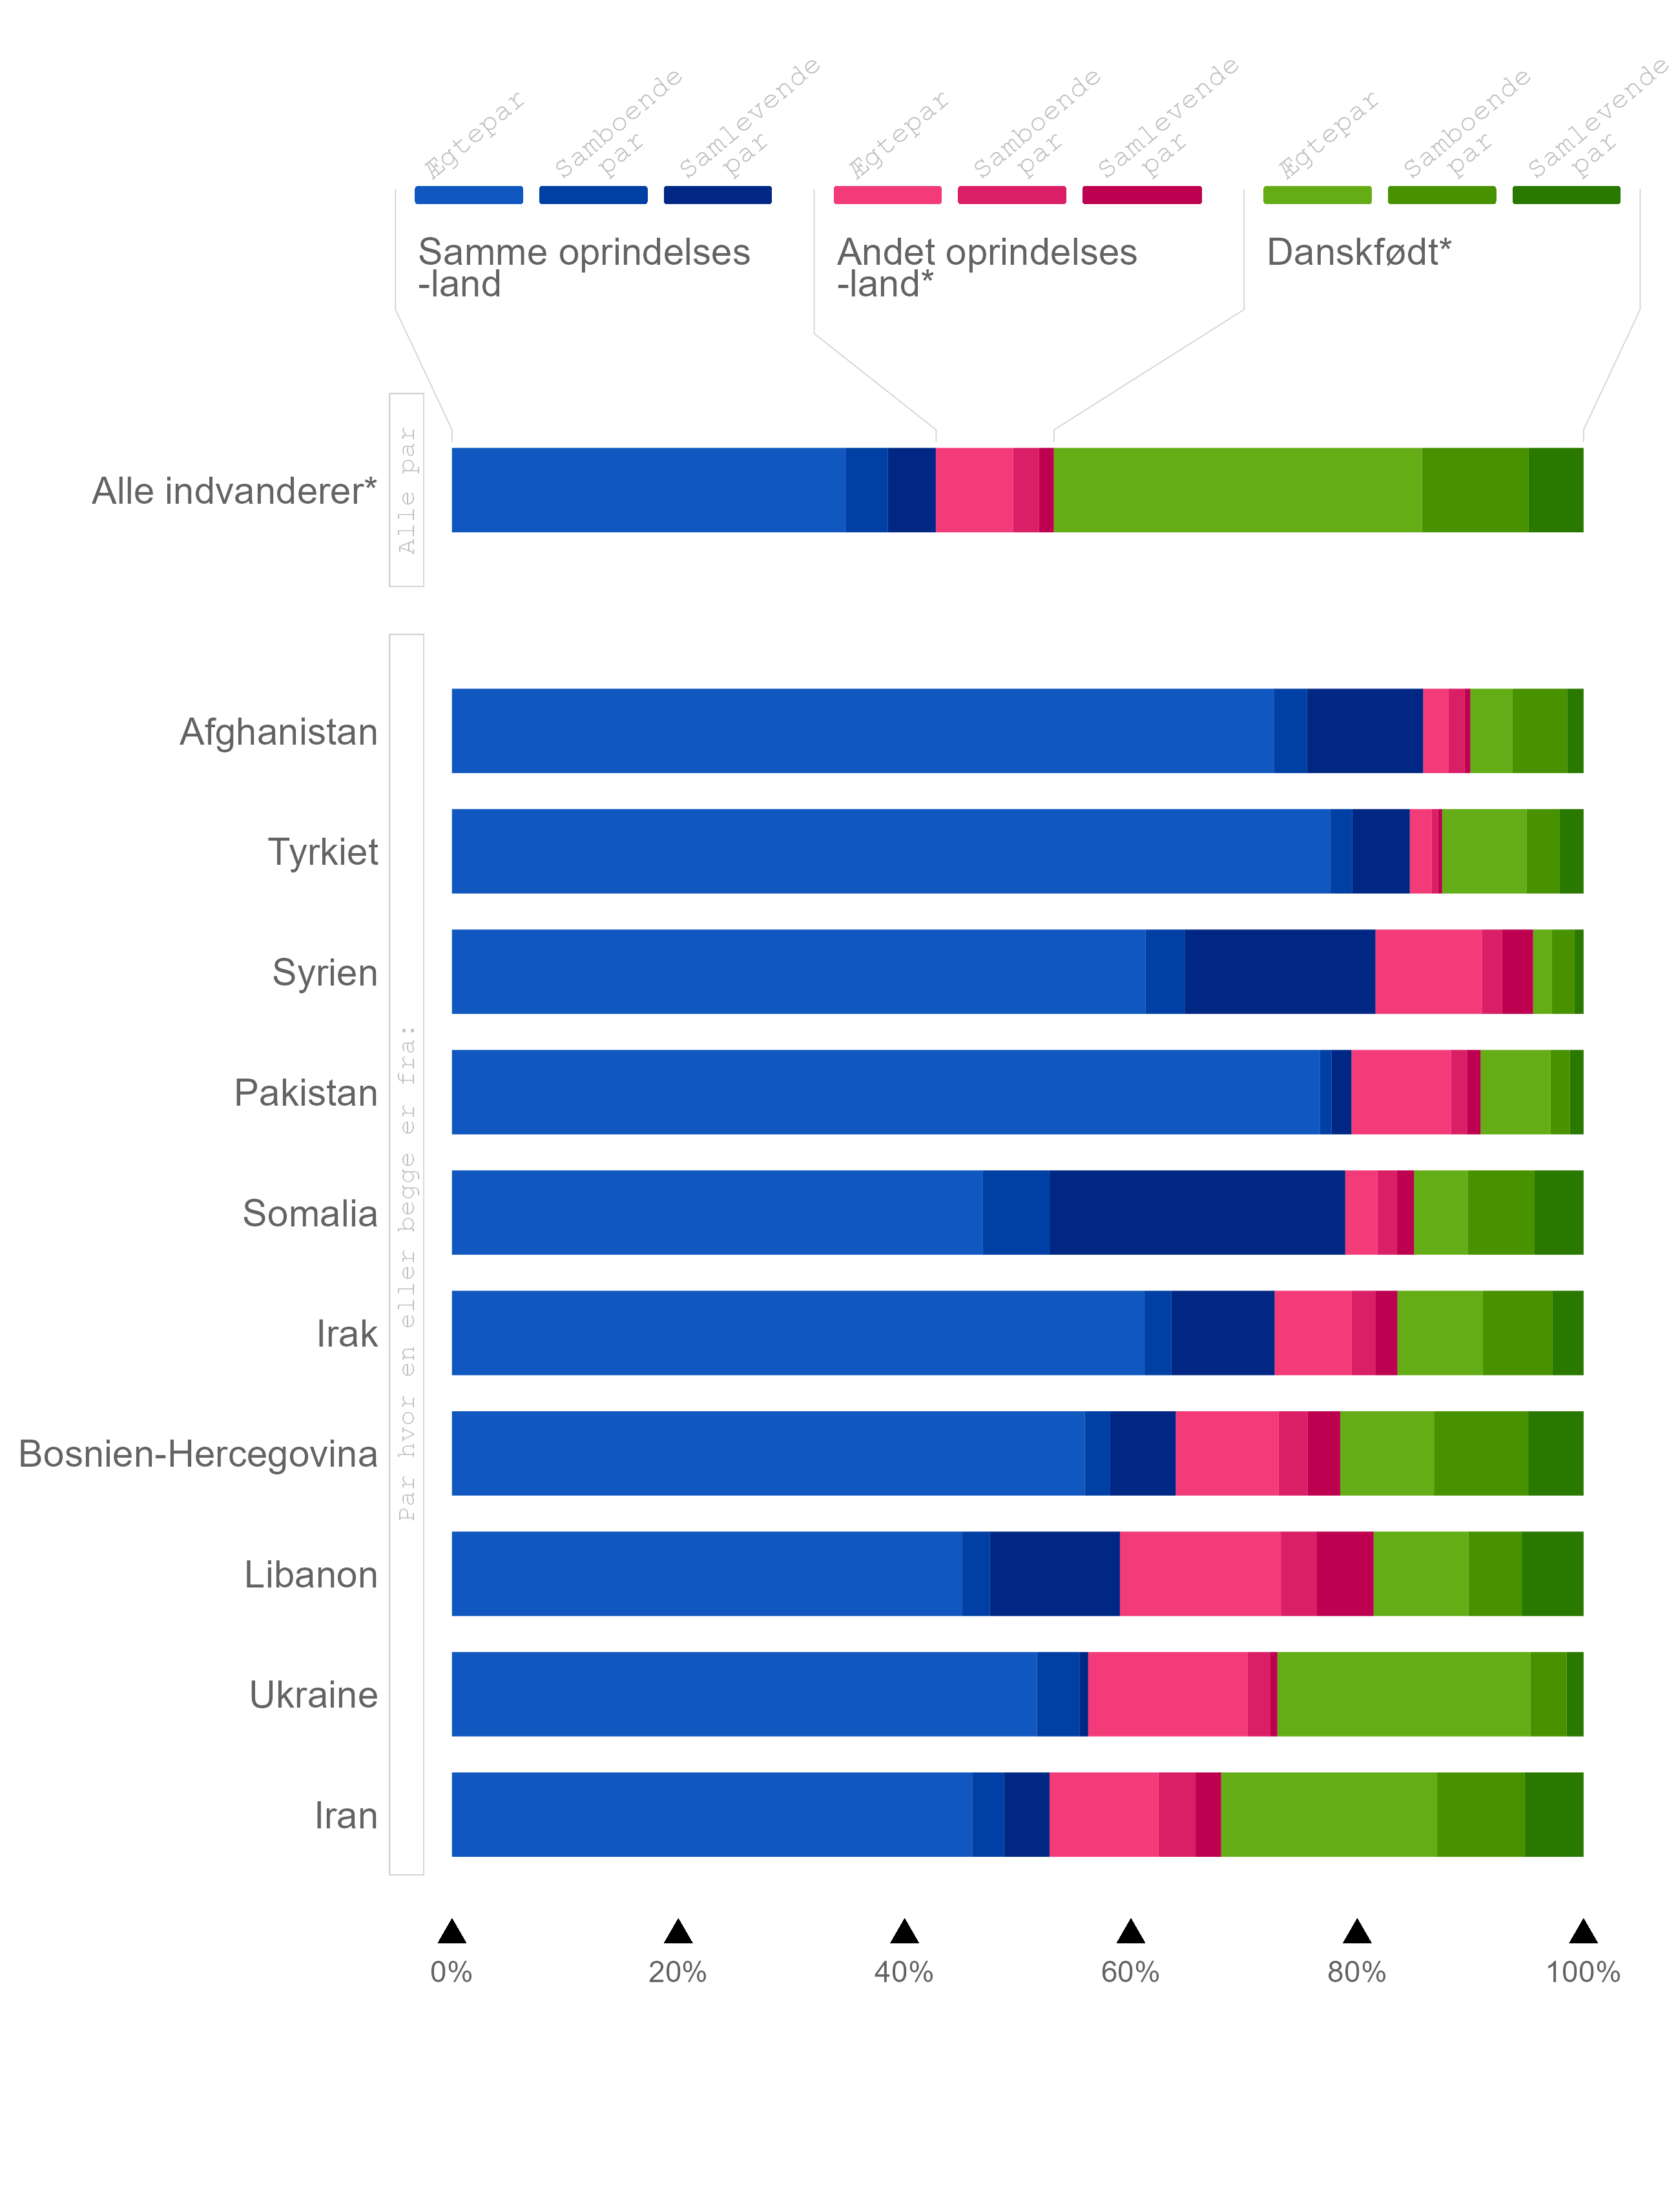
\includegraphics[width=1\linewidth]{images/figur_intergruppepartnerskaber_2020} \caption{Tværetniske partnerskab i 2020.}\label{fig:fig-2-2}
\end{figure}

I 2020 var XXX procent af indvandrere (i partnerskab) i parforhold mellem en person fra samme oprindelsesland, som dem selv. XX procent havde en partner med dansk oprindelse. Endeligt havde et mindretal på XXX procent en partner fra et andet oprindelsesland, end deres eget (og Danmark). Næste del af figuren viser, at der i nogle indvandrergrupper er en stærkere tendens til at danne par med personer fra eget oprindelsesland. Dette pardannelsesmønster er mest udbredt blandt indvandrere med Tyrkisk, Pakistansk og Somalisk baggrund. Omvendt er partnerskab med danskere mest udbredt blandt indvandrere fra Ukraine, Iran og Bosnien-Herzegovina.

\section{Forklaringer på mønstre i tværetniske partnerskaber}\label{forklaringer-puxe5-muxf8nstre-i-tvuxe6retniske-partnerskaber}

Der er mange årsager til, at visse grupper overvejende danner par indenfor deres egen gruppe. Forskningen peger typisk på tre hovedforklaringer: personlige præferencer, strukturelle vilkår, og påvirkning fra eksterne parter (\citeproc{ref-kalmijn1998}{Kalmijn, 1998}). Personlige præferencer dækker over de normer og værdier, der er fremherskende i forskellige grupper, og som kan skabe forhindringer for etableringen af parforhold på tværs af etniske eller kulturelle skel. Strukturelle vilkår handler om de praktiske muligheder for at møde og danne par med nogen fra samme gruppe, hvilket blandt andet kan være betinget af størrelsen på en indvandrergruppe i Danmark og lokalområdet. Endelig omfatter påvirkning fra eksterne parter fx religiøse ledere eller institutioner, der råder imod eller direkte forbyder relationer udenfor egen tro.

Dansk forskning i blandede parforhold er begrænset, men Qvist og Qvist (\citeproc{ref-qvistqvist2023}{2023}) har gennemført et omfattende studie, der har fulgt over 70.000 personer med indvandrerbaggrund fra de fyldte 18 år, indtil de enten flyttede sammen med en partner eller blev gift. De personer som studiet fulgte var enten kommet til Danmark før de fyldte 15 år eller var født i Danmark. Derudover havde de rødder i 120 forskellige lande, hvilket gav en unik mulighed for at kaste lys over betydningen af individuelle præferencer på den ene side og de strukturelle betingelser på den anden, i forbindelse med etablering af parforhold.

Studiet peger generelt på, at jo større kulturelle forskelle der er mellem indvandrergruppen og majoritetsbefolkningen i Danmark, desto mindre er sandsynligheden for, at medlemmer af indvandrergruppen danner par med en person med dansk oprindelse. Den mest betydningsfulde kulturelle faktor er religion. Studiet viser, at personer med indvandrerbaggrund fra ikke-kristne lande har mindre sandsynlighed for at danne par med personer med dansk oprindelse og større sandsynlighed for at danne par med baggrund i eget oprindelsesland end personer med baggrund i andre lande. Samtidig viser studiet, at der er betydelige kønsforskelle.

Når der statistisk justeres for en lang række socioøkonomiske og demografiske faktorer, viser studiet at chancen (oddset) for at mænd med indvandrerbaggrund i overvejende muslimske lande danner par med kvinder med dansk oprindelse er ca. halvt så stort som for mænd med baggrund i protestantiske lande. Det samme gælder for mænd med baggrund i Hinduistiske og Buddhistiske lande. For kvinder med baggrund i muslimske lande er chancen for at danne par med en mand med dansk oprindelse ca. en tredjedel så stort som for kvinder med baggrund i protestantiske lande. For kvinder med baggrund i Hinduistiske og Buddhistiske lande er der imidlertid ikke signifikant forskel på deres chance for at danne par med en mand med dansk oprindelse.

Udover betydningen af religion kaster studiet også lys over den rolle strukturelle betingelser spiller. Her viser studiet, at personer med indvandrerbaggrund som tilhører store indvandrergrupper i Danmark, alt andet lige, har større chance for at danne par med en person med baggrund i eget oprindelsesland.

Endeligt viser studiet at personer med indvandrerbaggrund som er født i Danmark er mere tilbøjelig til at danne blandede par end dem som kom hertil som børn. Dette indikerer, at der sker en udvikling over tid og generationer, hvor personer med indvandrerbaggrund bliver mere tilbøjelige til at danne par med personer med dansk oprindelse, hvilket gælder alle grupper inklusiv kvinder med baggrund i overvejende muslimske lande.

\section{Er glasset halvt fuldt eller halvt tomt?}\label{er-glasset-halvt-fuldt-eller-halvt-tomt}

I den danske offentlige debat fremhæves der ofte forskellige aspekter af virkeligheden alt efter hvilket politisk udgangspunkt man har. Politikere og debattører på højrefløjen fremhæver ofte, at det blandt nogle indvandrergrupper er ganske stor andel som danner par med personer fra deres egne hjemlande. Omvendt fremhæver politikere og debattører fra venstrefløjen typisk, at der sker en udvikling på området, som går i retning af flere tværetniske ægteskaber ikke mindst blandt efterkommere af indvandrere.

Lidt populært kan man sige at der er tale om en diskussion af, hvorvidt glasset er halvt tomt eller halvt fuldt. På den ene side er det rigtigt, at der blandt nogle indvandrergrupper er en stærk tendens til at danne par indenfor egen gruppe både i første og anden generation. På den anden side er det også rigtigt, at der indenfor grupperne sker en udvikling over tid og generationer, hvor tværetniske pardannelse bliver hyppigere. Optimisten vil glæde sig over denne udvikling, mens pessimisten vil sige, at den går for langsomt. Under alle omstændigheder betyder det stigende antal tværetniske partnerskaber, at flere og flere børn har en ''blandet'' etnisk baggrund, hvilket vi skal se nærmere på i det næste \hyperref[kap3]{kapitel}.

\chapter{De blandede børn}\label{kap3}

\emph{\href{https://vbn.aau.dk/da/persons/jeppefl}{Jeppe Fjeldgaard Larsen}} og \emph{\href{https://vbn.aau.dk/en/persons/albrekt}{Christian Albrekt Larsen}}


\includegraphics[width=1\linewidth]{images/dalle-wedding}

I dette kapitel beskriver vi fremkomsten og omfanget af en ny kategori af børn med blandet etisk baggrund. Disse børn medvirker naturligt til at udviske etniske grænsedragninger, da de ikke kan placeres i gamle ''os'' og ''dem'' kategorier.\footnote{Dele af teksten er direkte baseret på Larsen, J. F., \& Larsen, C. A. (2022). Herkomst blandt 0 -- 16-årige bosat i Danmark: Stigende etnisk diversitet og koncentration fra 1985 til 2019. \emph{Metode \& Forskningsdesign}, (4), 47-68. Vi takker tidsskriftet for lov til at genoptrykke dele af teksten.} Opgaven besværliggøres af, at kategorien ikke findes hos Danmark Statistik. Kapitlet starter med en introduktion til de eksisterende kategorier, som Danmark Statistik bruger til at dele befolkningen op i danskere, indvandrere og efterkommere. En opdeling som vi lidt lemfældigt har brugt i de forudgående kapitler. Dernæst udvikler vi en ny kategorisering, der kan indfange fremkomsten af børn med blandet etnisk herkomst. Disse kategorier bruges i det tredje afsnit til at beskrive udviklingen i antallet af disse børn. Vi beskriver de 0--16-årige i perioden fra 1985 til 2019. I det tredje afsnit beskriver vi, hvordan partnerskabsmønstrene ser ud hos disse ''blandede'' børn. I det afsluttende afsnit diskuterer vi kort resultater i relation til konklusionerne fra \hyperref[kap2]{kapital 2}.

\section{Hidtidige statistiske begreber}\label{hidtidige-statistiske-begreber}

Det danske CPR-register og de eksisterende klassifikationer foretaget af DST giver et godt udgangspunkt for at give en beskrivelse af integrationsprocesser. Andre lande, for eksempel USA og Storbritannien, har haft en spørgeskematradition (\citeproc{ref-mendez2013}{Méndez \& Font, 2013}). I forhold til etnicitet har spørgeskematraditionen den fordel, at der kan laves kategorier, hvor befolkningen selv kan angive deres tilhørsforhold, herunder tilhørsforhold på tværs af etniske grupper. Den registerbaseret tradition er mindre sensitiv over for egne klassifikationer. Derfor kan det være vanskeligt at ''opdage'' de blandede børn og deres udviskning af etniske distinktioner.

DST udnytter som udgangspunkt både forældrenes fødested og statsborgerskab samt individets eget fødested til at afgrænse ''dansk herkomst'', ''indvandrere'' og ''efterkommer''. En person med ''dansk herkomst'' er en person - uanset fødested - der har mindst én forælder, der både er dansk statsborger og født i Danmark. Kombination af forældres statsborgerskab og fødested i Danmark bidrager til at afgrænse en relativt etnisk homogen gruppe af ''danskere''. Den manglende betydning af eget fødested bidrager til at inkludere dem, der er født af danske forældre under, ofte midlertidige, ophold i udlandet. Disse børn født i udlandet ligner på sprog, kultur og hudfarve ofte børn af ''danskere'' født i Danmark. Ligeledes har de typisk dansk statsborgerskab.

En ''indvandrer'' er født i udlandet. Ingen af forældrene må være både danske statsborgere og født i Danmark.\footnote{Hvis der ikke findes oplysninger om nogen af forældrene, og personen er født i udlandet, opfattes personen også som indvandrer.} En efterkommer er født i Danmark. Ingen af forældrene må være både danske statsborgere og født i Danmark.\footnote{Hvis der ikke findes oplysninger om nogen af forældrene, og personen er udenlandsk statsborger, opfattes personen også som efterkommer. Når én eller begge forældre, der er født i Danmark, opnår dansk statsborgerskab, vil deres børn ikke længere blive klassificeret som efterkommere. Fastholder danskfødte forældre imidlertid begge et udenlandsk statsborgerskab, vil deres børn forblive klassificeret som efterkommere.} For ''indvandrere'' og ''efterkommere'' opgør DST også oprindelseslandet. Når begge forældre kendes, defineres oprindelsesland ud fra moderens fødeland, henholdsvis statsborgerskabsland. Når kun én forælder kendes, defineres oprindelseslandet ud fra dennes fødeland.\footnote{Hvis dette er Danmark, bruges statsborgerskabslandet. Når ingen af forældrene kendes, er oprindelseslandet defineret ud fra personens egne oplysninger. Er personen indvandrer, antages det, at oprindelseslandet er lig med fødelandet. Er personen efterkommer, antages det, at oprindelseslandet er lig med statsborgerskabslandet.}

Skelnen mellem vestlige og ikke-vestlige indvandrere og efterkommere har været mere kontroversiel. De vestlige lande defineres som alle fra de 27 EU-lande (og det tidligere medlem Storbritannien), Andorra, Island, Liechtenstein, Monaco, Norge, San Marino, Schweiz, Vatikanstaten, Canada, USA, Australien og New Zealand opgøres som vestlige. Alle øvrige lande opgøres som ''ikke-vestlige''. Kategorien ''vestlig'' afgrænser en gruppe, hvor befolkninger målt på velstandsniveau (relativt velstående), religion (relativt kristne) og hudfarve (relativt hvide) nogenlunde ligner hinanden. Det, der karakteriserer de ''ikke-vestlige'', er derfor, at de ikke har denne kombination. Den sociologiske mening bag ''ikke-vestlige'' er således, at gruppen på forskellige parametre er mere afvigende fra majoritetsbefolkningen end ''vestlige'' indvandrere. De ''ikke-vestlige'' vil typisk også være en synlig minoritet på grund af ikke-hvid hudfarve og store dele har muslimsk baggrund.\footnote{En arbejdsgruppe hos DST har set på denne vestlige og ikke-vestlige opdeling og anbefaler at opretholde distinktionen på grund af tydelig sammenhæng mellem denne klassificering og mål for (manglende) integration (Danmarks Statistik, 2019). Argumentet er således, at det er en distinktion, der bidrager med mening.}

Når de to kategorier kombineres, anvender DST opgørelsen ''dansk herkomst'', ''vestlig indvandrer'', ''ikke-vestlige indvandrer'', ''vestlig efterkommer'' og ''ikke-vestlig efterkommer'', der formentlig er velkendt for en god del af læserne. I nedenstående accepterer vi den opdeling og søger således primært at bygge videre på det eksisterende begrebsapparat.

\section{En udvidet kategorisering baseret på forældre}\label{en-udvidet-kategorisering-baseret-puxe5-foruxe6ldre}

Vores udbyggede klassificering af de 0--16-årige tager udgangspunkt i forældrene. Hvis de to forældre klassificeres med de hidtidige klassifikationer, fremkommer udfaldsrummet i Tabel \ref{tab:tab-3-1}.

\begin{longtable}{llll}
\toprule
 & \multicolumn{2}{c}{} &  \\ 
\cmidrule(lr){2-3}
Gruppe & Forældre 1 & Forældre 2 & Betegnelse \\ 
\midrule\addlinespace[2.5pt]
\textbf{A} & Dansk herkomst & Dansk herkomst & \textbf{dansk/dansk} \\ 
\textbf{B} & Dansk herkomst & Ukendt & \textbf{dansk/ukendt} \\ 
\textbf{C} & Dansk herkomst & Vestlig indvandrer/eft. & \textbf{dansk/vestlig} \\ 
\textbf{D} & Dansk herkomst & Ikke-vestlig indvandrer/eft. & \textbf{dansk/vestlig} \\ 
\textbf{E} & Vestlig indvandrer/eft. & Vestlig indvandrer/eft. & \textbf{vestlig/vestlig} \\ 
\textbf{F} & Vestlig indvandrer/eft. & Ikke-vestlig indvandrer/eft. & \textbf{vestlig/ikke-vestlig} \\ 
\textbf{G} & Ikke-vestlig indvandrer/eft. & Ikke-vestlig indvandrer/eft. & \textbf{ikke-vestlig/ikke-vestlig} \\ 
\textbf{H} & Ukendt & Ukendt & \textbf{Ukendt} \\ 
\bottomrule
\end{longtable}

Udfaldsrummet har otte muligheder, hvis man ligesom Danmarks Statistik undlader af skelne mellem mors eller fars herkomst. I første omgang er vi interesseret i fremkomsten af børn med én forældre med dansk herkomst og én med anden herkomst. Dvs. vi skelner ikke mellem indvandrer- og efterkommerstatus. For at forsimple beskrivelsen har vi foretaget en opdeling i dansk/vestlig (\textbf{C}), hvor én af forældrene har dansk herkomst, mens den anden er vestlig indvandrer eller efterkommer. Den gruppe har erfaring med etnisk diversitet i familien, men vil typisk ikke være en synlig minoritet på grund af hudfarve. En opdeling på dansk/ikke-vestlig (\textbf{D}), hvor gruppen også har erfaring med etnisk diversitet i familien, men vil i modsætning typisk være en synlig minoritet via hudfarve.

I 1985 var der 37.504 i alderen 0--16 år i C-gruppen, svarende til 3,48 procent af gruppen, se Tabel \ref{tab:tab-3-2}. I 2019 var antallet vokset til 45.911, svarende til 4,22 procent af de 0--16-årige. Men det er imidlertid i D-gruppen---dem med én dansk og én ikke-vestlig forældre---at den største stigning er sket. I 1985 var der 9.912 i D-gruppen, svarende til 0,9 procent af de 0--16-årige, hvilket i 2019 er vokset til 42.933, svarende til 3,9 procent af de 0--16-årige. Samlet set udgør de cirka 89.000 ''blandede'' børn således 8,16 procent af alle 0--16-årige i 2019, se Tabel \ref{tab:tab-3-2}.

\begin{verbatim}
## Warning in prettyNum(r, big.mark = big.mark, big.interval = big.interval, :
## 'big.mark' and 'decimal.mark' are both '.', which could be confusing

## Warning in prettyNum(r, big.mark = big.mark, big.interval = big.interval, :
## 'big.mark' and 'decimal.mark' are both '.', which could be confusing
\end{verbatim}

\begin{longtable}{l|rrrr}
\toprule
\multicolumn{1}{l}{} & \multicolumn{2}{c}{1985} & \multicolumn{2}{c}{2019} \\ 
\cmidrule(lr){2-3} \cmidrule(lr){4-5}
\multicolumn{1}{l}{} & n & \% & n & \% \\ 
\midrule\addlinespace[2.5pt]
A & $959.143$ & 89,06\% & $807.198$ & 74,13\% \\ 
B & $40.524$ & 3,76\% & $26.752$ & 2,46\% \\ 
C & $37.504$ & 3,48\% & $45.911$ & 4,22\% \\ 
D & $9.912$ & 0,92\% & $42.933$ & 3,94\% \\ 
E & $3.990$ & 0,37\% & $24.646$ & 2,26\% \\ 
F & $878$ & 0,08\% & $7.229$ & 0,66\% \\ 
G & $19.465$ & 1,81\% & $113.566$ & 10,43\% \\ 
H & $5.607$ & 0,52\% & $20.598$ & 1,89\% \\ 
Total & \textbf{$1.077.023$} & \textbf{100\%} & \textbf{$1.088.833$} & \textbf{100\%} \\ 
\bottomrule
\end{longtable}

Samtidigt er andelen, hvor begge forældre har dansk herkomst faldet. I bogen arbejder vi primært videre med kategorien dansk/dansk (\textbf{A}), hvor begge forældre har dansk herkomst. Det er den kategori, der blev anvendt til at lave Figur \ref{fig:fig-1-2} i \hyperref[kap1]{kapitel 1}. Det er ensbetydende med, at mindst to af bedsteforældrene både har dansk statsborgerskab og er født i Danmark. Den gruppe har ingen eller ringe erfaring med etnisk diversitet i familien. Det samme gør sig formentlig gældende for kategorien ''dansk/ukendt'' (\textbf{B}), hvor én af forældrene har dansk herkomst, mens den anden forælder er ukendt. Der er typisk tale om en mor, der får et barn med en ukendt far, herunder en donorfar. Vi bruger klassifikationerne \textbf{A} og \textbf{B} samlet til at beskrive børn og unge fra majoritetsbefolkningen. Denne kategorisering af majoritetsbefolkningen omtales herefter ''dansk-dansk herkomst'' for at udtrykke \emph{begge} forældres herkomst.

''Dansk-dansk herkomst'' gruppen karakteriseres ved kombinationen af dansk sprog, dansk statsborgerskab, kristen/ateist og hvid hudfarve. Hermed har vi lavet en strammere definition på ''dansk herkomst'' end den eksisterende klassifikation, hvor blot én af forældrene skal være dansk. I 1985 udgjorde gruppen med dansk-dansk-herkomst 92,82 procent af de 0--16-årige. I 2019 udgør gruppen med dansk-dansker-herkomst kun 76,59 procent af 0--16-årige.

De andre gruppeklassificeringer baseret på begge forældres herkomst betegnes som: vestlig/vestlig (\textbf{E}), vestlig/ikke-vestlig (\textbf{F}), ikke-vestlig/ikke-vestlig (\textbf{G}) og øvrige (\textbf{H}). Her vil (\textbf{E}) typisk ikke være en synlig minoritet på hudfarve, mens det vil være tilfældet for \textbf{F} og \textbf{G}. På grund af det danske CPR-register kan man med rimelighed antage, at gruppe (\textbf{H}) udelukkende består af 0-16-årige, hvor forældrene ikke er født og opvokset i Danmark. Figur \ref{fig:fig-3-1} viser denne langsomme transformation af børn og unge befolkningen i Danmark over tid.

\begin{figure}
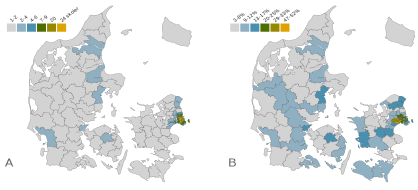
\includegraphics[width=1\linewidth]{images/figur_3_1} \caption{ Procentandel 0-16-årige inddelt efter ny inddeling.}\label{fig:fig-3-01}
\end{figure}

Det er primært G-gruppen (ikke-vestlig/ikke-vestlig), der er vokset i perioden. Børn og unge, hvor begge forældre er ikke-vestlige er steget fra 1,8 procent i 1985 til 10,4 procent i 2019. E-gruppen (vestlig-vestlig) er steget fra 0,4 til 2,3 procent. Men Figur \ref{fig:fig-3-01} viser også det stigende antal blandede børn.

\section{Herkomst og fremtidige partnerskaber}\label{herkomst-og-fremtidige-partnerskaber}

Hvordan de ''blandede børn'' klarer sig i skolen og videre på arbejdsmarkedet findes der nærmest ingen analyser af eftersom de har været usynlige i Danmark Statistisks kategorier. Men vi vil kort illustrere, hvordan en udvidet klassifikation kan give nye indsigter i integrationsprocesserne mellem indvandrere, efterkommere og danskere. Det gøres ved at se på partnerskaber i 2019 blandt den årgang, der var 16 år i 2009 (n=70482), dvs. dem der var 26 år i 2019. Af de 70.482 16-årige i 2009, var 32.081 samboende med en partner i 2019. I Tabel \ref{tab:tab-3-3} vises den andel blandt denne gruppe af unge, der har en partner med ''dansk herkomst``. Resultaterne for standardklassifikation vises i den øverste del af tabellen. Blandt gruppen med dansk-herkomst, der i 2019 levede i parforhold, havde 95 procent en partner, der også havde dansk herkomst. Den tilsvarende andel var 43 procent og 31 procent blandt indvandrere og efterkommere. Baseret på de resultater kunne man slutte, at danskerne næsten udelukkende danner par med andre danskere. Indvandrerne og efterkommerne danner hyppigst par med andre indvandrere og efterkommere, men blander sig dog mere op end det er tilfældet for danskerne.

\setlength{\LTpost}{0mm}
\begin{longtable}{lrr}
\toprule
Gruppe & \% & n \\ 
\midrule\addlinespace[2.5pt]
\multicolumn{3}{l}{Standardklassifikation} \\ 
\midrule\addlinespace[2.5pt]
Dansk herkomst & 95\% & 29967 \\ 
Indvandrere & 43\% & 697 \\ 
Efterkommere & 31\% & 1417 \\ 
\midrule\addlinespace[2.5pt]
\multicolumn{3}{l}{Udvidet klassifikation} \\ 
\midrule\addlinespace[2.5pt]
A: Dansk/dansk & 95\% & 27057 \\ 
B: Dansk/ukendt & 94\% & 1452 \\ 
C: Dansk/vestlig & 92\% & 852 \\ 
D: Dansk/ikke-vestlig & 85\% & 468 \\ 
E: Vestlig/vestlig & 86\% & 131 \\ 
F: Vestlig/ikke-vestlig & 60\% & 42 \\ 
G: Ikke-vestlig/ikke-vestlig & 25\% & 1604 \\ 
H: Øvrige & 63\% & 475 \\ 
\bottomrule
\end{longtable}
\begin{minipage}{\linewidth}
\emph{Note}: Partnerskab opgjort i registre via DST-standardklassifikation (E\_FAELLE\_ID).\\
\end{minipage}

Resultaterne for den udvidede klassifikation, vist i bunden af Tabel \ref{tab:tab-3-3} giver dog et mere nuanceret billede. Blandt dem med dansk-dansk-herkomst (A-gruppen) er det rigtigt, at majoritetsbefolkningen nærmest udelukkende danner par med majoritetsbefolkningen. Med vores udvidede klassifikation viser der sig også grupper af indvandrere/efterkommere, hvor partneren typisk er dansk. Det gælder for gruppen med vestlig/vestlig-herkomst (E), hvor andelen der har partnere med dansk-herkomst er oppe på 86 procent. Blandt gruppen med vestlig/ikke-vestlig baggrund er andelen på 60 procent. Igen er der tale om begrænsede, men voksende grupper. Det er således kun blandt gruppen med ikke-vestlig/ikke-vestlig herkomst, hvor det hyppigste er, at partneren ikke har dansk herkomst (se Qvist \& Qvist, -Qvist \& Qvist (\citeproc{ref-qvistqvist2023}{2023}), for nærmere analyse).

Mest interessant er det imidlertid, hvordan de blandede børn danner partnerskaber. Blandt gruppen med én dansk forældre og én vestlige forældre---der levede i parforhold---havde 92 procent en partner med dansk-herkomst. Blandt gruppen med én dansk forældre og én ikke-vestlig forældre var andel med partner med dansk herkomst på 85 procent. Det typiske er således, at de blandede børn finder partnere med dansk herkomst. Det er en indikation på, at de ''blandede børn'' ikke kun udfordrer ''os'' og ''dem'' klassifikationer, men også udviser en integrerende adfærd på ''partnerskabsmarkedet''.

\section{De blandede børn og integrationen}\label{de-blandede-buxf8rn-og-integrationen}

Partnerskabet er et tveægget sværd for integrationsprocesser. På den ene side er partnerskabet uden tvivl med til at dele et samfund op på tværs af skel; herunder etniske skel. Jo større de kulturelle forskelle er, jo mindre er sandsynligheden for at indgå i partnerskaber og giftmål, se det forrige kapitel. Denne drift mod kulturelt ensartede partnere var ét af vores argumenter for, at partnerskabet ikke var det mest centrale mødested for majoritet og minoritet. Jævnfør \hyperref[kap1]{kapitel 1} er ''problemet'' den høje grad af frivillighed i relationen. På den anden side etableres der en gang imellem tværetniske partnerskaber, der afstedkommer ''blandede'' børn, som har et stort potentiale til at nedbryde eksisterende ''os'' og ''dem'' kategoriseringer. I dette kapitel viste vi, hvordan gruppen af blandede børn har været støt voksende i Danmark siden 1985. I 2019 udgjorde de lidt over otte procent af alle 0--16-årige Danmark. Disse børn passer simpelthen ikke ind i vores eksisterende kategorier. Det er med til at gøre eksisterende etniske distinktioner uklare og formentlig udvide forståelse af hvad det vil sige at være dansk.

\chapter{Grundskoler som mødested}\label{kap4}

\emph{\href{https://vbn.aau.dk/da/persons/jeppefl}{Jeppe Fjeldgaard Larsen}}

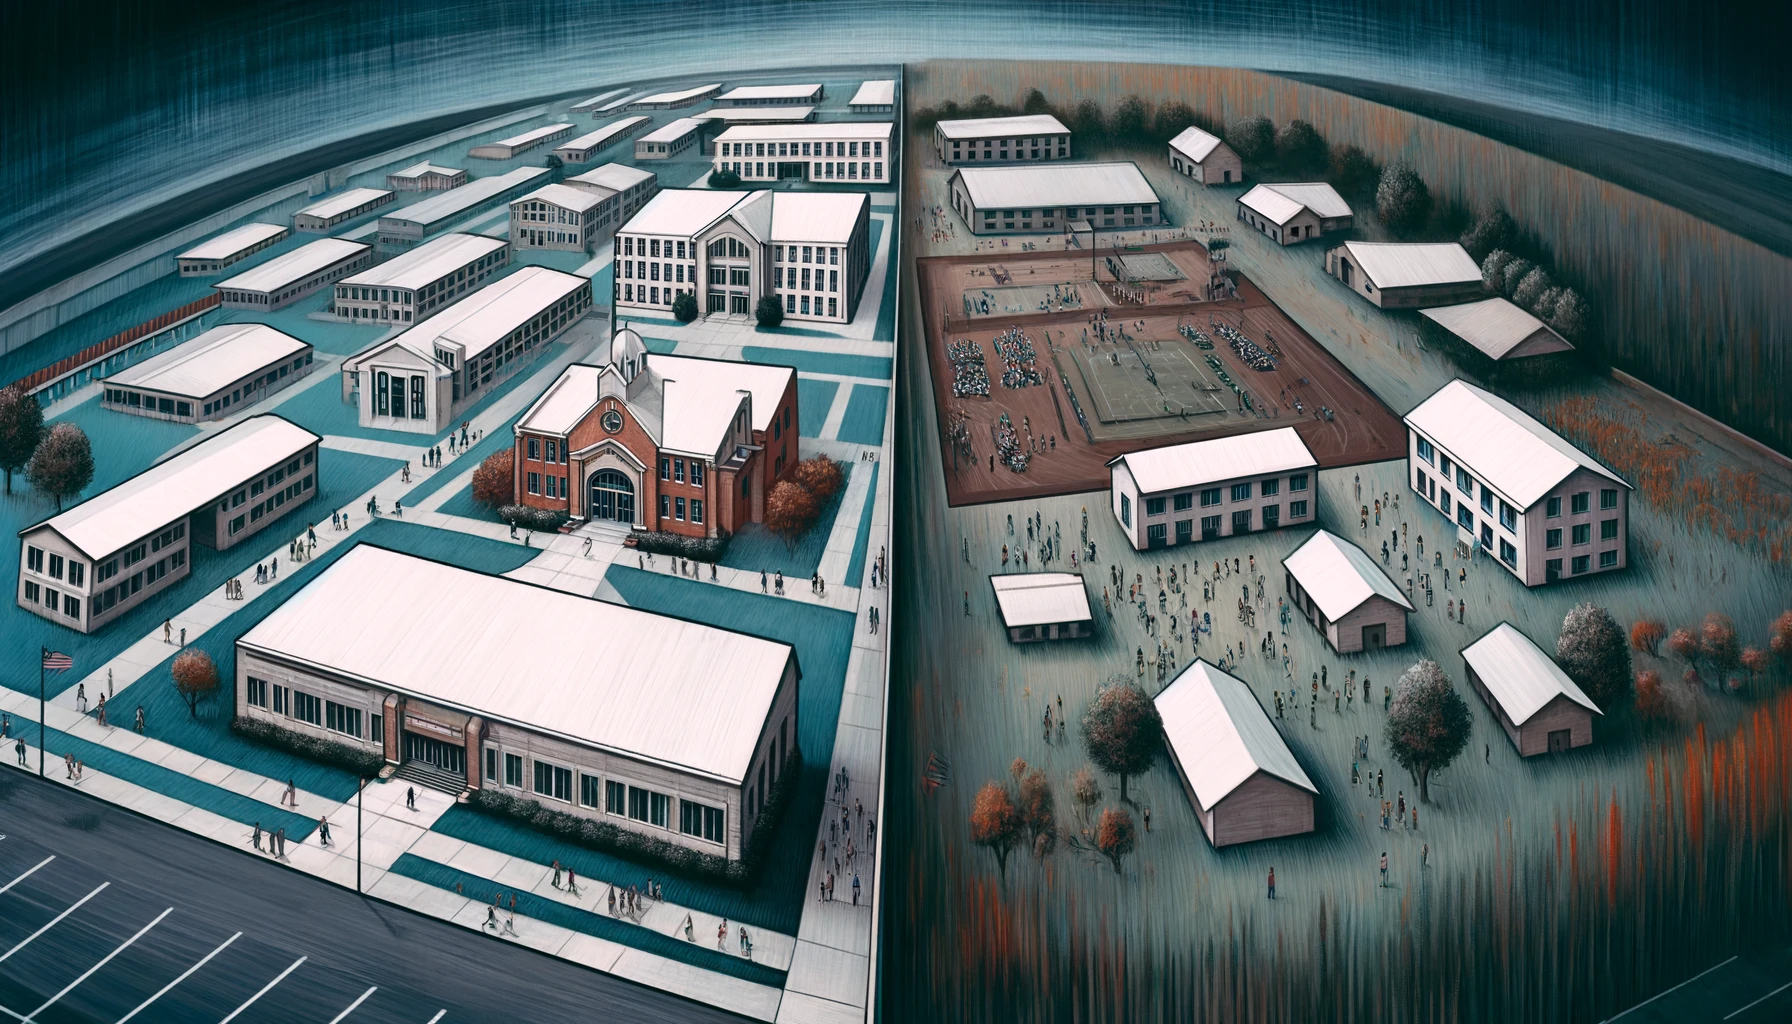
\includegraphics[width=1\linewidth]{images/dalle-schoolseg}

Jens Joel (MF, Socialdemokratiet) skriver i sin bog \emph{Fællesskaberen}, at ``tilliden, forståelsen og samhørigheden'' i Danmark er truet. Denne trussel mod den danske sammenhængskraft skyldes blandt andet, at vi ikke længere ``mødes {[}\ldots{]} i det, der før var `folkets skole'. I hvert fald ikke i tilstrækkelig grad'' (\citeproc{ref-joel2022}{Joel, 2002}, s. 11). Joel formår fortrinligt at tegne det grundlæggende solidariske og socialdemokratiske ideal for en fælles grundskole, hvor der er en tro på, at møder på tværs af forskellige baggrunde---hvad enten det er klasse eller etnisk tilhørsforhold---skaber tillid og tryghed i samfundet. I den socialdemokratiske forståelse af staten og samfundet er grundskolen dermed en helt fundamental ``byggesten i samfundet'' (Ibid., s. 11), fordi grundskolen er en institution, hvor børn kan interagere med hinanden, uanset deres ligheder med andre børn og deres forældre.

Men hvornår nåede (eller når) skolesegregeringen et niveau, hvor den ligefrem truer sammenhængskraften i vores samfund? Selvom noget forskning har forsøgt empirisk at definere den ''optimale sammensætning'' af børn i en klasse er ift. læring og sociale relationer (se nedenfor) eller ''tipping points'' for, hvornår etnisk danske familier fravælger den lokale skole på grund af en oplevelse af for stor andel minoriteter, er det i høj grad et politisk spørgsmål, hvornår segregering er ''for højt''. Faktum er imidlertid, at der er kommet flere ''minoritetsskoler'', hvor ingen---eller kun en mindre andel---børn med dansk oprindelse går i skole. Hvilket samtidigt betyder at der fortsat også er mange skoler, hvor ingen børn med indvandrerbaggrund går i skole. Det er sådanne ulige fordelinger af børn mellem skoler, vi forstår som skolesegregering. Selvom disse ''absolut segregerede'' skoler eksisterer, er skolesegregering typisk et spektrum af ulige fordeling af børn mellem skoler. Tag et stiliseret eksempel: I et område med tre skoler, hvor \(15\%\) af alle børn har indvandrerbaggrund. Én af skolerne har en andel af børn med indvandrerbaggrund på \(50\%\), mens de andre skoler har en andel på \(5\%\). Dette ville vi karakterisere som et segregeret område, da graden af eksponering mellem majoritets- og minoritetsgrupperne på skolerne ikke afspejler den eksponering, der ville være forventet givet befolkningssammensætningen. Konkret har Socialdemokratiet fremsat en ambition om, at ingen skoler skal have en andel af børn med \emph{ikke-vestlige} baggrunde over \(30\%\).

Selvom skæringspunktet på \(30\%\) tidligere er blevet fremhævet som et ``tipping point'' for, hvornår etnisk danske familier fravælger den lokale skole og igangsætter selvforstærkende segregeringsprocesser (\citeproc{ref-rangvid2010}{Rangvid, 2010}), vil jeg ikke tage stilling til eller give svar på, hvornår segregering er problematisk---og om det i alle situationer er ikke-ønskværdigt. I stedet vil jeg med dette kapitel empirisk beskrive grundtrækkene i omfanget af skolesegregering i den danske grundskole fra 1985 til 2020 som et bidrag og afsæt til videre debat.
Som jeg vil beskrive i det følgende, tenderer den store forfaldshistorie om et samfund, der ikke hænger sammen (i en kontekst af grundskolen), mod det overdrevne. Vi ser nemlig, at segregering generelt har været forholdsvis konstant og måske ikke så stærk som man kan få indtryk af i den offentlige debat. Men det er samtidigt også klart, at der er et stigende antal skoler, hvor børn med etnisk dansk baggrund udgør et numerisk mindretal, på trods af at børn med indvandrerbaggrund kun udgør \(12\%\) af alle børn i skolealderen i 2020, om end dette drejer sig om \(33\) skoler ud af \(1468\), hvor mere end halvdelen af eleverne har ''ikke-vestlige baggrunde''. Disse skoler er dog ikke tilfældigt fordelt, men placeret i bestemte kommuner og nabolag, der også er kendetegnet ved en relativt høj grad af boligsegregering. Med andre ord, selvom den store forfaldsfortælling måske ikke holder, er der stadig på lokale niveauer inden for kommuner i bestemte områder, hvor der kan være grund til bekymring og selvforstærkende segregeringsprocesser. En central pointe er, at den videre debat derfor må skelne mellem to dimensioner: Den store nationale skala, som måske kan bidrage til en meget generel fortælling om samfundstilstanden i Danmark, og den kommunale skala, hvor lokale og specifikke processer finder sted, men som ikke nødvendigvis kan generaliseres til at udtrykke en samfundsdiagnose.

Selvom skolesegregering på mange måder er et velbeskrevet fænomen i den internationale litteratur (se J. F. Larsen (\citeproc{ref-larsen2024a}{2024a}) for et overblik), er disse beskrivelser ofte grovkornede, da de er baseret på aggregerede tabeldata. Det betyder, at beskrivelserne er lavet på data, der er aggregeret på en høj geografisk eller administrativ skala, hvilket gør det umuligt at sige noget om relationen mellem de enkelte familiers sociale status eller hvilket skoledistrikt, de bor i, og graden af segregering. Med de danske registerdata er det muligt at lave en detaljeret og mere finkornet beskrivelse af fordelingen af børn mellem skoler, da disse data indeholder detaljeret information om hvert enkelt barn i alle skoler, inklusive privat- og friskoler, hvilket også sjældent er tilgængeligt i den internationale segregeringslitteratur. For eksempel kan vi detaljeret undersøge sammenhængen mellem bosætningsmønstre og tendenser i skoleindskrivninger. Med disse beskrivelser er det hensigten at nuancere og kvalificere de pågående debatter vedrørende den danske grundskole og dens rolle i de danske målsætninger for integration.

Kapitlet er opdelt i seks sektioner. Første sektion skitserer den danske kontekst og de centrale tematikker i skolesegregeringslitteraturen. Anden sektion præsenterer det danske skolelandskabs geografi og demografi. Tredje sektion måler graden af segregering på både nationalt og kommunalt niveau. Dette efterfølges af en præsentation og diskussion af, hvordan skolesegregering skal ses som et produkt af boligsegregering i sektion fire. Femte sektion beskriver og diskuterer, hvordan observerede grader af segregering skal tolkes i relation til faktiske møder mellem børn fra forskellige baggrunde. Sjette og sidste sektion konkluderer.

\section{NY OVERSKRIFT}\label{ny-overskrift}

I den internationale kontakt- og integrationslitteratur fremhæves skoler ofte som steder med potentiale til at nedbryde fordomme og stereotyper. Det vil sige, at kontakt i en skolekontekst på daglig basis kan være med til at skabe gensidig forståelse og konfrontere uberettigede fordomme og stereotyper mellem grupper, fordi børn får mulighed for at møde og se hinanden som individer fremfor som medlemmer af grupper. Dette potentiale for at nedbryde fordomme og stereotyper er dog ifølge teorien betinget af fire forhold, for at kontakt mellem grupper faktisk har en produktiv og positiv konsekvens : 1) Børnene befinder sig i en kontekst, hvor der er en autoritet (læreren), der strukturerer interaktioner og opgaver. 2) Børnene forventes at have et fælles mål (læring/eksamener). 3) De arbejder sammen om dette mål i overensstemmelse med skolens didaktiske principper. 4) Børnene har samme status i klassen (alle er elever underlagt læreren) (\citeproc{ref-pettigrew2006}{Pettigrew \& Tropp, 2006}; \citeproc{ref-tropp2005}{Tropp \& Pettigrew, 2005}; \citeproc{ref-allport1979}{\textbf{allport1979?}}). Det skal dog ikke underkendes, at der både er forskning og personlige historier, der beskriver tilfælde af diskrimination og fordomme mellem lærer og minoritetselever og elever imellem (\citeproc{ref-andersen2019}{S. C. Andersen \& Guul, 2019}). Lige status er derfor ikke nødvendigvis givet i en skolekontekst. Optimal kontakt i denne kontekst, som påpeget af Pettigrew (\citeproc{ref-pettigrew1998}{1998}), er ydermere betinget af, 5) at interaktionerne har venskabspotentiale. Da børn i en klasse har samme alder, og der som regel er en nogenlunde lige kønsfordeling i de fleste skoler, er der et principielt højt venskabspotentiale i de danske grundskoler (\citeproc{ref-mcpherson2001}{McPherson et al., 2001}).

International forskning har vist, at børn i såkaldte ``blandede skoler'', hvor elevsammensætningen ligner den egentlige befolkningssammensætning, har flere venskaber eller sociale relationer på tværs af etniske gruppeskel (\citeproc{ref-kruse2019}{Kruse \& Kroneberg, 2019}; \citeproc{ref-leszczensky2015}{Leszczensky \& Pink, 2015}). En anden forventet effekt er de såkaldte klassekammerateffekter (peer effects), som antager, at ressourcestærke elever kan være med til at hæve det faglige niveau for deres mindre ressourcestærke klassekammerater. Der pågår dog samtidigt diskussioner om, at både kontakt- og klassekammerateffekter i en metodologisk forstand er svære at isolere kausalt, da der forventeligt er grundlæggende problemer med selvselektion. For eksempel vil familier med de allerede laveste fordomme være mere tilbøjelige til at vælge den etnisk diverse distriktsskole (se f.eks. Hassan et al. (\citeproc{ref-hassan2022}{2022}) eller Hermansen \& Birkelund (\citeproc{ref-hermansen2015}{2015}) for en oversigt og diskussion).

\subsection{Den danske grundskole}\label{den-danske-grundskole}

Grundskolen i Danmark omfatter børn i alderen 6-16 år. Et særligt kendetegn ved den danske grundskole, sammenlignet med andre internationale skolesystemer, er fraværet af \emph{tracking}---også kaldet elevdifferentiering eller klasseopdeling---baseret på faglige evner. Det betyder, at børn ikke bliver placeret på bestemte skoler eller spor afhængigt af deres præstationer i de tidlige skoleår, som det er tilfældet i andre europæiske lande som Tyskland, Holland og England. I stedet fastlægger folkeskoleloven, at undervisningen i det danske skolesystem skal tilpasses det pågældende klasserum gennem undervisningsdifferentiering, målrettet klasserummet som det er fra børnehaveklassen frem til afgangseksamen i alle fag. Med det danske princip om undervisningsdifferentiering i stedet for elevdifferentiering er den danske grundskole dermed forventeligt et eksempel på optimal realisering af positive kontakt-effekter gennem sociale relationer på tværs af gruppetilhørsforhold i et barns formative år (\citeproc{ref-larsen2016}{C. A. Larsen, 2016}; \citeproc{ref-larsen2024c}{J. F. Larsen, 2024b}), når børnene tilbringer 10 år sammen i alle fag. Den aktuelle udfordring er imidlertid, at Danmark har en meget liberal og generøs skolevalgspolitik, hvor omkring 75\% af omkostningerne for hvert enkelt barn på en privatskole er statsfinansierede, mens den resterende fjerdedel er brugerbetaling. Dette gør privatskoler tilgængelige for en stor del af befolkningen---men samtidig utilgængelige for de laveste indkomstgrupper. Dette har skabt bekymringer for, at det socialdemokratiske princip om, at børn fra forskellige baggrunde går på samme skole, ikke længere bliver realiseret, fordi forældre frit kan vælge skoler til og fra.

Historisk set går retten til at bestemme over sit barns skolegang, under myndighedernes tilsyn, tilbage til Friskoleloven fra 1855. Selvom hver adresse er tilknyttet et skoledistrikt, hvor barnet har garanteret ret til indskrivning, tillader reglerne i dag, at familier frit kan søge om indskrivning på en anden folke-, privat- eller friskole, enten inden for kommunen eller i en anden kommune. Det eneste lovlige grundlag, en folkeskole kan afvise et barns optagelse på, er, hvis skolen ikke har plads, hvilket defineres som 28 børn i hver klasse i den pågældende årgang. Kommuner kan dog sænke den maksimale klassestørrelse til under 28 elever for at begrænse mulighederne for anvendelsen af skolevalg.

Til forskel kan fri- og privatskoler permanent bortvise børn eller afvise optagelse baseret på en individuel vurdering, hvilket folkeskoler også kunne før 2005. Grundet den decentrale finansiering af folkeskolen har de enkelte folkeskoler også store individuelle omkostninger ved at flytte et barn til et specialtilbud. I modsætning hertil har privatskolerne mindre udgifter i forbindelse med henvisninger til specialtilbud, idet de søger disse midler hos staten, hvor folkeskolerne skal finde midlerne i deres kommunalt allokerede budget.

Disse strukturelle forhold har affødt en grundlæggende bekymring for, at frit skolevalg og det private skolemarked vil føre til stigende ulighed og segregation mellem skoler på grund af socioøkonomiske forskelle i, hvem der i størst omfang vælger -- eller er i stand til -- at benytte sig af muligheden for frit skolevalg ved skolestart eller i løbet af barnets skolegang.

\subsection{Betingelser for møder i grundskolen}\label{betingelser-for-muxf8der-i-grundskolen}

Den primære hindring for realiseringen af kontakt- eller klassekammerateffekter i barndommen er først og fremmest omfanget af skolesegregering, da det konkret forhindrer kontakt mellem grupper af børn, hvis de ikke møder hinanden i deres daglige liv (\citeproc{ref-kruse2017}{Kruse, 2017}). Grundlæggende er segregering er et udtryk for en fysisk adskillelse af personer fra forskellige klassificerede grupper. Disse grupper kan være defineret ud fra majoritets-/minoritetsstatus, social status, køn og andre former for identitets-, økonomiske eller sociale faktorer. Typisk er segregering blevet diskuteret i forhold til (etnisk) boligsegregering, som angiver i hvilket omfang personer med indvandrerbaggrund bor i de samme boligområder som personer med dansk oprindelse---og omvendt. På samme måde udtrykker etnisk skolesegregering i hvilket omfang børn med dansk oprindelse kun (eller primært) går på skoler med andre børn med dansk oprindelse, og \emph{vice versa}. En vigtig pointe her er, at segregering refererer til fordelingen eller spredningen af de \emph{to} grupper, der sammenlignes. Det vil sige, at minoritetsgruppen ikke kan være segregeret uden at majoritetsgruppen også er det.

I Larsen (\citeproc{ref-larsen2024b}{2024c}, \citeproc{ref-larsen2024c}{2024b}) viser jeg, at det særligt er mekanismer på boligmarkedet, der driver skolesegregering, snarere end aktivt til- og fravalg af bestemte skoler, som ellers er den meget omtalte diagnose i den offentlige debat. For det første observerer vi, at børnefamilier gradvist bliver mere segregerede bosætningsmæssigt fra barnets fødsel indtil barnet begynder i børnehaveklassen. Dette indikerer, at familier, når eller hvis de flytter med børn i førskolealderen, er tilbøjelige til at bosætte sig i nabolag, hvor de andre beboere ligner dem selv. Samtidig ser vi, at når først barnet er startet i skole, er familier mindre tilbøjelige til at flytte, før barnet har afsluttet grundskolen (\citeproc{ref-larsen2024c}{J. F. Larsen, 2024b}). Disse bosætningsmønstre er centrale for at forstå skolesegregering i Danmark, da både nabolaget og skoledistriktet, som en familie bor---eller bosætter sig---i, hænger stærkt sammen med elevsammensætningen på den skole, som barnet går i (\citeproc{ref-larsen2024b}{2024c}). Dette forklares ved den simple observation, at mulighederne for at udnytte det frie skolevalg er betinget af de skoler, der er i nærheden af bopælen. Med andre ord betinger familiens bopæl deres reelle muligheder på skolemarkedet og er af større betydning end sociale gradienter i, hvilke familier der vælger privat- og friskoler (\citeproc{ref-larsen2024a}{J. F. Larsen, 2024a}; \citeproc{ref-bjerrenielsen2020}{\textbf{bjerrenielsen2020?}}). I et kausalitetsperspektiv betyder dette selvfølgelig, at vi ikke kan udelukke betydningen af skolevalget i en omvendt sammenhæng, idet valg af bolig også (in)direkte er et valg af skoledistrikt.

\section{Det danske skolelandskab}\label{det-danske-skolelandskab}

Når vi ser på det fysiske skolelandskab, det vil sige alle skoler og deres adresser, var det danske skolelandskab i 1985---det tidligste år, vi har data---bestående af 1327 skoler, hvoraf 246 var privat- eller friskoler. I 2020---det seneste år, vi har data for---var der samlet 1848 individuelle skoler, hvoraf 545 var privat- eller friskoler. Denne optælling ser bort fra alle specialtilbud, efterskoler og lignende og inkluderer kun institutioner, der i institutionsregistret er klassificeret som folkeskole eller privat- og friskole. I 2020 havde \(12\%\) af alle børn i niende klasse enten første eller anden generation indvandrerbaggrund. Til sammenligning var det kun under \(2\%\) i 1985.

Fra et geografisk perspektiv er der stor variation i, hvor tæt skoler ligger på hinanden. Dette har en indirekte betydning for omfanget af frit skolevalg, da områder med få skoler inden for relativt kort afstand også har færre reelle muligheder for at vælge alternative til distriktskolen, som diskuteret ovenfor. Figur \ref{fig:fig-3-1} visualiserer antallet af skoler inden for \(2 km\) fra det geografiske centrum af bopælssognet.

Kortet fungerer på sin vis som en indikator for befolkningstæthed, da der naturligvis vil være flere skoler i områder med mange familier. Men på grund af lave omkostninger ved etablering af private- eller friskoler vil nogle områder stadig have et relativt stort skolemarked, på trods af relativ lav befolkningstæthed. For at åbne en fri- eller privatskole er den eneste ikke-refunderbare direkte omkostning et gebyr på 20.000 kr. til ministeriet i forbindelse med anmeldelse om oprettelse af ny skole. Derfor gælder det, at familier i urbane områder generelt har flere skoler, de potentielt kan vælge mellem. De fleste husstande i Danmark har to skoler inden for en realistisk pendleafstand på \(2 km\), men som bemærkelsesværdige afvigelser fra gennemsnittet er der i København og Frederiksberg henholdsvis \(20\) og \(24\) skoler inden for \(2 km\).

\begin{figure}
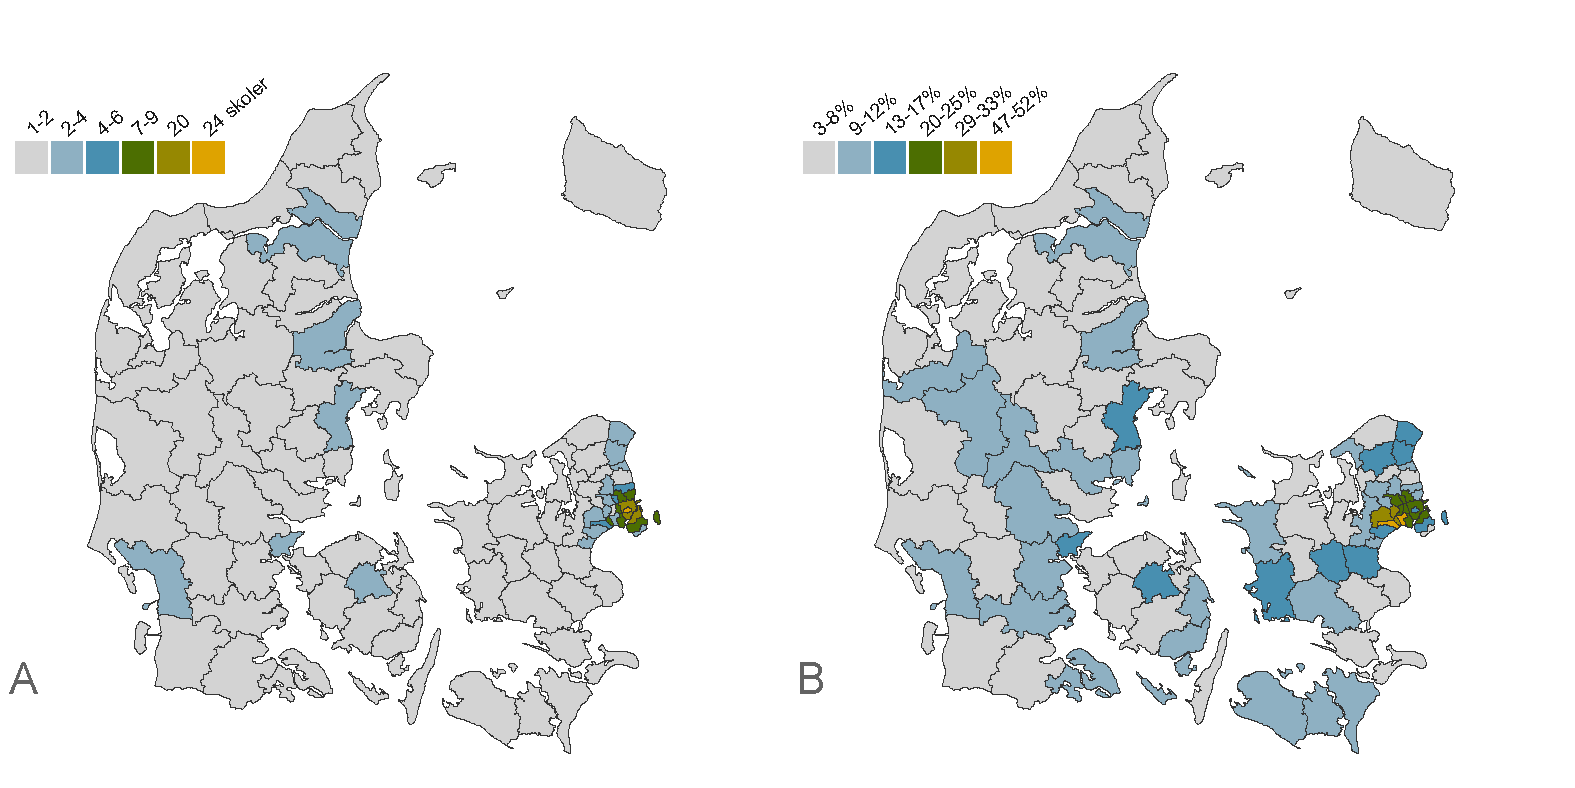
\includegraphics[width=1\linewidth]{images/figur_3_1c_distance_antal} \caption{Gennemsnitligt antal skoler inden for 2 km af bopælsadressen (A) og koncentration af børn med ikke-vestlig indvandrerbaggrund i skolealderen i 2020 (B). <br> <br> Note: * Afstandene til skolen er baseret på den euclidiske afstand fra bopælssognets centroid til de geografiske koordinater for skolens adresse. Ikke-vestlig indvandrerbaggrund inkluderer børn, hvor begge eller én af forældrene er første generations immigrant fra et ikke-vestligt land.*}\label{fig:fig-3-1}
\end{figure}

Det centrale her er, at fordi børnefamilier med indvandrerbaggrund er koncentreret i urbane områder (se \hyperref[kap1]{kapitel 1}), er konsekvensen en stærk korrelation mellem store skolemarkeder (områder med mange skoler at vælge mellem) og områder med høj etnisk diversitet. Figuren giver dermed et deskriptivt indblik i, hvordan det fysiske skolelandskab og demografiske forhold kan spille sammen. I urbane områder, såsom hovedstadsområdet, er der en høj koncentration af skoler, hvilket giver mange muligheder for skolevalg. Samtidig er der også en højere koncentration af børn med indvandrerbaggrunde, særligt fra ikke-vestlige baggrunde. Dette skaber et potentiale for både høj etnisk diversitet i skolerne og for etnisk skolesegregering, da familier har mulighed for at vælge skoler væk fra dem med høj andel af elever med ikke-vestlig baggrund. I forstæderne og mindre byer er der færre skoler, hvilket betyder flere strukturelle begrænsninger for skolevalg. Samtidig er koncentrationen af familier med indvandrerbaggrund tilsvarende lavere. I kontrast er der i landdistrikterne få skoler inden for pendleafstand fra bopælen og dermed begrænsede muligheder for skolevalg. Her er koncentrationen af familier med ikke-vestlige baggrunde meget lav, hvilket forventeligt leder til lav diversitet på skolerne og en høj grad af strukturelt betinget skolesegregering grundet en lille minoritetsgruppe. Sammenfattende illustrerer figuren hvordan forholdet mellem strukturelle betingelser givet ved det fysiske skolelandskab og demografiske forhold mellem forskellige geografiske områder kan påvirke mulighederne for skolevalg og niveauet af etnisk diversitet i skolerne, og understreger de strukturelle forhold, der kan føre til skolesegregering.

Med andre ord, i urbane områder er der på den ene side et strukturelt potentiale for ``blandede'' skoler med høj gensidig eksponering mellem majoritets- og minoritetsgrupper, fordi der er en relativ høj koncentration af familier med indvandrerbaggrunde. Det vil sige, at de fleste familier med dansk oprindelse har en stor sandsynlighed for at møde andre familier, der ikke ligner dem selv. Samtidig er der dog også et stort strukturelt potentiale for etnisk skolesegregering, der overstiger det niveau, som er betinget af etnisk boligsegregering. Dette skyldes, at der er nok skoler til, at familier realistisk kan undgå de mindre attraktive skoler ved at indskrive deres børn på andre skoler (\citeproc{ref-larsen2024b}{J. F. Larsen, 2024c}). Disse mindre attraktive skoler er---rimeligt eller ej---ofte associeret med en høj andel elever fra ikke-vestlige immigrantbaggrunde. De fleste familier angiver, når de bliver spurgt, at det vigtigste kriterium i skolevalget er barnets trivsel og skolens ``faglige kvalitet'' (\citeproc{ref-epinion2017}{Epinion, 2017}). Denne kvalitet kan dog ofte være svær at vurdere i praksis, så det udefra observerbare elevgrundlag bliver ofte en målestok for vurderet kvalitet og skolens omdømme (\citeproc{ref-rambuxf8ll2011}{Rambøll, 2011}). Empiriske studier viser, at familier med de højeste uddannelser også er mest sensitive over for antallet af ``ikke-indfødte'' elever på en skole (\citeproc{ref-karsten2003}{Karsten et al., 2003}; \citeproc{ref-bjerrenielsen2020}{\textbf{bjerrenielsen2020?}}; \citeproc{ref-nielsen2019}{\textbf{nielsen2019?}}). Efter trivsel og ``faglig kvalitet'' er ``afstand til skolen'' fra bopælen også et vigtigt kriterium for mange forældre (\citeproc{ref-epinion2017}{Epinion, 2017}). Derfor kan sammenhængen mellem antallet af skoler og koncentrationen af børn med ikke-vestlig indvandrerbaggrund være med til at forstå de udfordringer og muligheder, der eksisterer for integration og skolevalg i forskellige geografiske områder. Urbane områder med mange skoler og høj diversitet står over for udfordringen med at sikre, at kontakt- og klassekammerateffekter kan realiseres på grund af segregeringsprocesser, mens landdistrikter kan være udfordret af begrænsede skolevalgmuligheder.

\section{Segregering i det danske skolelandskab}\label{segregering-i-det-danske-skolelandskab}

Når vi måler graden af segregering, er det mest anvendte mål for (skole)segregering \emph{Dissimilarity} (\(D\)) indekset, men også \emph{Separation} (\(S\)) indekset har en vis udbredelse . Begge mål kan have værdierne 0-1, og i empiriske cases vil de to mål essentielt altid være korrelerede. \(S\) er typisk noget lavere end \(D\), da \(S\) korrigerer for størrelsen af skoler og grupper, mens \(D\) ikke gør (se \hyperref[bilag1]{bilag A} for yderligere information). Den grundlæggende forskel mellem de to mål er, at \(D\) måler graden af ulige fordeling, mens \(S\) måler graden af polarisering.

Lidt simplificeret vil det sige, at \(D\) måler, hvor mange fra én af grupperne i sammenligningen, der hypotetisk skal flyttes til en ny skole for, at fordelingen er ``lige''. ``Lige fordeling'' er i denne kontekst et udtryk for en situation, hvor samtlige skoler i en kommune/nation har samme andel minoriteter som på kommunalt/nationalt niveau. Det vil sige, at indekset måler i hvilket omfang andelene på de enkelte skoler ligner den overordnede befolkningssammensætning i området. Et lavt \(D\)-indeks udtrykker altså, at alle eller de fleste skoler har en andel af hver gruppe, der spejler størrelserne af grupperne i populationen. Modsat udtrykker et højt \(D\)-indeks, at få skoler optager næsten alle minoriteter og vice versa. For eksempel, i et område med tre skoler og en population, hvor \(15\%\) har indvandrerbaggrund, skal alle skoler have en andel på \(15\%\) for ingen segregering, hvilket svarer til \(D=0\). Indekset skelner dog ikke til de absolutte tal, så om \(15\%\) udgøres af \(15\) ud af \(100\) elever eller \(150\) ud af \(1000\) gør ingen forskel i indekset. I en substantiel og levet kontekst er det selvfølgelig af betydning.

Med det samme eksempel for den hypotetiske kontekst er størrelsen af skolerne af betydning for målet for \(S\), idet det udtrykker hvilket omfang børn fra forskellige baggrunde er isoleret fra hinanden. Hvis én skole har en andel elever med indvandererbaggrund på \(15\%\) og de andre to har \(5\%\) og alle skoler har en størrelse på 25 elever, vil \(S \approx 0,05\). Hvis elevtallet var \(100\) på skolen med en andel på \(15\%\) og fortsat 25 på de to andre skoler ville \(S \approx 0,025\), da flere børn fra den samlede majoritetsgruppen vil være eksponeret til børn med indvandrerbaggrund. \(S\) er derfor en kvantifisering af den gennemsnitlige eksponering til ens egen gruppe (eller isolering fra sin udgruppe), kontrolleret for den relative størrelse af grupperne, da en lille minoritetsgruppe kan være isoleret som en ren tilfældighed, mens en relativ stor minoritetsgruppe som er isoleret, vil som udgangspunkt være et udtryk for en systematisk sortering og ikke en tilfældighed. Med andre ord, hvor stor en andel børn med dansk oprindelse går det gennemsnitlige barn med dansk oprindelse i skole med---og omvendt for børn med indvandrerbaggrund. Det er derfor grundlæggende et mål for gennemsnitlig eksponering til sin egen gruppe mod eksponering til en anden gruppe. \(S=0\) udtrykker en fordeling mellem skoler, hvor børn på alle skoler har den samme grad af intergruppe eksponering. Derfor, og igen en smule simplifiseret skal \(S\), tolkes som omfanget af eksponering mellem to grupper og kan dermed også tolkes som et spektrum af polarisering mellem to grupper.

\subsection{National skala}\label{national-skala}

På landsplan måles segregeringen til \(D = 0,44\) og \(S = 0,16\) i 2020, se Figur \ref{fig:fig-3-2}. Som diskuteret indledningsvis, præcis hvornår segregering er ``for høj'' er delvist et politisk og normativt spørgsmål. Dog peger den klassiske (amerikanske) segregeringslitteratur på, at \(D<0,3\) anses som lavt, mens \(D>0,6\) betragtes som højt (\citeproc{ref-massey1994}{D. S. Massey \& Denton, 1994}). I en segregeringskontekst vil \(S=0,6\) betragtes som meget højt, da der vil være en betydelig mængde skoler, der (næsten) udelukkende består af enten majoritets- eller minoritetsbaggrund, og den gennemsnitlige eksponering til ens egen gruppe er markant større end den ville være under forudsætning af tilfældige fordelinger mellem skoler. Nedenfor i Figur \ref{fig:fig-3-2} ses udviklingen af begge mål for segregering. Grundlæggende har graden af skolesegregering på begge dimensioner været nogenlunde stabil siden starten af 00'erne. Bemærk, at som det er diskuteret ovenfor, er to grundlæggende forskellige dimensioner af fordeling af børn, der måles. Vi ser derfor, at de to mål for segregering tilsyneladende konvergerer frem mod 00'erne. Dette skyldes ændrede strukturelle forhold. Simpelt sagt, i 1985 var der for få børn med indvandrerbaggrund og for mange skoler til, at disse børn kunne have været ``ligeligt'' fordelt i henhold til \(D\)-indekset. En vis grad af skolesegregering har derfor været en strukturel betingelse. Til gengæld viser \(S\)-indekset, at denne gruppe af børn med indvandrerbaggrund i meget stort omfang har gået på skoler, hvor de har udgjort en numerisk minoritet. Igen en strukturel betingelse, når minoritetsgruppen udgør en lille gruppe i numerisk forstand. Gruppen har ikke været stor nok til, at den i praksis kunne have udgjort en numerisk majoritet på enkelte skoler. I takt med at gruppen af børn med indvandrerbaggrund bliver større relativt til gruppen af børn med dansk oprindelse, er der altså de nødvendige strukturelle betingelser for, at flere---hvis ikke de fleste---skoler kan optage børn med indvandrerbaggrund. Dette bliver til en vis grad realiseret. Men, som vi ser med et parallelt stigende \(S\)-indeks, kommer der fortsat flere skoler, hvor børn med indvandrerbaggrund udgør en relativt stor andel eller den numeriske majoritet på skolen. Dette har en klar strukturel tolkning. Indvandrerfamilier bosætter sig disproportionelt i hovedstadsområdet og de største kommuner (se se \hyperref[kap1]{kapitel 1}), hvilket muliggør eksistensen af skoler, hvor størstedelen udgøres af børn med indvandrerbaggrund. Konvergeringen, hvor det ene mål falder og det andet stiger, tolkes derfor som primært at være drevet af ændrede strukturelle betingelser for segregering---herunder historiske bosætningsmønstre blandt familier med indvandrerbaggrund.

\begin{figure}
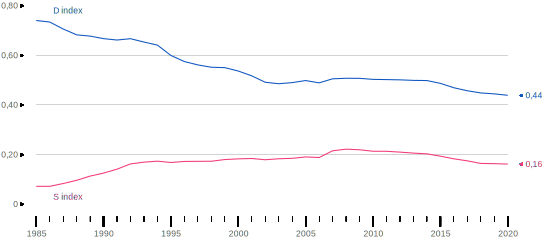
\includegraphics[width=1\linewidth]{images/figur_3_2} \caption{Etnisk skolesegregering i Danmark}\label{fig:fig-3-2}
\end{figure}

Graden af segregering i Danmark vil derfor være at betragte som moderat i dag, hvilket kan være overraskende for nogle, givet den aktuelle offentlige debat, hvor man kunne tro, at den har været voldsomt stigende. På nationalt plan har segregeringen faktisk været faldende. Selvom fordelingen har været skæv, især frem til årtusindskiftet, har der ikke været egentlig polarisering, hvor minoritetsgrupper har gået på skoler med meget begrænset kontakt til majoritetsgrupper. Med andre ord, graden af segregering (\(D\)) har tidligere grundlæggende været strukturelt betinget, idet der ikke har været tilstrækkeligt mange minoritetsbørn, og de har været koncentreret i for få kommuner til, at de praktisk kunne fordeles blandt alle skoler i Danmark. Fordelingen af denne gruppe børn ville altså være skæv, selv ved en tilfældig fordeling af børn mellem skolerne. Samtidig har vi dog set en stigning i \(S\)-indekset frem til omkring 2007. Denne stigning skal særligt ses i lyset af bosættelsesmønstrene blandt immigranter. Når visse kommuner oplever en relativ koncentration af immigranter, vil der i numerisk forstand være ``nok'' børn med indvandrerbaggrund til at udgøre en større andel af elevgrundlaget på en skole. Især fremkomsten af muslimske friskoler bidrager til polarisering i en segregeringskontekst, især når der samtidig også er skoler, hvor alle børn har dansk oprindelse. I en substantiel tolkning kan denne grad af segregering oversættes til faktisk intergruppe eksponering. Det vil sige, for det \emph{gennemsnitlige} barn med indvandererbaggrund, hvor stor en andel af den potentielle sociale gruppe på en grundskole har indvanderernaggrund, og \emph{vice versa}? I 1985, har det gennemsnitlige barn med indvandererbaggrund en \emph{potentiel} eksponering til børn andre børn med indvandererbaggrunde på deres skole på \(16\%\). I 2020, er denne \emph{potentielle} eksponering steget til \(35\%\). For det gennemsnitlige barn med dansk oprindelse, var eksponeringen til børn med indvandererbaggrunde \(7\%\) i 1985 og \(19\%\) i 2020.

\subsection{Lokal skala}\label{lokal-skala}

Når segregering måles på en stor skala, som f.eks. på landsplan, skjules betydelige lokale variationer i gennemsnittet. I Figur \ref{fig:fig-3-3} er begge mål for segregering og deres korrelation illustreret. Figuren skal læses således, at segregering kan være lav/høj målt som \(D\) (rødlige farver: horizontale kvadranter) eller lav/høj målt som \(S\) (blålige farver: vertikale kvadranter). Idet de to mål ofte korrelerer i praksis, ser vi også, at de to mål for segregering ofte er lav/lav eller høj/høj på begge dimensioner (lilla farver: diagonale kvadranter fra nedre-venstre til øvre-højre). Disse lokale variationer viser, at selvom landsplan-data kan indikere en moderat segregering, kan der være betydelige forskelle mellem kommuner. Nogle kommuner kan have høj polarisering uden en ulige fordeling af elever på skolerne, mens andre kan have en ulige fordeling uden stærk polarisering. Dette illustrerer vigtigheden af at analysere segregering på forskellige geografiske niveauer for at få et mere nuanceret billede af situationen.

Ved at måle skolesegregering i de enkelte kommuner over tid, med fokus på år 1985 og 2020, ser vi i 1985, at segregeringsniveauet lå mellem \(D=0,2-0,4\) i nogle kommuner, mens det i andre kommuner var over \(D>0,4\). Det er dog væsentligt at bemærke, at ingen af disse kommuner havde høj segregering, hvis det måles som polarisering (\(S\)). Alle kommuner havde et segregeringsniveau under \(0,1\) målt som \(S\) i 1985. Tolkningen af disse to dimensioner af segregering i sammenhæng er derfor, at selvom der isoleret set var relativt høje grader af segregering i flere kommuner i 1985, skyldtes dette i høj grad strukturelle forhold, som diskuteret ovenfor. Med andre ord, selvom \(D\)-indekset viste en ulige fordeling af elever med indvandrerbaggrund, viste \(S\)-indekset, at der ikke var en høj grad af polarisering, hvilket betyder, at eleverne stadig havde en vis grad af kontakt på tværs af grupper.

Dette ændrer sig dog frem mod 2020, hvor vi ser, at mange kommuner har både en høj grad af ulige fordeling af minoritetsbørn mellem skoler (\(D\)) og at børn med indvandrerbaggrund udgør en betydelig del af elevgrundlaget på bestemte skoler (\(S\)) og vice versa for børn med dansk oprindelse. Med andre ord, segregering målt som henholdsvis \(D\) og \(S\) begynder at korrelere stærkere over tid, hvilket betyder, at skolesegregeringen i mange kommuner i dag er præget af ikke bare ulige fordeling mellem skoler som en strukturel betingelse, men også polarisering mellem skoler. Dette indebærer, at der er stadig flere skoler, hvor børn med indvandrerbaggrund udgør en større del af elevgrundlaget, samtidigt med at andre skoler stort set ingen elever med indvandrerbaggrund har. Denne udvikling kan tilskrives de ændrede bosætningsmønstre og det frie skolevalg, som giver familier mulighed for at vælge skoler, der i højere grad matcher deres egne præferencer og socioøkonomiske baggrund. Dette skaber et komplekst billede, hvor både strukturelle og valgfrie faktorer bidrager til den nuværende segregeringsdynamik i danske skoler. I relation til konsekvenserne af fritskole valg skyldes udviklingen også delvist det private skolemarked, hvor for eksempel de muslimske friskoler i høj grad bidrager til kommunal skolesegregering. Disse skoler har både en ren minoritetskoncentration og er dermed polariserede i forhold til de andre lokale skoler med få eller ingen minoritetsbørn. Derudover bidrager sådanne skoler til, at minoritetsbørn ``trækkes ud'' af omkringliggende lokale skoler, hvilket øger koncentrationen af børn med dansk oprindelse på disse skoler, hvilket igen øger polariseringen yderligere mellem lokale skoler. Den samme proces gør sig selvfølgelig gældende for alle privat- og friskoler, der henvender sig til bestemte grupper, såsom kristne eller jødiske skoler. Disse skoler tiltrækker bestemte befolkningsgrupper, hvilket medfører en yderligere segregering og polarisering i de kommunale skoler. Derfor kan vi tolke det således, at selvom den overordnede segregering er moderat og faldende, er der stadig lokalt betingede udfordringer med polarisering, især i områder med høj koncentration af indvandrere. Dette skaber et komplekst billede, hvor nationale tendenser ikke nødvendigvis afspejler de lokale realiteter, og hvor både strukturelle og skolevalgsfaktorer spiller ind i skolernes elevsammensætning.
Det er blevet beskrevet mange steder i dansk såvel som i international forskning, at segregeringsniveauet er betydeligt højere blandt privat- og friskoler end det er blandt folkeskoler isoleret set (se J. F. Larsen (\citeproc{ref-larsen2024a}{2024a}) for overblik). I Danmark var skolesegregeringen blandt privat- og friskoler \(D=0,81\) og \(S=0,07\) i 1985 og \(D=0,44\) og \(S=0,27\) i 2020. Dette står i kontrast til segregeringen mellem folkeskolerne alene, hvor skolesegregeringen var \(D=0,60\) og \(S=0,16\) i 1985 og \(D=0,58\) og \(S=0,44\) i 2020.
Omkring 30\% af børnefamilier vælger i dag et alternativ til distriktskolen ved skolestart. Ca. 15\% af disse familier vælger en privatskole, mens resten vælger en folkeskole uden for det tilskrevne skoledistrikt {[}J. F. Larsen (\citeproc{ref-larsen2024b}{2024c}); @ privatskoleforening2021{]}. Men---overraskende for mange i lyset af de offentlige debatter herom---er det ikke disse 30\% af familierne, der gør brug af deres ret til frit skolevalg, der er den eneste forklaring på graden af skolesegregering i Danmark---ej heller er det den primære forklaring---som jeg detaljeret diskuterer i J. F. Larsen (\citeproc{ref-larsen2024a}{2024a}). Det er i særlig grad koncentration af immigrantfamilier i kommuner og nabolag indenfor kommunerne, der kommer til udtryk som boligsegregering, som betinger de observerede grader af skolesegregering over tid, som vil blive beskrevet nedenfor.

\begin{figure}
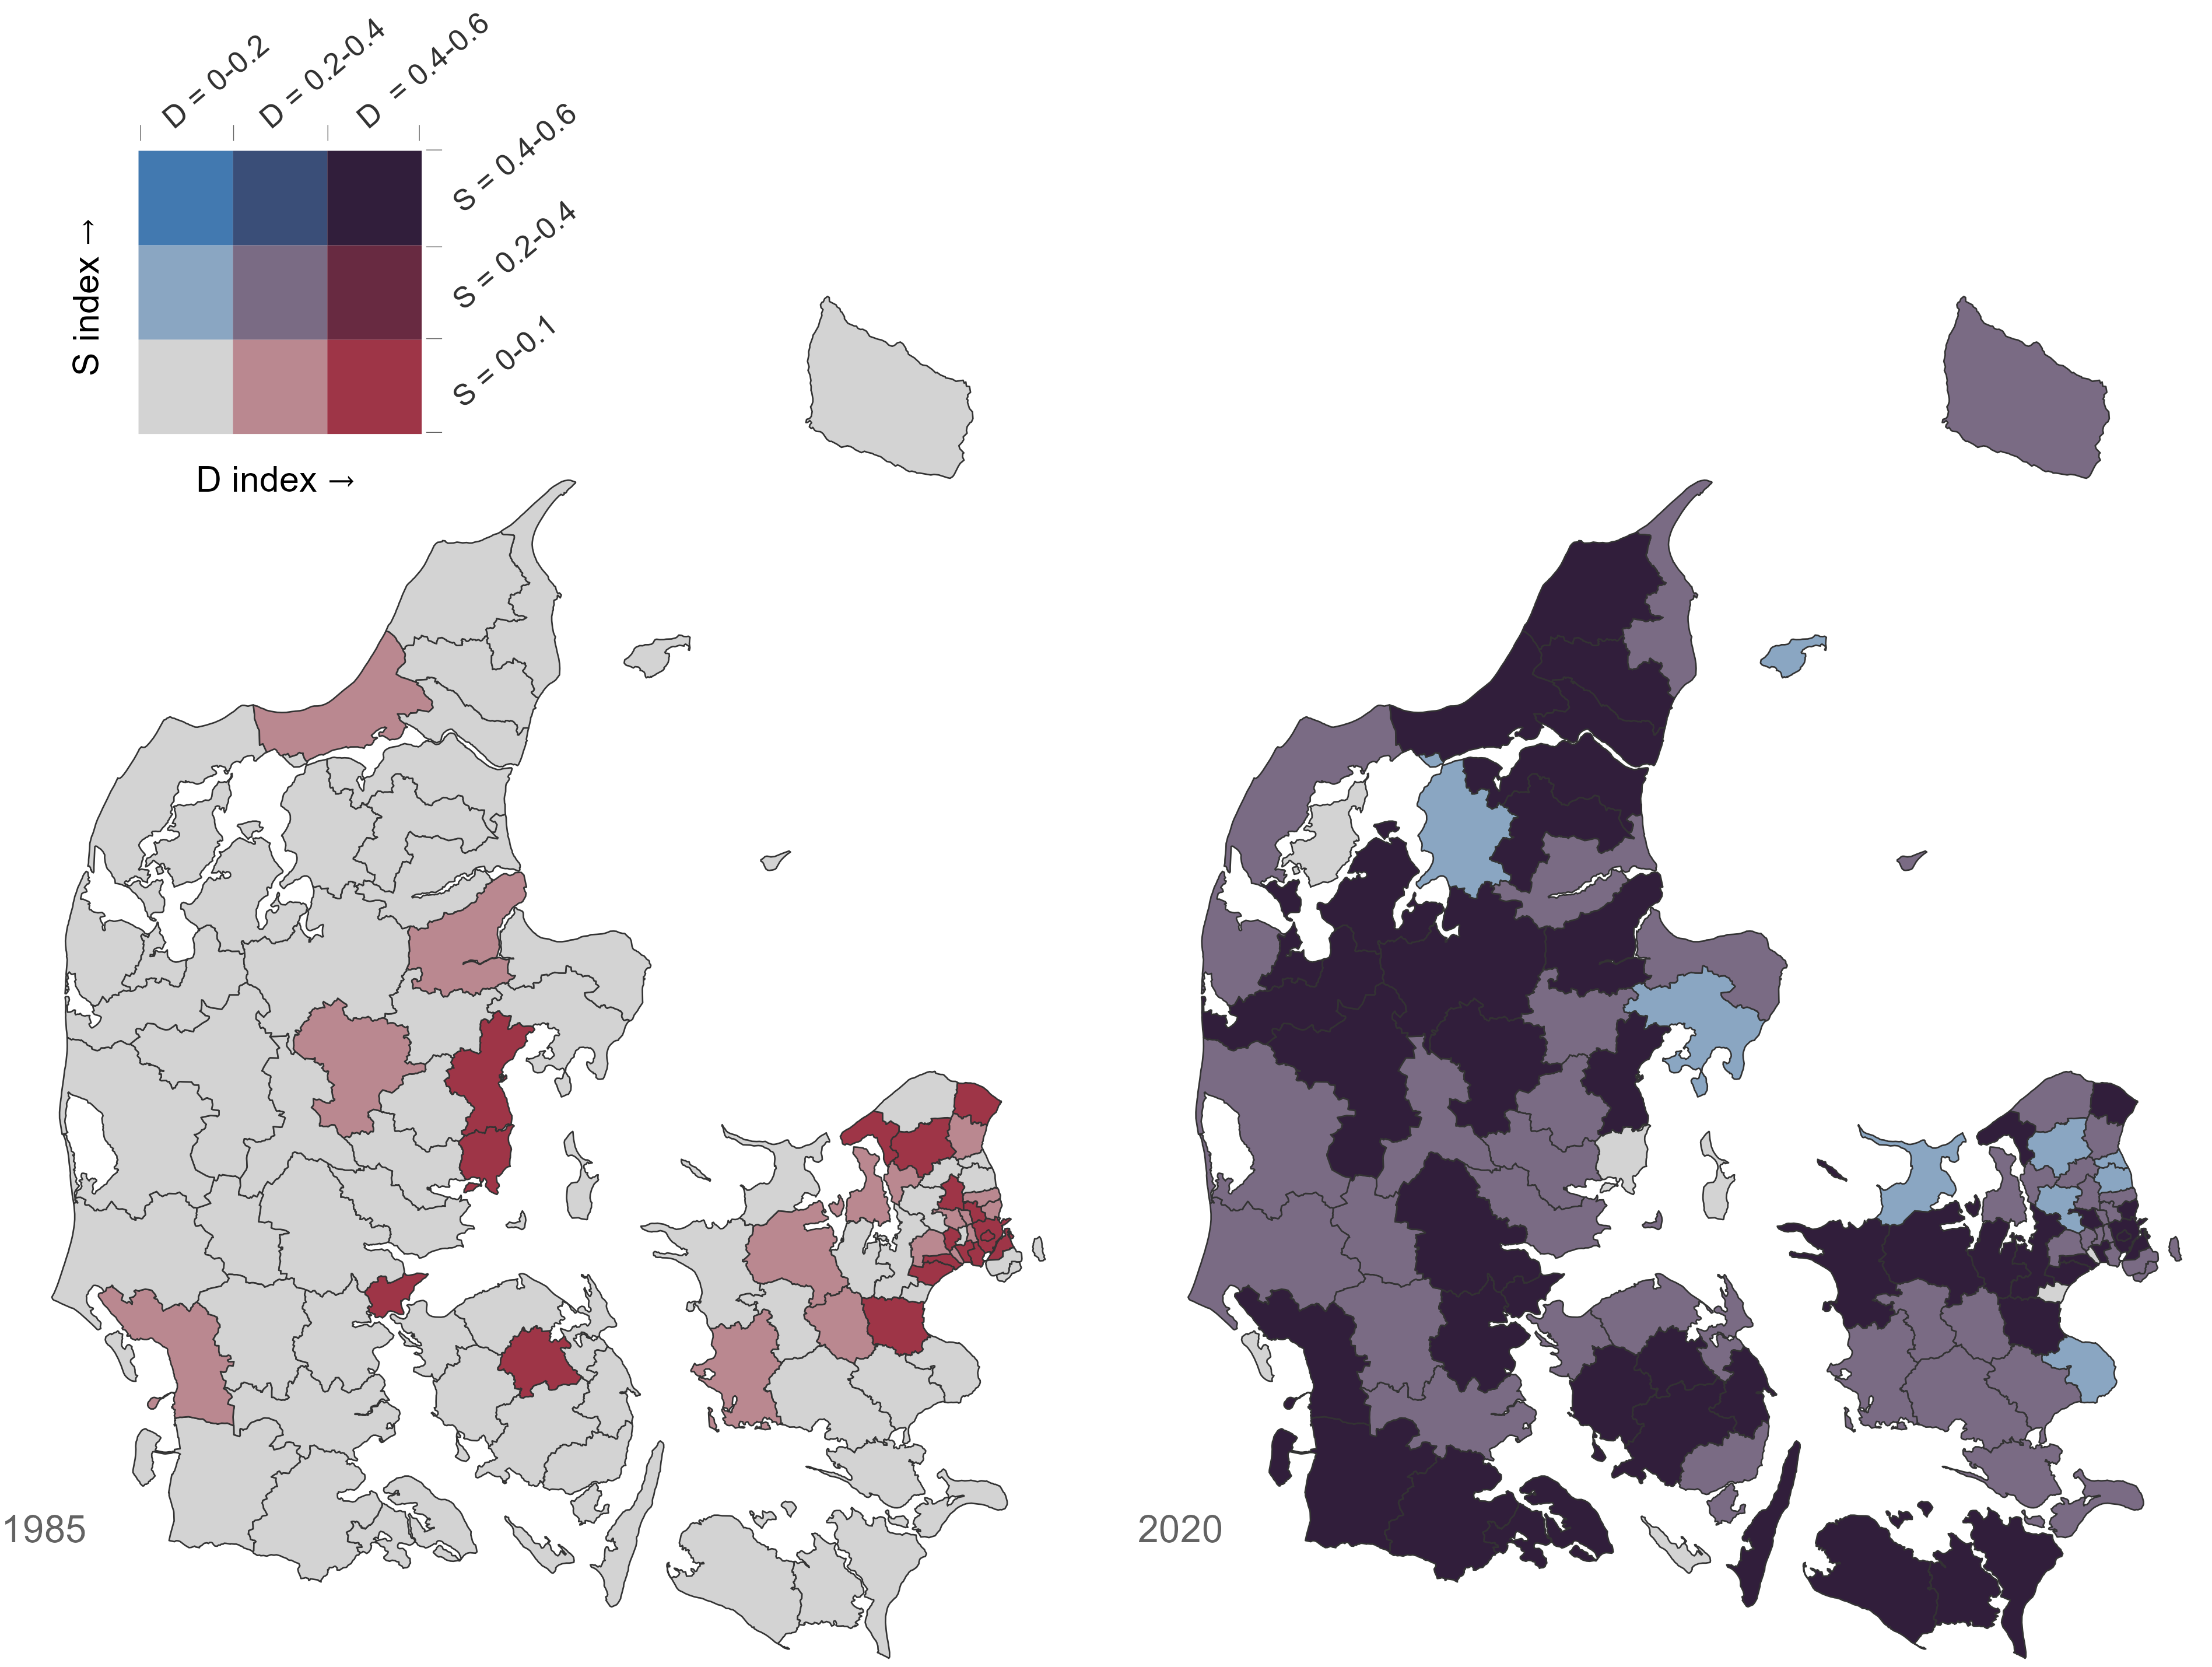
\includegraphics[width=1\linewidth]{images/Figur4} \caption{Etnisk skolesegregering i Danmark på kommunalt niveau, 1985 og 2020}\label{fig:fig-3-3}
\end{figure}

\section{Skolesegregering som produkt af boligsegregering}\label{skolesegregering-som-produkt-af-boligsegregering}

Som det blev diskuteret i \hyperref[det-danske-skolelandskab]{afsnit 1.1}, er der stor variation i koncentrationen af familier med indvandrerbaggrund og afstand mellem skoler. Som andre har vist, er koncentrationen af familier med indvandrerbaggrund ikke kun mellem kommuner, men også inden for kommuner, hvor nogle nabolag er kendetegnet ved høje koncentrationer af minoriteter---i særlig høj grad gældende for den almene boligsektor (\citeproc{ref-andersen2019a}{H. S. Andersen, 2019}; \citeproc{ref-landsbyggefonden2020}{Landsbyggefonden, 2020}). Bemærkelsesværdigt er også, at kommuner med få familier med indvandrerbaggrund angiver, at de ikke ser, at frit skolevalg fører til øget etnisk segregering, mens kommuner med mange familier med indvandrerbaggrund angiver det modsatte (\citeproc{ref-rambuxf8ll2011}{Rambøll, 2011}). Som jeg (\citeproc{ref-larsen2024c}{J. F. Larsen, 2024b}) og andre (\citeproc{ref-boterman2019}{Boterman et al., 2019}; e.g., \citeproc{ref-bunar2010}{Bunar, 2010}; \citeproc{ref-butler2007}{Butler \& Hamnett, 2007}) også har diskuteret, giver det altså en forventning om, at skolesegregering skal forstås i direkte relation til boligsegregering. Fordi de skoler, en familie enten automatisk indskrives i---distriktskolen---eller har mulighed for at vælge som alternativ, helt grundlæggende er betinget af de skoler, der er i nærheden af boligen. Dette indikerer, at mens frit skolevalg har en direkte indflydelse på graden af skolesegregering, er det ikke den primære drivkraft. Boligsegregering, hvor indvandrerfamilier bor koncentreret i bestemte områder og nabolag, spiller en større rolle i at forme de observerede grader af skolesegregering. Denne boligsegregering betyder, at fordi børn med indvandrerbaggrund ofte går i skoler i deres nærområder, hvor der er en højere koncentration af børn med samme baggrund, hvilket bidrager til skolesegregeringen. Kommuner med mange indvandrerfamilier oplever derfor større udfordringer med etnisk skolesegregering, da det frie skolevalg ofte resulterer i, at børn med dansk oprindelse vælger skoler uden for de nærområder med høj koncentration af indvandrerfamilier, hvilket yderligere forstærker segregationen.

Kigger vi på sammenhængen i segregering (\(D\)) på hhv. bolig- og skolemarkedet ser vi i Figur \ref{fig:fig-3-4}, at der er en klar sammenhæng mellem graden af bolig- og skolesegregering i de fleste kommuner, og at denne er stigende over tid (Pearson's \(r=0,50\) i 2020 mod \(r=0,29\) i 1985). Altså, de kommuner med høj boligsegregering har også typisk høj skolesegregering. Skolesegregering kan eksistere med lav boligsegregering---som Rangvid (2007) også diskuterer og viser var aktuelt frem til tidlige 2000'ere i hovedstadsområdet, og som Figur \ref{fig:fig-3-4} også illustrerer for 1985. I de seneste år ser vi en stærk sammenhæng mellem de to typer segregering i de fleste kommuner. Jeg understøtter dette yderligere med en dekomponeringsanalyse i Larsen (\citeproc{ref-larsen2024b}{2024c}). Med andre ord, selvom skolevalget principielt er ubegrænset, er der nogle skoler, der logisk er for langt væk fra hjemmet til, at hverdagen ville kunne hænge sammen. Når familier, der ligner hinanden, bor tættere på andre familier, der ligner dem selv, end de gør med familier, der er forskellige fra dem, vil der være en observerbar tendens til, at børn, som ligner hinanden, også kommer til at gå i skole sammen. Denne tendens er forstærket af at mange forældre vælger skoler baseret på, hvad de opfatter som ``god kvalitet'' og barnets trivsel, kriterier, der ofte er knyttet til skolens omdømme og dets elevgrundlag. Dette fører til, at skoler med mange ressourcestærke elever tiltrækker endnu flere af samme type, mens skoler med mange elever fra mindre ressourcestærke ikke formår at tiltrække nye familier udenfor skoledistriktet. Derfor ser vi, at segregering på boligmarkedet direkte påvirker segregeringen på skolemarkedet, hvilket skaber en selvforstærkende skolesegregerings proces.

\begin{figure}
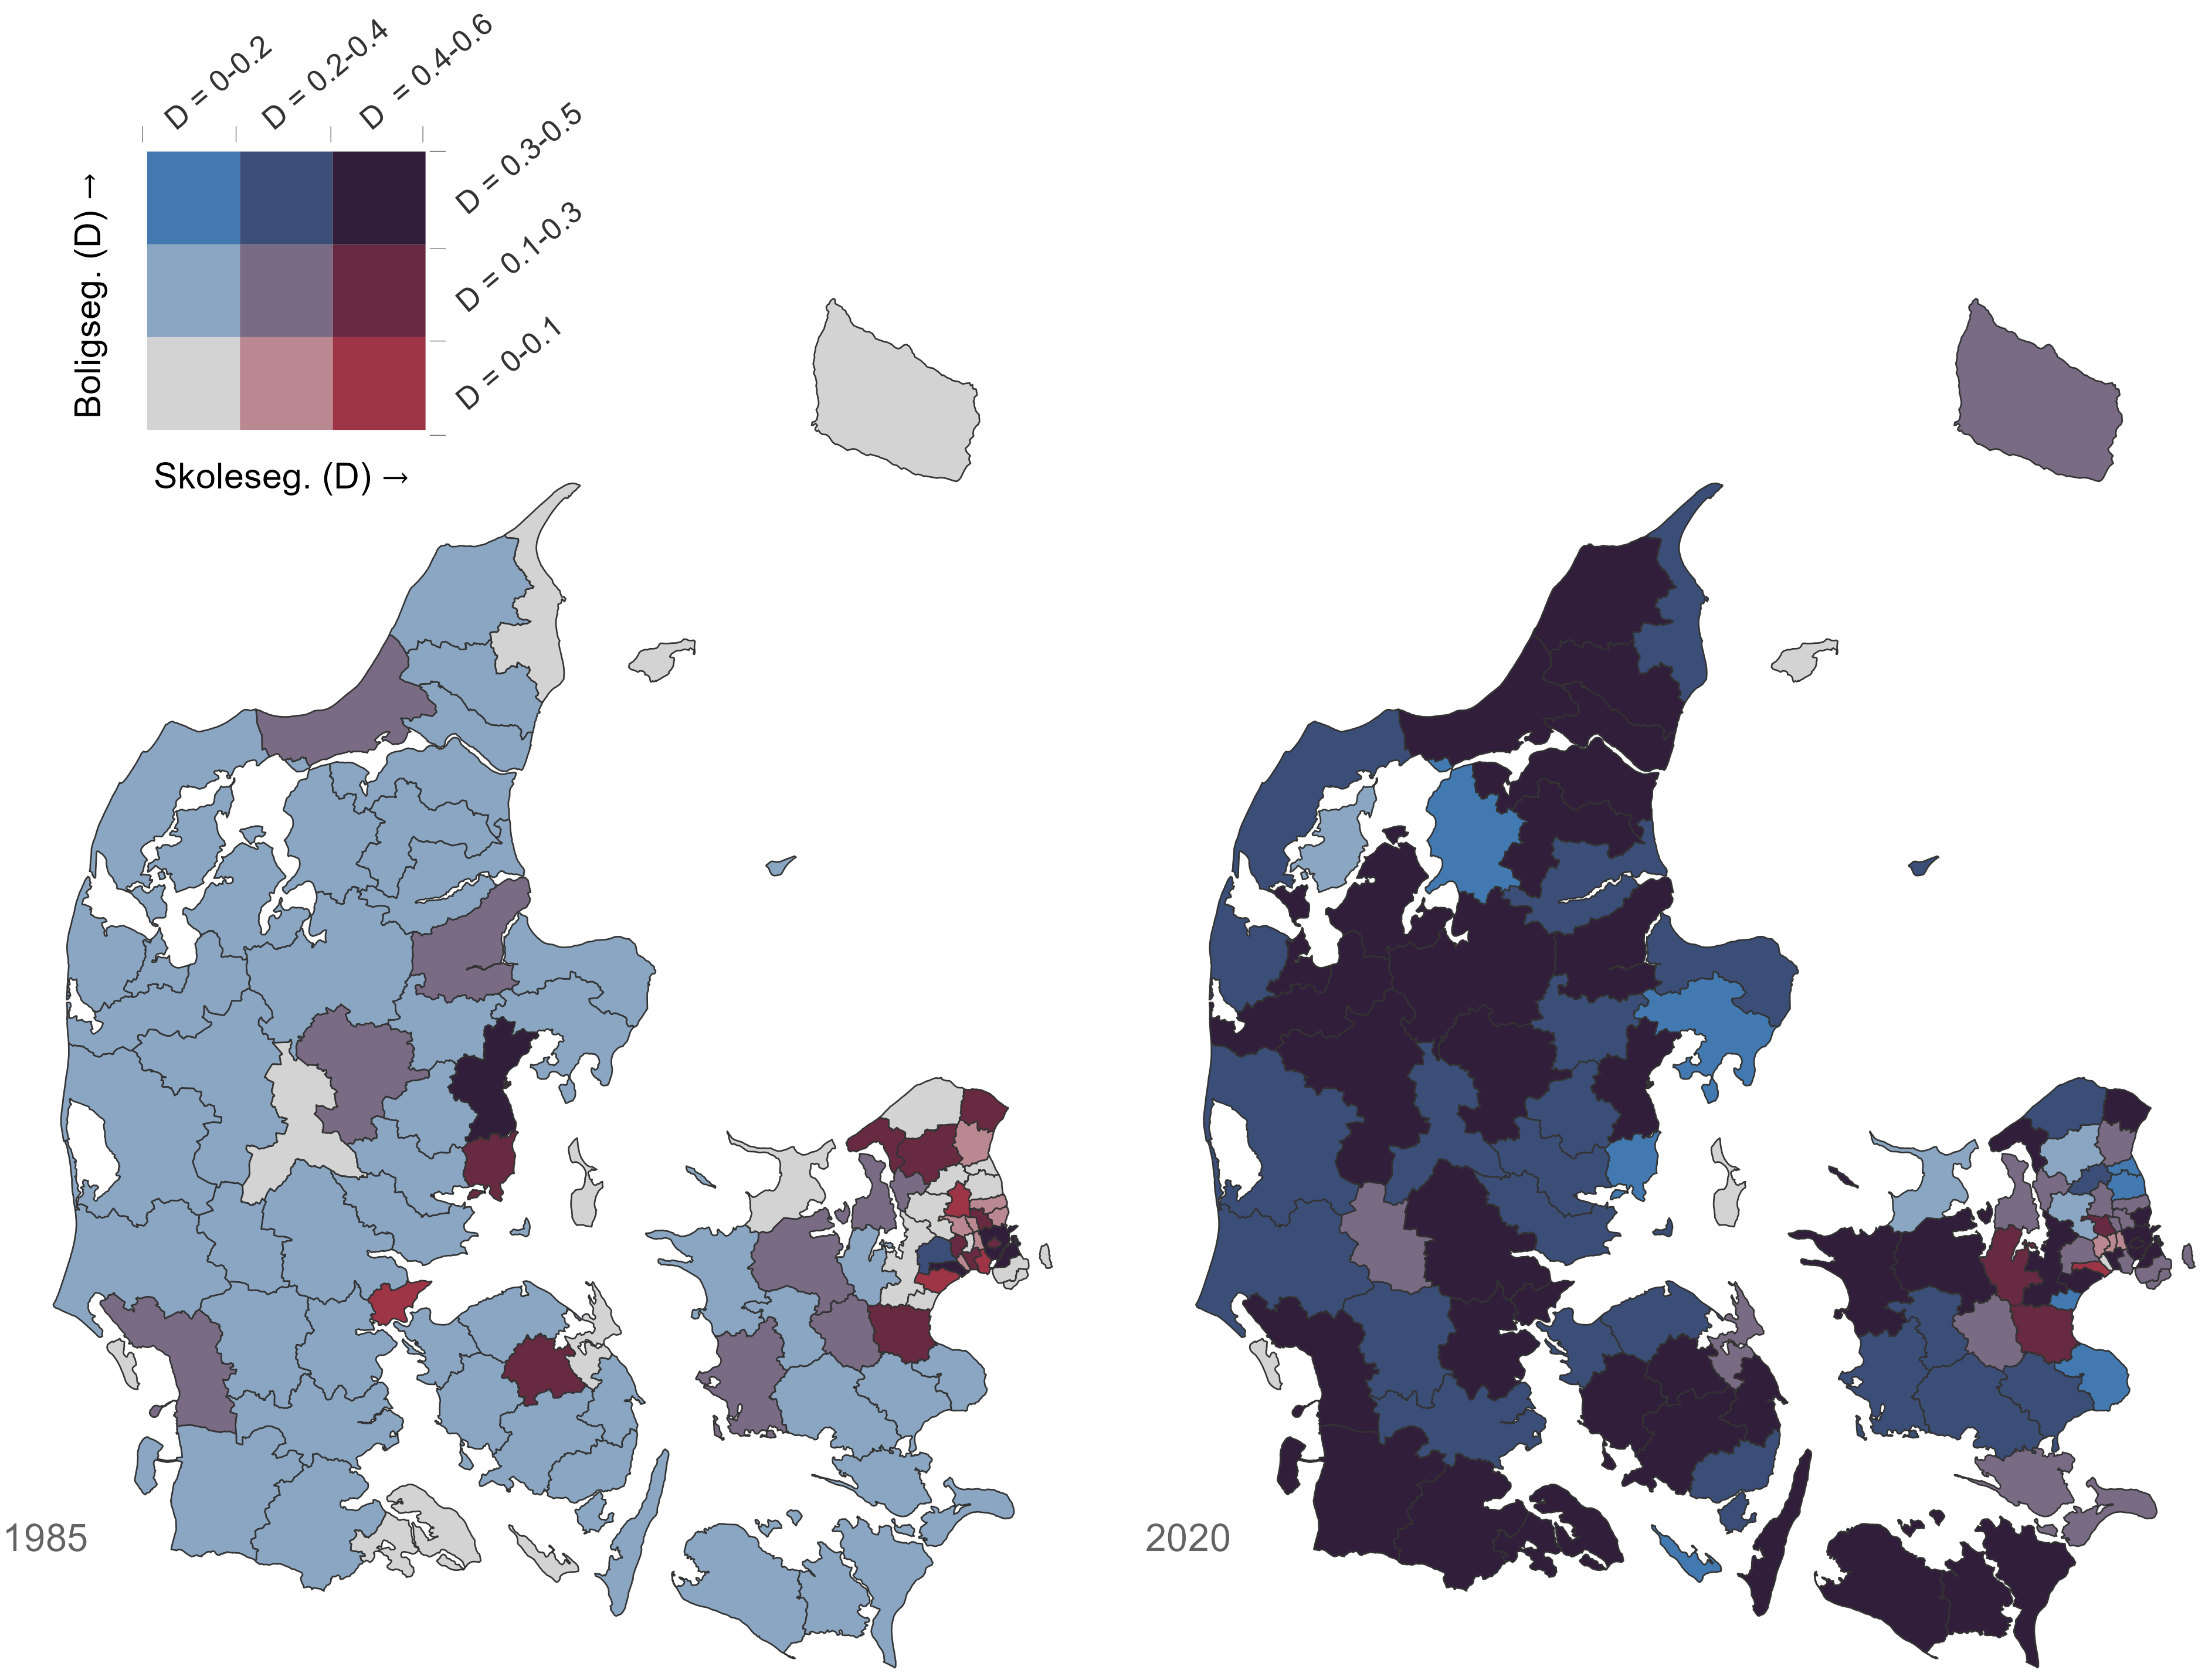
\includegraphics[width=1\linewidth]{images/Figur5} \caption{Etnisk skole- og boligsegregering i Danmark (D indeks) <br> <br> Note: *Boligsegregering er målt blandt personer, der går i den danske grundskole og ikke den fulde population. Boligsegregering er målt på sogneinddelinger og ikke skoledistrikter, da disse kun er tilgængelige for 19 kommuner og årene 2007-2017 i Danmarks Statistiks registre. Måles segregering med afsæt i skoledistrikter er sammenhængen markant mere udpræget (se @larsen2024b).*}\label{fig:fig-3-4}
\end{figure}

\newpage

\section{Konklusion}\label{konklusion}

Som bidrag til denne bogs undersøgelser og beskrivelser af mødet mellem den etnisk danske befolkning og befolkningen med indvandrerbaggrund i lyset af stigende immigration til Danmark har dette kapitel bidraget med en beskrivelse af, i hvilket omfang den danske grundskole danner et mødested for børn (og deres familier), som ikke ligner hinanden.

Som jeg har beskrevet i dette kapitel, er segregering i det danske grundskolesystem ``kun'' moderat---og segregering har på nogle parametre været faldende over tid på grund af ændrede strukturelle forhold, såsom en større minoritetsbefolkning i de fleste kommuner. Det vil sige, at de danske skoler er mødesteder på tværs af etniske gruppeskel---men omfanget af møder i denne arena er langt fra ``optimalt udnyttet'', og den positive udvikling har været langsom. Samtidig er der tendenser, der tegner et ikke-optimistisk billede af udviklingen. Den langsomme udvikling af mere blandede skoler skal tilskrives den disproportionalt geografiske koncentration af familier med indvandrerbaggrund i bestemte kommuner og nabolag. Dette betyder, at selvom der er potentiale for mere integration i skolerne, begrænses dette i høj grad af, hvor folk bor.

Grunden til at vi interessere os for skolesegregering er selvfølgelig ikke det tekniske oprids af hvorfor segregering kan opstå. Vi er interesseret fordi der er en grundlæggende tro på at det betyder noget for vores samfund, som diskuteret indledningsvist i dette kapitel og i \hyperref[kap1]{kapitel 1}. Børn med dansk oprindelse er blevet mere eksponeret til børn med indvandererbaggrund i en skolekontekst. Fra \(7\%\) i 1985 til \(19\%\) i 2020. Der er altså forventeligt flere sociale relationer på tværs af etniske gruppeskel i de formative år. På den anden side er eksponeringen til andre børn med indvandererbaggrund blandt børn der selv har indvandererbaggrund steget fra \(16\%\) til \(35\%\). Det vil sige at i takt med stigende indvandring og ændrede demografiske forhold i populationen, bliver dele af minoritetsgruppe forholdsvis mere ''isoleret'' i skolelandskabet, grundet en kombination af bosætningsmønstre og tendenser i hvem der udnytter skolevalget.

Så selvom udviklingen ikke er så ekstrem som dele af den offentlige debat anleder til at tro, affejer resultaterne dog ikke en grundlæggende bekymring på lokale niveauer. Mit centrale budskab er, at problemets omfang ikke har rod i eksistensen af frit skolevalg, som andre også argumenterer for (f.eks. Rambøll (\citeproc{ref-rambuxf8ll2011}{2011}) eller Gandil i Zetland (\citeproc{ref-zetland2018}{2018})). Ikke at skolevalget ingen betydning har, men skolevalg øger kun segregering i bestemte områder over det strukturelt bestemte niveau (\citeproc{ref-rangvid2010}{Rangvid, 2010}); skolevalget er ikke den mekanisme, der skaber segregering. I stedet skal skolesegregering forstås først og fremmest som et produkt af bosætningsmønstre, da disse har en fundamental betydning for, hvilke skoler der er tilgængelige for den enkelte familie, uafhængigt af familiens muligheder for at vælge alternativer til distriktskolen. Hvad der yderligere bidrager til skolesegregering er, at disse muligheder samtidig er betinget af, at de alternative skoler rent faktisk har plads til flere elever---hvilket de mest populære skoler sjældent har (\citeproc{ref-rambuxf8ll2011}{Rambøll, 2011}). Dette betyder, at selvom frit skolevalg kan forstærke eksisterende segregeringsmønstre, er det ikke den primære drivkraft bag segregering. For at tackle skolesegregering effektivt, skal vi fokusere på at adressere de underliggende bosætningsmønstre og sikre, at der er tilstrækkelige og attraktive skolemuligheder til rådighed for alle familier, uanset hvor de bor.

\chapter{Arbejdspladser som mødested}\label{kap5}

\emph{\href{https://vbn.aau.dk/en/persons/albrekt}{Christian Albrekt Larsen}}, \href{https://vbn.aau.dk/en/persons/led}{Laciné E. N. Diop} og \emph{\href{https://vbn.aau.dk/da/persons/jeppefl}{Jeppe Fjeldgaard Larsen}}


\includegraphics[width=1\linewidth]{images/dalle-work}

Indvandrernes og efterkommerens succes, eller manglende succes, på arbejdsmarkedet har været centralt i både politiske og akademiske diskussioner. Med god ret, da økonomiske ressourcer er centralt for at skabe gode liv for indvandrere og deres efterkommere. Men ansigt-til-ansigt interaktionen på arbejdspladserne er også centralt for at opbygge sociale relationer og nedbryde eventuelle fordomme på tværs af etniske skel, se \hyperref[kap1]{kapitel 1} og \hyperref[kap6]{kapitel 6}. Arbejdspladserne har således ikke bare potentiel til at forandre indvandrere og efterkommere. De har også potentiale til at forandre majoriteten.

Arbejdspladser er en mødeplads, hvor majoritet og minoriteter interagerer intensivt med hinanden, jævnfør \hyperref[kap1]{kapitel 1}, selvom man ikke bor sammen eller har børn der går i skole sammen. En række studier har fundet sammenhæng mellem den etniske komposition af arbejdssteder og sociale relationer og fravær af etniske fordomme (\citeproc{ref-andersson2021}{Andersson \& Dehdari, 2021}; \citeproc{ref-thomsen2012}{Frølund Thomsen, 2012}; \citeproc{ref-kokkonen2015}{Kokkonen et al., 2015}; \citeproc{ref-mancini2018}{Mancini et al., 2018}; \citeproc{ref-mutz2006}{Mutz \& Mondak, 2006}; \citeproc{ref-pagotto2010}{Pagotto et al., 2010}; \citeproc{ref-rydgren2013}{Rydgren et al., 2013}; \citeproc{ref-vassou2017}{Vassou et al., 2017}).

I dette kapitel beskrives, hvor meget majoritet og minoritet er eksponeret overfor hinanden på arbejdspladsen. Kapitlet er opdelt i fem afsnit. I den første afsnit beskriver vi hvordan vi har regnet på arbejdspladsen som et mødested. Dernæst beskriver vi resultaterne for majoritetens eksportering til indvandrere/efterkommere. Afsnit to beskriver den gennemsnitlige eksponering, mens afsnit tre beskriver andel af majoriteten, der ikke eksponeres for én eneste indvandrere/efterkommer på deres arbejdsplads. Afsnit tre og fire laver samme beskrivelse, set fra minoritetens synsvinkel. Endeligt opsummeres kort i det sidste afsnit.

\section{Den etniske sammensætning af arbejdspladser}\label{den-etniske-sammensuxe6tning-af-arbejdspladser}

Den etniske sammensætning af arbejdspladser er ret ubeskrevet både nationalt og internationalt. Men de opgørelser der findes, hæfter sig normalt ved en stærk etnisk opdeling af arbejdsmarkedet. I den amerikanske assimileringslitteratur har man ikke haft datamaterialet til at lave detaljerede beskrivelser af den etniske komposition af arbejdspladser.\footnote{Men i forlængelse af borgerrettighedsbevægelsen i 1960erne blev alle arbejdspladser med \(100\) ansatte og derover dog forpligtet til at indrapportere den racemæssige komposition af amerikanske arbejdspladser. Disse data viser, at afroamerikanernes større succes på det amerikanske arbejdsmarked \emph{ikke} omsætter sig til mere racemæssig diversitet på arbejdspladsen. Tværtimod har segregering været stigende på tværs af racer i USA (OBS OBS OBS Hellerstein, Judith et al, 2008; Hellerstein, Judith K. \& Neumark, 2008 OBS OBS OBS)} I en europæisk kontekst viser et svensk studie, at majoritetsbefolkningen og indvandrere og efterkommere i perioden fra 1985 til 2001 blev mere ulige fordelt på arbejdspladser; målt som større sandsynlighed for at være eksponeret for sin egen gruppe på arbejdspladsen. Det gælder efter, at man har taget højde for forandringer i gruppestørrelse og en række andre forhold (\citeproc{ref-uxe5slund2010}{Åslund \& Skans, 2010}). Et tysk studie viser ligeledes, at den etniske sammensætning af arbejdspladser er meget skæv, men dog blev en smule bedre i perioden fra 1980 til 2008 (\citeproc{ref-glitz2014}{Glitz, 2014}).

Diop-Christensen \& Larsen (\citeproc{ref-diopchristensen2024}{2024}) har lavet et nyligt studie af sammensætningen i Danmark, hvilket er udgangspunkt for dette kapitel. De danske registrer gør det muligt at sammenkøre data om personers herkomst, se \hyperref[kap3]{kapitel 3}, med \href{https://www.dst.dk/Site/Dst/SingleFiles/GetArchiveFile.aspx?fi=659482655935&fo=0&ext=kvaldel}{Danmark Statistisks klassifikation} af såkaldte arbejdssteder. Sidstnævnte er produktionsenheder, der er afgrænset til én fysisk adresse. Det er vigtigt da store virksomheder som f.eks. Arla og Novo Nordisk har mange arbejdssteder i og udenfor Danmark. Diop-Christensen \& Larsen (\citeproc{ref-diopchristensen2024}{2024}) starter opgørelsen i 1996, da det er det første år, hvor Danmarks Statistik har opgjort den type af job, som en person er beskæftiget i (\href{https://www.dst.dk/Site/Dst/SingleFiles/GetArchiveFile.aspx?fi=2299282738&fo=0&ext=kvaldel}{DISKO-klassifikation}). Det er vigtigt, da man godt kan forestille sig arbejdspladser, hvor indvandrere og efterkommere varetager funktioner, som majoriteten ikke varetager.

Diop-Christensen \& Larsen (\citeproc{ref-diopchristensen2024}{2024}) finder, at det danske arbejdsmarked i perioden fra 1996 til 2019 er blevet mere segregeret; målt med et såkaldt justeret Dissimilarity Index (D) (se \hyperref[kap4]{kapitel 4} eller \hyperref[bilagA]{Bilag A}). Deres estimat er, at segregeringen blev målt som \(D=0,21\) i 1996. Tolkningen af dette er, at i 1996 skulle man flytte \(21\%\) af alle beskæftigede indvandrere/efterkommere, eller \(21\%\) af alle beskæftigede med dansk-dansk herkomst (se \hyperref[kap3]{kapitel 3}) til en arbejdsplads med hhv. lavere eller højere andel beskæftigede med indvandrerbaggrund for at få en fordeling, der matcher resultatet fra en tilfældig fordeling af de to grupper på alle danske arbejdspladser. I 2019 er den andel vokset til \(33\%\) (\(D=0,33\)). I tråd med andre analyser indikerer resultatet en stigende etniske segmentering af det danske arbejdsmarked.

Koncentration af indvandrere, typisk i de manuelle jobs, betyder imidlertid ikke, at arbejdspladser er blevet mindre relevante for mødet mellem majoriteten og etniske minoriteter. Tværtimod viser Diop-Christensen \& Larsen (\citeproc{ref-diopchristensen2024}{2024}), at samtidigt med, at arbejdsmarkedet segregeres, så stiger sandsynligheden for, at majoriteten arbejder på en arbejdsplads med indvandrere og efterkommere.

Figur \ref{fig:fig-5-1} illustrerer, Diop-Christensen \& Larsen (\citeproc{ref-diopchristensen2024}{2024}) beregner arbejdsstedseksponeringen for de beskæftigede. Målet for eksponering kan variere mellem \(0\), hvor ingen andre på arbejdspladsen tilhører den ''anden'' gruppe (majoritet/minoriteter), og \(100\%\), hvor alle andre på arbejdspladsen tilhører den ''anden'' gruppe (majoritet/minoriteter).

\begin{figure}
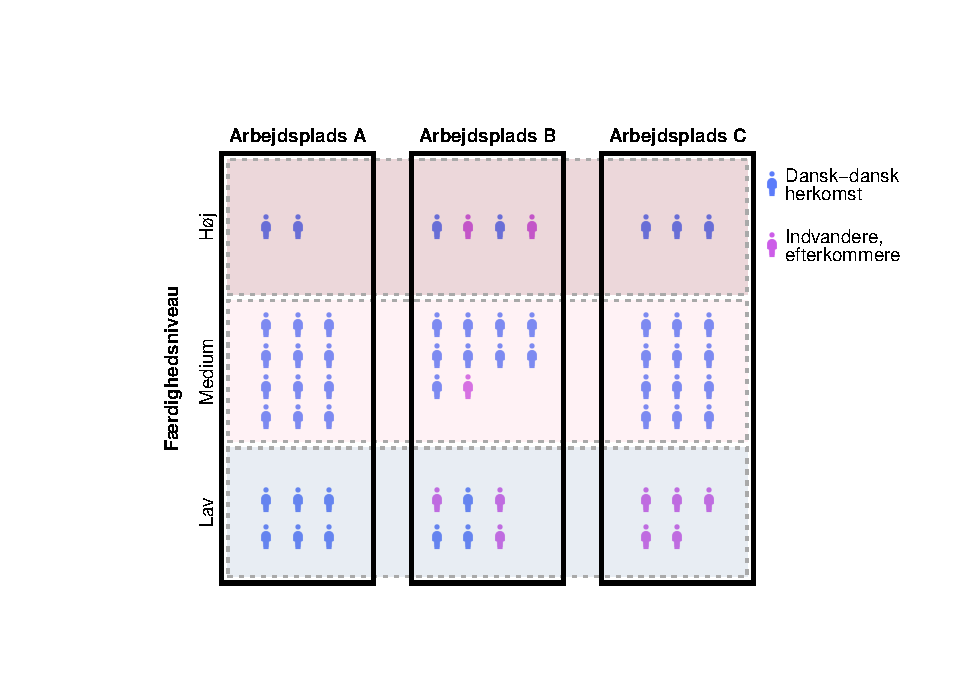
\includegraphics[width=1\linewidth]{en-befolkning-blander-sig_files/figure-latex/fig-5-1-1} \caption{Illustration af eksponering på arbejdspladsen.}\label{fig:fig-5-1}
\end{figure}

Arbejdsplads \textbf{A} i Figur \ref{fig:fig-5-1} er en illustration på, hvordan de \(20\) beskæftigede med dansk-dansk herkomst ikke er eksponeret for én eneste indvandrer eller efterkommer på deres arbejdsplads, dvs. eksponeringen er \(0\).

På arbejdsplads \textbf{B} i Figur \ref{fig:fig-5-1} er seks af de ansatte indvandrere eller efterkommere. Dermed er en person med dansk-dansk herkomst eksponeret til \(6\) personer fra ''den anden'' grupper. Det svarer til \(32\%\), hvilket vi betegner graden af eksponering.\footnote{I eksemplet er gruppen med dansk-dansk herkomst eksponeret til \(13\) fra egen gruppe ---det samlede antal minus personen selv---eller \(\approx 74\%\), hvilket kan betegnes som grade af isolation kaldet \emph{isolation}, Bell (\citeproc{ref-bell1954}{1954}), se \hyperref[bilagA]{Bilag A}).} Omvendt er en indvandrer/efterkommer eksponeret til \(14\) med dansk-dansk herkomst og \(5\) fra sin indgruppe, svarende til en eksponering på \(\approx 74\%\).

Eksponering kan således tolkes som sandsynligheden for, at den næste man interagerer med på arbejdspladsen, er en fra den modsatte gruppe. Arbejdsplads \textbf{B} er et eksempel på det typiske forhold, at indvandrere og efterkommere har større sandsynlighed for at blive eksponeret for den modsatte gruppe end det er tilfælde for majoritetsgruppen.

Arbejdsplads \textbf{C} i Figur \ref{fig:fig-5-1} er en illustration på en situation, hvor arbejdspladsen er meget internt opdelt mellem stillinger, der har forskelligt færdighedsniveauer. Her arbejder de fem medarbejdere med indvandrerbaggrund i det Diop-Christensen \& Larsen (\citeproc{ref-diopchristensen2024}{2024}) benævner lavt færdighedsniveau.\footnote{DISKO-klassifikation 9, i Danmarks Statistiks registrer.} Det er typisk ufaglærte jobs, som for eksempel rengøringsarbejde eller andet manuelt arbejde i primære erhverv. På arbejdsplads \textbf{C} er dem med dansk-dansk herkomst i højere interne stillinger, hvilket formentligt gør samarbejdet på tværs af etniske skel mindre sandsynligt og mindre intensivt. Derfor supplerer Diop-Christensen \& Larsen (\citeproc{ref-diopchristensen2024}{2024}) de generelle eksponeringsmål med et *beskæftigelsesspecifik-eksponeringsmål.\footnote{Det vil sige eksponeringen indenfor faglighedsniveauer på de enkelte arbejdspladser. På arbejdsplads \textbf{C} vil det mål være \(0\) for begge grupper, da hverken dem med dansk-dansk herkomst eller indvandrerne/efterkommerne er eksponeret for den anden gruppe i den samme beskæftigelsesgruppe. På Arbejdsplads \textbf{B} derimod, er indvandrere/efterkommere i stillinger med lavt faglighedsniveau eksponeret for \(3\) fra majoriteten og to andre minoriteter, hvilket giver en beskæftigelsesspecifik eksponering på \(60\%\), hvilket er \emph{lavere} end eksponering udregnet på baggrund af hele arbejdsstedet (\(74\%\)). En beskæftiget med dansk-dansk herkomst i en stilling med lavt faglighedsniveau på arbejdsplads \textbf{B} har ligeledes en beskæftigelsesspecifik eksponering på \(60\%\), hvilket er \emph{højere} end eksponeringsgraden udregnet på baggrund af hele arbejdsstedet (\(32\%\)). Diop \& Larsen (2024) viser, at den generelle og beskæftigelsesspecifikke eksponering varierer for det begrænsede antal i stillinger med lavt faglighedsniveau, typisk ufaglærte jobs, mens forskellene er ubetydelige for det samlede arbejdsmarkedet. Derfor anvender vi i det kapitel primært det simple mål for eksponering på arbejdspladsen.}

\section{Gennemsnitlig eksponering til indvandrere og efterkommere på arbejdspladser}\label{gennemsnitlig-eksponering-til-indvandrere-og-efterkommere-puxe5-arbejdspladser}

Det stigende antal indvandrere og efterkommere på arbejdsmarkedet fra 1996 til 2019 har bevirket, at størstedelen af beskæftigede med dansk-dansk herkomst er kommet til at arbejde sammen med indvandrere og efterkommere. Der er selvfølgelig stor variation i eksponeringen. Nogle er ikke eksponeret til én eneste indvandrer eller efterkommer på arbejdspladsen, se nedenstående beskrivelse af graden af ''isolation'', mens andre er eksponeret for mange.

Majoritetens gennemsnitlige eksponering til indvandrere og efterkommere på arbejdspladsen giver en god fornemmelse af udviklingen over tid. Diop \& Larsen estimerer, at majoritetens gennemsnitlig eksponering er steget fra \(3,1\%\) i 1996 til \(13,3\%\) i 2019.

I Figur \ref{fig:fig-5-2} er den gennemsnitlig eksponering opdelt på kommunalt niveau. I 1996, kortet placeret til venstre i 5.2, var til kun i hovedstadsområdet, Aarhus og enkelte grænselandskommuner, at det var typisk at være eksponeret til 3 -- 7 procent indvandrere/efterkommere på arbejdspladsen (markeret med blåt). I 2019, kortet placeret il højre i figur 5.2, ser situationen helt anderledes ud. I alle kommuner er det nu normalen, at majoriteten er eksponeret til 3 -- 7 procent indvandrere/efterkommere på deres arbejdsplads. I store del af landet ligger den gennemsnitlige eksponering nu over 7 procenter, markeret med gullige/grønlige farver.

\begin{figure}
\includegraphics[width=1\linewidth]{images/Figur_4_1} \caption{Beskæftigedes med dansk-dansk herkomst gennemsnitlige eksponering til indvandrere/efterkommere på deres arbejdspladsen i 1996 (venstre) og 2019 (højre). <br> <br> **Note**: *Opgjort på tværs af kommuner.*}\label{fig:fig-5-2}
\end{figure}

Dette billede af stigende eksponering af de beskæftigede med dansk-dansk herkomst kan nuanceres på mange forskellige måder. For gruppen af majoriteten beskæftiget i stillinger med lavt færdighedsniveau er den gennemsnitlige eksponering cirka to procentpoint højere i 2019, når der måles på beskæftigelsesspecifik eksponering, frem for generel eksponering. Det gør således en forskel, hvordan man måler, men det rykker ikke ved det overordnet billede.

Mere interessant er det måske, hvor meget majoriteten på deres arbejdsplads der blevet eksponeret til indvandrere og efterkommere med muslimsk baggrund. Diop-Christensen \& Larsen (\citeproc{ref-diopchristensen2024}{2024}) estimerer, at de beskæftigede med dansk-dansk herkomst (gennemsnitlige) eksponering til MENAPT-indvandrere/efterkommere på arbejdspladsen i 1996 var \(0,6\%\). Den (gennemsnitlige) eksponering er i 2019 steget til \(2,5\%\). Den mindre eksponering til muslimske minoriteter skyldes primært, at der er tale om en mindre gruppe, men det skyldes også en koncentration af muslimske minoriteter i de store bykommuner, hvilket illustreres i Figur \ref{fig:fig-5-3}.

I 1996, det venstre kort Figur \ref{fig:fig-5-3}, var det kun på Sjælland, i Odense og Aarhus, at det var typisk, at majoriteten var eksponeret til en til to procent indvandrere/efterkommere fra MENAPT-lande på deres arbejdsplads. Markeret med blå farver. I 2019, det højre kort, er det nu typisk i hele landet at have et sådant eksponeringsniveau til muslimske minoriteter, med undtagelse af Lemvig kommune. Men det stadigt tydeligt, at eksponering til minoriteter fra muslimske oprindelseslande er højst omkring hovedstadsregionen, Odense og Aarhus, se gullige og grønlige farver i Figur \ref{fig:fig-5-3}.

\begin{figure}
\includegraphics[width=1\linewidth]{images/Figur_4_2} \caption{Andelen af beskæftigede med dansk-dansk herkomst, der ikke er eksponeret til én eneste indvandrer eller efterkommer på deres arbejdsplads i 1996 (venstre) og 2019 (højre). <br> <br> **Note**: *Opgjort på tværs af kommuner. *}\label{fig:fig-5-3}
\end{figure}

\section{Majoritetens ''isolation'' fra minoriteterne}\label{majoritetens-isolation-fra-minoriteterne}

En anden måde at opgøre det på, er at se på andelen af beskæftigede med dansk-dansk herkomst, der ikke har én eneste indvandrere eller efterkommere på deres arbejdsplads. En sådan ''isolation'' er selvfølgelig langt mere sandsynlig på små end på store arbejdspladser. Ikke desto mindre giver andelen med \emph{nul-eksponering} også en god fornemmelse af forandringer over tid. Diop-Christensen \& Larsen (\citeproc{ref-diopchristensen2024}{2024}) estimerer, at andelen af beskæftigede med dansk-dansk herkomst, som er ''isolerede'' på deres arbejdsplads er faldet fra \(45\%\) i 1996 til \(29\%\) i 2019.

\begin{figure}
\includegraphics[width=1\linewidth]{images/Figur_4_3} \caption{Beskæftigedes med dansk-dansk herkomst gennemsnitlige eksponering til MENAPT indvandrere/efterkommer på deres arbejdsplads i 1996 (venstre) og 2019 (højre). <br> <br> **Note**: *Opgjort på tværs af kommuner. MENAPT dækker over ...*}\label{fig:fig-5-4}
\end{figure}

I Figur \ref{fig:fig-5-4} er ''isolationen'' opdelt på tværs af kommunerne. Andelen med \emph{nul-eksponering} er faldet i stort set hele landet. I 1996, det venstre kort i Figur \ref{fig:fig-5-4}, var situationen i største parten af landet, at \(43\) procent eller flere, af de beskæftigede fra majoriteten, i en given kommune, ikke arbejdede sammen med en eneste indvandrer eller efterkommer. Det er markeret med gullige og grønlige farver i figuren. I 2019 ser situationen helt anderledes ud. I størsteparten af landet er det nu atypisk at have så mange ''isolerede'' i en kommune, se Figur \ref{fig:fig-5-4}.

\section{Minoriteters eksponering til majoritetsbefolkningen}\label{minoriteters-eksponering-til-majoritetsbefolkningen}

Beskæftigede indvandrere og efterkommere er i høj grad eksponeret til beskæftigede med dansk-dansk herkomst på deres arbejdsplads. Diop-Christensen \& Larsen (\citeproc{ref-diopchristensen2024}{2024}) estimerer, at den gennemsnitlige eksponering var \(74\%\) i 1996. Opdelt på kommuner viser den venstre del af Figur \ref{fig:fig-5-5}, at den (gennemsnitlige) høje eksponering til majoritetsbefolkningen i 1996 gjorde sig gældende i hele landet. Med undtagelse af et par enkelte kommuner i hovedstadsområdet var den gennemsnitlige eksponering på \(67\) procent eller derover. Det er markeret med grønlige og gullige farver i Figur \ref{fig:fig-5-5}.

\begin{figure}
\includegraphics[width=1\linewidth]{images/Figur_4_4} \caption{Beskæftigede indvandreres/efterkommeres gennemsnitlige eksponering til beskæftigede med dansk-dansk herkomst på deres arbejdsplads i 1996 (venstre) og 2019 (højre). <br> <br> **Note**: *Opgjort på tværs af kommuner.*}\label{fig:fig-5-5}
\end{figure}

Efterhånden som der kommer flere og flere indvandrere og efterkommere ind på arbejdspladserne, så falder den gennemsnitlige eksponering til beskæftigede med dansk-dansk herkomst. Diop-Christensen \& Larsen (\citeproc{ref-diopchristensen2024}{2024}) estimerer, at den (gennemsnitlige) eksponering i 2019 er \(57\%\). I den nederste del af Figur \ref{fig:fig-5-5} ses den eksponeringen på tværs af beskæftigede bosat i forskellige kommuner. Den lysere farve indikerer, at eksponeringen falder. Det er dog værd at bemærke, at eksponeringen til kolleger med dansk-dansk herkomst stadig er højere end eksponeringen til indvandrere og efterkommere på arbejdspladsen. Det typiske er således fortsat, at indvandrere og efterkommere har større sandsynlighed for at arbejde sammen med en fra majoriteten end en med minoritetsbaggrund.

\section{Minoriteters ''isolation'' fra majoritetsbefolkningen}\label{minoriteters-isolation-fra-majoritetsbefolkningen}

Ligesom for majoriteten, beregner Diop-Christensen \& Larsen (\citeproc{ref-diopchristensen2024}{2024}) også andelen af beskæftigede indvandrere og efterkommere, der ikke er eksponeret til én eneste med dansk-dansk herkomst. Andelen af minoriteter i ''isolation'' er markant mindre end det er tilfældet for majoriteten. Studiet estimerer andelen af ''isolerede'' indvandrere/efterkommere til at være \(13\%\) i 1996 og \(14\%\) i 2019. Fra 1996 til 2019 er der således stort set ikke sket nogen stigning i andelen af indvandrere/efterkommere, der arbejder på en arbejdsplads, der ikke minimum er én ansat fra majoriteten.

I Figur \ref{fig:fig-5-6} vises andelen af ''isolerede'' på tværs af kommuner i 1996 (venstre) og 2019 (højre). I 1996, det venstre kort, var der ikke noget klart mønster i, hvor der \(18\) procent eller flere ''isolerede''; markeret med grøn og gullige farver. I 2019, det højre kort, viser det sig, en højre andel ''isolerede'' udelukkende forekommer på Sjælland og Fyn, men det er ikke et klart mønster.\footnote{Beregninger på Løsø kommune er meget usikre pga. et meget begrænset antal indvandrere/efterkommere.}

\begin{figure}
\includegraphics[width=1\linewidth]{images/Figur_4_5} \caption{Andelen af beskæftigede indvandrere/efterkommere der ikke er eksponeret til én eneste med dansk-dansk herkomst på deres arbejdsplads i 1996 (venstre) og 2019 (højre). <br> <br> **Note**: *Opgjort på tværs af kommuner.*}\label{fig:fig-5-6}
\end{figure}

For indvandrere og efterkommere ansat i stillinger, der kræver lavt færdighedsniveau, er eksponeringen til gruppen med dansk-dansk herkomst mindre. Diop-Christensen \& Larsen (\citeproc{ref-diopchristensen2024}{2024}) estimerer, at gruppen beskæftigelsesspecifikke eksponering i 2019 er på \(37\%\), hvilket er markant mindre end for den samlede gruppe af indvandrere og efterkommere. Endeligt er gruppen fra MENAPT-lande generelt en smule mindre eksponeret til kolleger med dansk-dansk-herkomst end indvandrere og efterkommere generelt. I 1996 var den gennemsnitlige eksponering \(60\%\), hvilket i 2019 var faldet til \(55\%\).\footnote{Andelen af beskæftigede MENAPT-indvandrere/efterkommere, der ikke har en kollega med dansk-dansk herkomst estimeres til \(24\%\) i 1996, hvilket i 2019 er faldet til \(20\%\). Mønstret er således, at mens dele af majoriteten ikke eksponeres til MENAPT-indvandrere/efterkommere på deres arbejdsplads, så det er atypisk, hvis beskæftigede MENAPT-indvandrere/efterkommere ikke eksponeres til majoriteten på deres arbejdsplads.}

\section{Arbejdspladsen som mødested}\label{arbejdspladsen-som-muxf8dested}

I kapitlet og i det underliggende studie (\citeproc{ref-diopchristensen2024}{Diop-Christensen \& Larsen, 2024}) har vi vist, at forholdene på det danske arbejdsmarked forandres i takt med den etniske diversitet i befolkningen. Det har givet et mere opdelt arbejdsmarked, hvor indvandrere og efterkommere, ligesom i andre lande, ofte ender med at tage de hårdeste og mest usikre jobs, mens majoritetsbefolkningen søger mod bedre beskæftigelse. Men på trods af disse segmenteringstendenser har vi også vist, at arbejdspladserne er blevet et centralt sted, hvor brede grupper af majoritetsbefolkningen eksponeres for både vestlige og ikke-vestlige indvandrere. Det gør sig ikke kun gældende i byerne. Det opleves i hele landet. Og vi har vist, at arbejdspladserne fortsat er et sted, hvor beskæftigede indvandrere og efterkommere typisk interagerer med kolleger med dansk-dansk herkomst.

Det stigende antal ansigt-til-ansigt møder mellem majoriteten og minoriteter på arbejdspladserne skaber et potentiale for flere tværetniske sociale relationer og færre fordomme på tværs af grupperne. Et sådant sammenfald er da også vist i tidligere studier, se \hyperref[indledning]{indledningen}. Men opfølgende studier, der har anvendt ovenstående eksponeringsdata, viser, at interaktionen på arbejdspladser ikke altid fører til bedre relationer mellem majoritet og minoriteter. Det diskuterer vi nærmere i det afsluttende \hyperref[kap7]{kapitel 7}.

\chapter{Tværetniske venskaber --- det første skridt}\label{kap6}

\emph{\href{https://vbn.aau.dk/en/persons/albrekt}{Christian Albrekt Larsen}} og \emph{\href{https://vbn.aau.dk/da/persons/jeppefl}{Jeppe Fjeldgaard Larsen}}


\includegraphics[width=1\linewidth]{images/dalle-friendships}

Bogen har indtil videre vist, at der i familier, skoler og på arbejdspladser er et stigende potentiale for, at majoriteten og minoriteter kan mødes ansigt-til-ansigt. I det kapitel beskriver, hvorvidt det også afspejler sig i venskaber mellem majoritet og minoriteter. Jævnfør \hyperref[kap1]{kapitel 1} er vores antagelse, at der er relativt mange tværetniske venskaber.

Kapitlet er opdelt i fire afsnit. Det første afsnit definerer venskaber og diskuterer nogle af problemerne ved at måle venskaber. Det næste afsnit beskriver tværetniske venskaber målt fra majoritetsbefolkningens perspektiv. Specielt afrapporterer vi et studie, der undersøger sammenhængen mellem majoritetsbefolkningens alder og geografiske placering og det at have mindst én ven med indvandrerbaggrund (\citeproc{ref-larsen2023}{J. F. Larsen \& Larsen, 2023}). Det tredje afsnit beskriver tværetniske venskaber målt fra indvandreres/efterkommeres perspektiv (\citeproc{ref-calarsen2024}{C. A. Larsen, 2024}). Kapitlet afsluttes med en kort opsummering og diskussionen, herunder kausalitetsproblemer.

\section{Hvad er venskaber og hvordan måles det}\label{hvad-er-venskaber-og-hvordan-muxe5les-det}

Venskab er et almindeligt træk ved menneskelivet og udtrykket ven findes på tværs af kulturer. Venskab defineres typisk som en social relation, der ligger imellem de stærke familiebånd og de svage bånd person, som man bare kender (\citeproc{ref-rybak2006}{Rybak \& McAndrew, 2006}). Vores arbejdsdefinition er, at venskab er et frivilligt forhold mellem to personer uden for den nære familie med en vis grad af intimitet. Dermed også sagt, at nogle venskaber kan være ganske intime, mens andre kan være flygtige.

Denne noget brede definition af venskab giver nogle problemer med at måle omfanget af venskaber. I de to studier, vi afrapporterer, beder man spørgeskemarespondenter om at angive, hvor stor en andel af deres venner, der henholdsvis har dansk eller udenlandsk baggrund. Man overlader det således til svarpersonerne selv at definere, hvad en ven er. Andre undersøgelser har brugt formuleringen ''gode venner'' eller ''personer udenfor familien, som man kan have fortrolige samtaler med''. Ved de sidste to formuleringer forsøger man at afgrænse sig til mere intime venskaber, hvilket, på grund af et mindre antal, gør det muligt at spørge ind til de intime venners karakteristika, som køn, alder og etnicitet.

\section{Majoritetens venskaber med indvandrere og efterkommere}\label{majoritetens-venskaber-med-indvandrere-og-efterkommere}

Omfanget af majoritetsbefolkningen, der har venner med indvandrerbaggrund, er lidt afhængigt af, hvordan man måler. De danske ministerielle medborgerskabsundersøgelser fra 2012 til 2016 viser, at 55 procent af den voksne befolkning med dansk-dansk herkomst, se \hyperref[kap3]{kapitel 3}, angiver, at de har mindst én ven med indvandrerbaggrund (Larsen \& Larsen, 2023). Denne ven med indvandrerbaggrund behøver ikke at være en ''nær ven'' eller en ven, man kan tale fortroligt med, hvilket alt andet lige øger sandsynligheden for tværetniske venskaber. Målt på den måde vidner studiet om, at lidt over halvdelen af befolkningen med dansk-dansk herkomst har en venskabelig relation til en indvandrere/efterkommer, trods et grundlæggende ønske om at danne venskaber med ligesindede, se \hyperref[kap1]{kapitel 1}. Det er således kun 45 procent af majoritetsbefolkningen, der udelukkende har venner blandt majoritetsbefolkningen (\citeproc{ref-larsen2023}{J. F. Larsen \& Larsen, 2023}).

I en undersøgelse fra 2022 blev gruppen af voksne (+18 år) med dansk-dansk herkomst spurgt, hvor mange af deres ''nære'' venner, der kom fra forskellige baggrunde. Resultat ses i Tabel \ref{tab:tab-6-1}. Adspurgt om ''nære'' venner angiver 59 procent, at ingen af deres nære venner har indvandrerbaggrund. 25 procent og 12 procent angiver henholdsvis ''1--2'' og ''3 eller flere''. Tre procent angiver, at de ikke ved, hvorvidt nogle af deres nære venner har indvandrerbaggrund. Spørger man mere specifikt om nære venner med muslimsk baggrund viser undersøgelsen, at 66 procent af majoriteten ikke har et sådan nært venskab. 20 og 10 procent har henholdsvis ''1-2'' og ''3 eller flere'' nære venner med muslimsk baggrund. Spørger man til nære venner med østeuropæisk baggrund ses nogenlunde samme fordeling. Hvis man spørger til venner med afrikansk baggrund, stiger andelen uden nogen nære venner til 77 procent, se Tabel \ref{tab:tab-6-1}.

\setlength{\LTpost}{0mm}
\begin{longtable}{l|ccccrr}
\toprule
\multicolumn{1}{l}{} & \multicolumn{4}{c}{\emph{Antal nære venskaber med person fra\ldots{}}} &  &  \\ 
\cmidrule(lr){2-5}
\multicolumn{1}{l}{} & Ingen & 1-2 personer & 3 eller flere & Ved ikke & \% & N \\ 
\midrule\addlinespace[2.5pt]
Indvandrer-baggrund & $59\%$ & $25\%$ & $12\%$ & $3\%$ & $100\%$ & 1340 \\ 
Muslimsk baggrund & $66\%$ & $20\%$ & $10\%$ & $4\%$ & $100\%$ & 1340 \\ 
Østeuropæisk baggrund & $67\%$ & $21\%$ & $8\%$ & $4\%$ & $100\%$ & 1342 \\ 
Afrikansk baggrund & $77\%$ & $14\%$ & $6\%$ & $3\%$ & $100\%$ & 1341 \\ 
\bottomrule
\end{longtable}
\begin{minipage}{\linewidth}
\emph{Spørgsmål}: Når du nu tænker på dine \textbf{nære venner}, hvor mange kommer så fra følgende baggrunde?\\
\emph{Note}: Blandt respondenter med begge forældre født i Danmark. Vægtet data.\\
\emph{Kilde}: Egne beregner på Allison Harell, Keith Banting, Will Kymlicka, Christian Albrekt Larsen, Robert Ford, Gina Gustavsson, Pierangelo Isernia and Stuart Soroka. 2022. Intergroup Relations and the Foundations of Solidarity (IRFS) Survey. Data Set, Montreal (Canada).\\
\end{minipage}

Både medborgerskabsundersøgelserne og undersøgelsen fra 2022 viser et klart mønster mellem majoritetsbefolkningens alder og omfanget af venskaber med indvandrere og efterkommere. Det illustreres i Figur \ref{fig:fig-6-1}. I 2022-undersøgelsen svarer cirka 70 procent af de 50-årige og derover, at de ikke har en nær ven med indvandrerbaggrund. Blandt de 40-49-årige og 30 -- 39-årige er andelen uden en nær ven med indvandrerbaggrund henholdsvis 59 og 51 procent. Endeligt er det kun cirka hver tredje af de 18 -- 29-årige, der ikke har en nær ven med indvandrerbaggrund, se Figur \ref{fig:fig-6-1}.

\begin{figure}
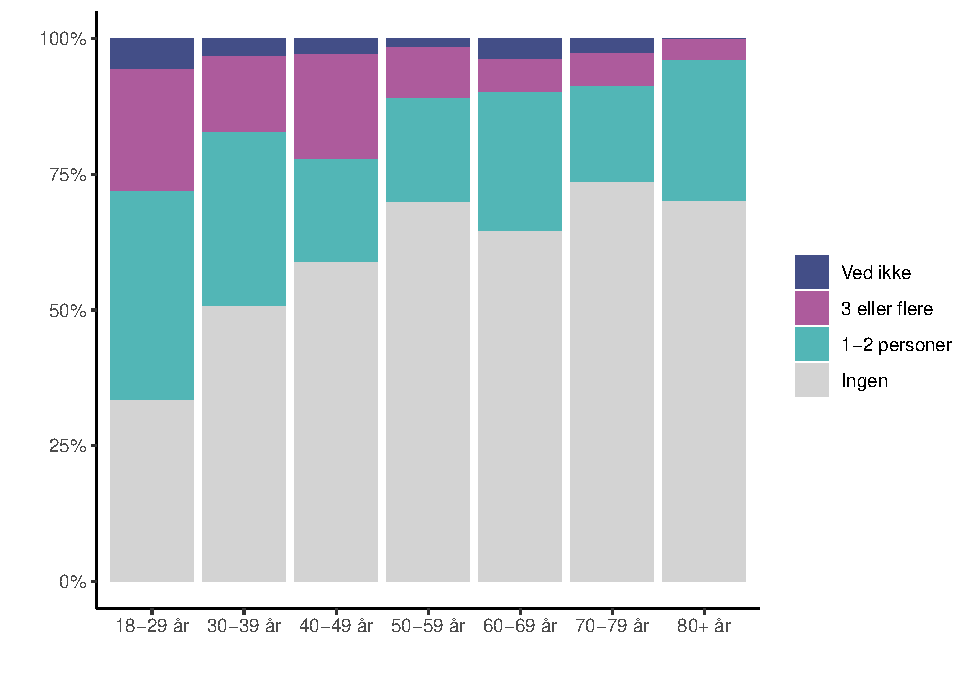
\includegraphics[width=1\linewidth]{en-befolkning-blander-sig_files/figure-latex/fig-6-1-1} \caption{Sammenhængen mellem alder på majoritetsbefolkning og nære venskaber med personer med indvandrerbaggrund. 2022. <br> Note: *Se note til tabel 6.1 for datagrundlag.*}\label{fig:fig-6-1}
\end{figure}

En oplagt forklaring på mønsteret i Figur @(fig:fig-6-1) er, at den yngre del af majoritetsbefolkningen har bedre mulighedsbetingelser for at danne nære venskaber med indvandrere og efterkommere. I en dansk kontekst har J. F. Larsen \& Larsen (\citeproc{ref-larsen2023}{2023}) beregnet andelen af indvandrere og efterkommere i den mulige venskabspulje. Studiet beregner hver enkelt svarpersons mulige venskabspulje som antallet er personer af samme køn, der er fem år yngre/ældre end svarpersonen, og som er bosat i samme boligkvarter, sogn eller kommune som svarpersonen. Logikken er, at der skal være nogle af samme aldersgruppe og af samme køn i et geografisk område før tværetniske venskaber kan opstå.\footnote{Blau har udtrykt det på følgende måde: \emph{''We cannot have Buddhist friends if there are no Buddhist around''} (\citeproc{ref-blau1997}{Peter M. Blau et al., 1997}).} I Figur @(fig:fig-6-2) vises andele af ikke-danske i venskabspuljen på tværs af kommunerne og aldersgrupper. De 18-39-årige svarpersoner, der bor i hovedstadskommunerne, har gode muligheder for at etablere tværetniske venskaber. Andelen af ikke-danske i deres beregnede venskabspulje er i gennemsnit 31 procent, se venstre side i Figur @(fig:fig-6-2). Blandt disse unge har alle en ikke-dansk i deres mulighedspulje, dvs. er ingen med nul procent i, se Figur @(fig:fig-6-2). Omvendt er der heller ikke nogle, hvor med samme alder og køn i deres kommune er ikke-danske, dvs. ingen har 100 procent.

\begin{figure}
\includegraphics[width=1\linewidth]{images/Figur_6_2} \caption{Andelen af indvandrere og efterkommere i majoritetsbefolkningen mulige venskabspulje. Opgjort på kommunalt niveau på tværs af aldersgrupper (A: XX, B: XX) og kommunetype (A: XX, B: XX).}\label{fig:fig-6-2}
\end{figure}

Omvendt ser det ud for de ældre svarpersoner (60 år eller derover), der bor i en landkommune, se højre side af Figur @(fig:fig-6-2) . Andelen af ikke-danske i deres venskabspulje er i gennemsnit kun fire procent. Endvidere er fordelingen venstreskæv, hvilket medfører, at flertallet har under de fire procent---og mange essentielt ingen. Ældre i landkommuner har således begrænsede muligheder for at finde en ven, der ikke har dansk-dansk herkomst. Konklusionen i studiet er således, at den voksne befolkning med dansk-dansk-herkomst har meget forskellige mulighedsstrukturer for at danne venskaber med personer, der ikke har dansk-dansk herkomst. Det skyldes både geografi og det faktum, at indvandrere og efterkommere i gennemsnit er yngre end gruppen med dansk-dansk-herkomst.

J. F. Larsen \& Larsen (\citeproc{ref-larsen2023}{2023}) viser også, at der er en sammenhæng mellem størrelsen af disse venskabspuljer og omfanget af majoritetsbefolkningens venskaber med indvandrere og efterkommere. Dette indikerer, at mulighedsstruktur har betydning for den voksne majoritetsbefolkning. Udtrykt anderledes, fraværet af tværetniske venskaber i nogle kontekster og demografiske segmenter af samfundet er en strukturel betingelse og ikke nødvendigvis et udtryk for bevidst ''venskabsisolation''.

\section{Indvandrere og efterkommeres venskaber med majoriteten}\label{indvandrere-og-efterkommeres-venskaber-med-majoriteten}

Mulighedsstrukturerne for at danne venskaber ser anderledes ud for indvandrere og efterkommere. For minoriteterne er det typiske, at der er rigeligt af mulige majoritetsmedlemmer at danne venskaber med. Det gør sig gældende på skoler, se \hyperref[kap4]{kapitel 4}, og arbejdspladser, se \hyperref[kap5]{kapitel 5}. ''Problemet'' for indvandrere og efterkommere er snarere, at der kan være for få fra deres egen etniske gruppe til at danne sociale relationer med. Det kan gøre det svært at få opfyldt det naturlige ønsket om at finde venner, der ligner sig selv (\citeproc{ref-mcpherson2001}{McPherson et al., 2001}).{[}63{]} Ligesom for majoritetsbefolkningen er indvandreres/efterkommeres venskaber vanskelige at beskrive og studere. C. A. Larsen (\citeproc{ref-calarsen2024}{2024}) har dog brugt ministerielle medborgerskabsundersøgelser til at beskrive ikke-vestlige indvandreres og efterkommers venskaber (blandt voksne, der minimum har levet tre år i Danmark).

Studiet viser, at langt hovedparten af ikke-vestlige indvandrere angiver, at de har en dansk ven. Det er således kun fem procent, der angiver, at de udelukkende har venner med indvandrerbaggrund. Risikoen for en sådan ''venskabsisolation'' er større blandt kvinder, ældre og gruppen med lavere uddannelse og indkomst. Det typiske mønster er, at cirka halvdelen af de ikke-vestlige indvandreres venner har indvandrerbaggrund.\footnote{Målt på andel med indvandrerbaggrund er mønstret igen, at andelen med indvandrerbaggrund er større blandt kvinder, ældre og lavt uddannede, mens der ikke er en selvstændig effekt fra lav indkomst (i modsætning til mønstret for ''venskabsisolation'').} For voksne ikke-vestlige efterkommere angiver kun tre procent, at de udelukkende har venner med indvandrerbaggrund. For disse relativt unge voksne kunne studiet ikke finde sammenhænge mellem baggrundsvariable som køn, alder, uddannelse, indkomst og ''venskabsisolation''. Blandt ikke-vestlige efterkommere er det typiske mønster også, at omkring halvdelen af deres venner har indvandrerbaggrund.\footnote{Måler man på den samlede indvandrerandel blandt vennerne er det eneste klare mønster for efterkommerne, at de højtuddannede har færre venner med indvandrerbaggrund. Der er ikke tydelige sammenhænge med køn, alder og indkomst.}

{[}63{]}: Selvom det er et veletableret menneskeligt forhold, at mennesker har en præference for relationer med andre, der ligner en selv på et eller flere parametre, ved vi ikke hvorvidt indvandrere og efterkommere har større ønske om at etablere venskaber med majoriteten end omvendt. I udgangspunktet kunne man forvente et større ønske om tværetnisk venskab, da indvandrere og efterkommere har stærkere incitamenter til at danne sådanne venskaber, se \hyperref[kap1]{kapitel 1}.

Et centralt spørgsmål i studiet er, hvorvidt størrelsen af egen gruppe påvirker venskabsrelationerne. Størrelsen på egen gruppe er i målt som antallet af indvandrere og efterkommere fra samme oprindelsesland. Indvandrerne kommer fra 122 forskellige lande, mens efterkommerne kommer fra 61 forskellige. Nogle af indvandrerne og efterkommerne har næsten ingen mulighed for at finde venner fra eget oprindelsesland, da de nærmest er de eneste fra et givent land bosat i Danmark. Andre har langt bedre muligheder. Sidstnævnte gælder for eksempel for indvandrere og efterkommere med tyrkisk og syrisk oprindelse, da der er cirka 60.000 personer med tyrkisk og 40.000 med syrisk oprindelse. Studiet viser, at jo større ens egen gruppe er, jo større er andelen af venner med indvandrerbaggrund, og jo mindre er gruppen af venner med dansk baggrund. Størrelsen på egen gruppen forøger også ''risikoen'' for udelukkende at have venner med indvandrerbaggrund. Mønstret ser lidt anderledes ud blandt de ikke-vestlige efterkommere. Det gælder stadig, at jo større antal indvandrere og efterkommere fra deres eget oprindelsesland, jo mindre andel danske venner. Til gengæld er det ikke statistisk sikkert, at et større antal fra samme oprindelsesland påvirker efterkommernes ''risiko'' for udelukkende at have venner med indvandrerbaggrund.

Interessen samler sig ofte om venskabsrelationerne for ikke-vestlige indvandrere og efterkommere. I Udlændinge- og Integrationsministeriets undersøgelser er det kun ikke-vestlige indvandrere/efterkommere, der bliver spurgt. Det efterlader et spørgsmål om, hvorvidt vestlige indvandrere bosat i Danmark egentlig har flere venskabsrelationer med majoritetsbefolkningen end det er tilfældet for ikke-vestlige indvandrere. En ældre undersøgelse fra 2015 kan give en vis indikation. Undersøgelsen blev gennemført blandt voksne (+18) indvandrere fra ti forskellige lande, der havde boet minimum et år i Danmark. Herunder vestlige grupper fra Polen, Rumænien og Spanien, hvor mange var kommet som vandrerne EU-arbejdstagere i perioden fra 2005 og frem, og fra USA og Storbritannien, hvor mange havde levet længere i Danmark. I Figur \ref{fig:fig-6-3} er grupperne arrangeret efter andelen fra de ti grupper, der angiver, at de ingen danske venner har. For alle grupper er der tale om en lille andel, der slet ingen danske venner har. Lægger man andelen, der har ''ingen'' eller kun ''nogle få'' danske venner sammen, så er det indvandrere med kinesisk oprindelse, der har færrest danske venner, se Figur \ref{fig:fig-6-3}. Derefter kommer indvandrerne med rumænsk og filippinsk herkomst. Indvandrerne med britisk og amerikansk oprindelse har flest danske venner. Grupper er vidt forskellige på for eksempel opholdstid, hvilket gør, at man skal være varsom med at sammenligne omfanget af venskaber med majoritetsbefolkningen. Men 2015-undersøgelsen giver en indikation på, at forskelle mellem vestlige og ikke-vestlige indvandrere er begrænset; i det mindste vurderet på andelen uden én eneste ven med dansk baggrund.

\begin{figure}
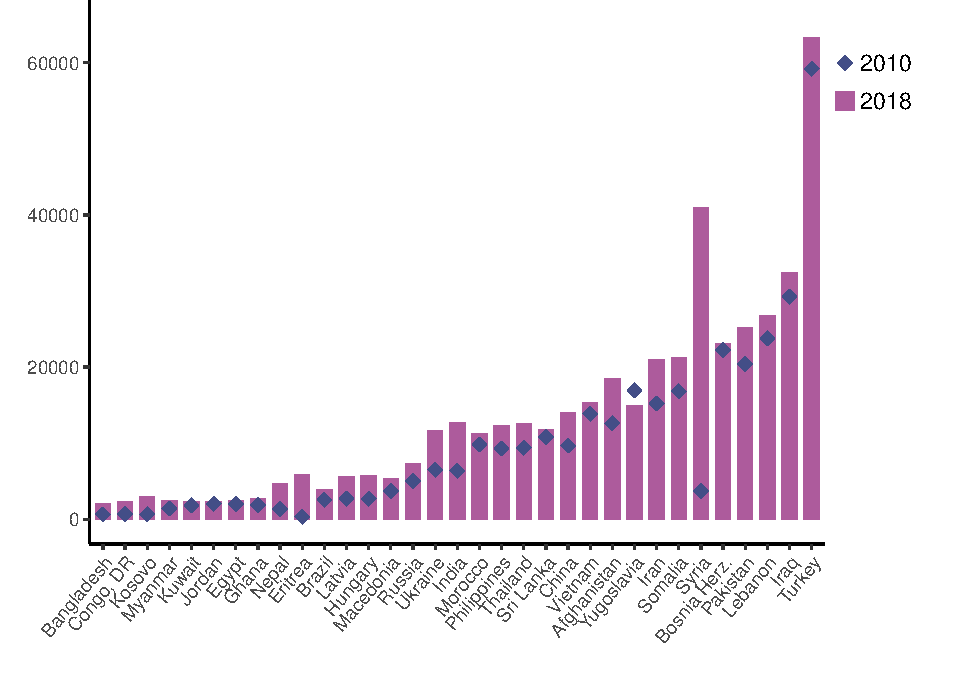
\includegraphics[width=1\linewidth]{en-befolkning-blander-sig_files/figure-latex/fig-6-3-1} \caption{Andel af venner med dansk oprindelse blandt 10 forskellige indvandrergrupper. 2015.}\label{fig:fig-6-3}
\end{figure}

\section{Tværetniske venskaber og deres effekter}\label{tvuxe6retniske-venskaber-og-deres-effekter}

Bogens position er, at venskaber nok er svære at studere, men ikke desto mindre er de værd at beskæftige sig med. Etablering af venskaber mellem majoriteten og indvandrere/efterkommere er den oplagte første tværetniske social relation og der er mange indikationer på, at sådanne venskabsrelationer kan have effekter. Figur \ref{fig:fig-6-4} og Figur \ref{fig:fig-6-5} illustrerer sammenhængen mellem venskabsrelationer og fordomme på danske data.

\begin{figure}
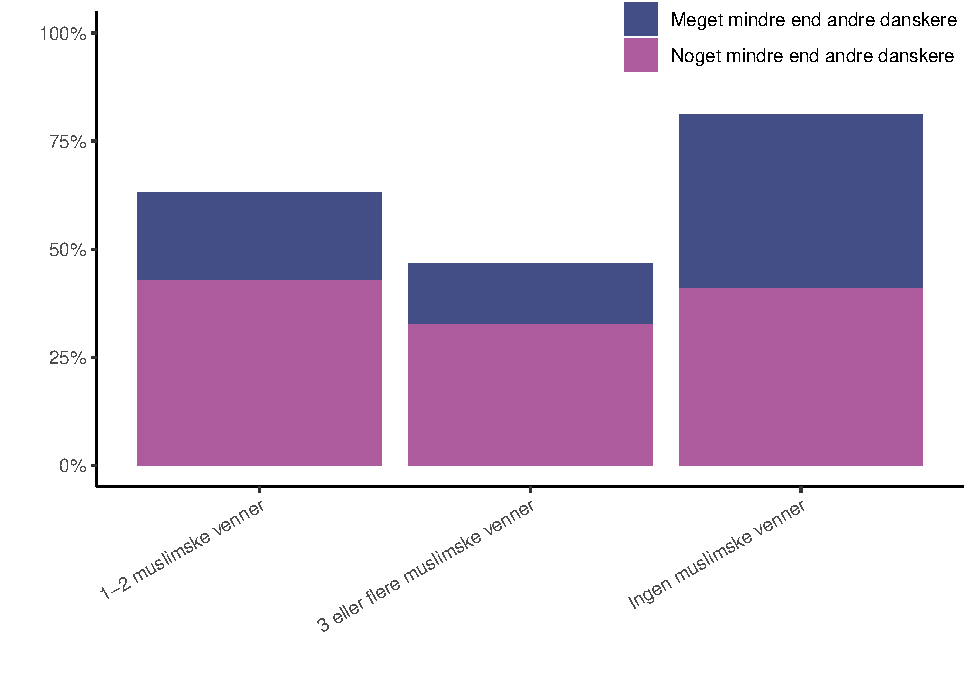
\includegraphics[width=1\linewidth]{en-befolkning-blander-sig_files/figure-latex/fig-6-4-1} \caption{Majoritetens vurdering af, hvorvidt muslimer i Danmark identificerer sig mindre med landet end andre danskere. Opdelt på antal muslimske venner.}\label{fig:fig-6-4}
\end{figure}

Figur \ref{fig:fig-6-4} viser, at majoritetsbefolkningen uden én eneste muslimsk ven er langt mere tilbøjelig til at svarere, at muslimer i Danmark identificerer sig mindre med Danmark. 40 procent siger ''meget mindre'' og 41 procent siger ''noget mindre''. Blandt majoritetsbefolkningen, der har tre eller flere venner med muslimsk baggrund, er de tilsvarende andele 15 og 28 procent. Figur \ref{fig:fig-6-5} viser en lignende sammenhæng mellem det at have muslimske venner og opfattelsen af, at muslimer i Danmark bekymrer sig mindre om andre danskere.

\begin{figure}
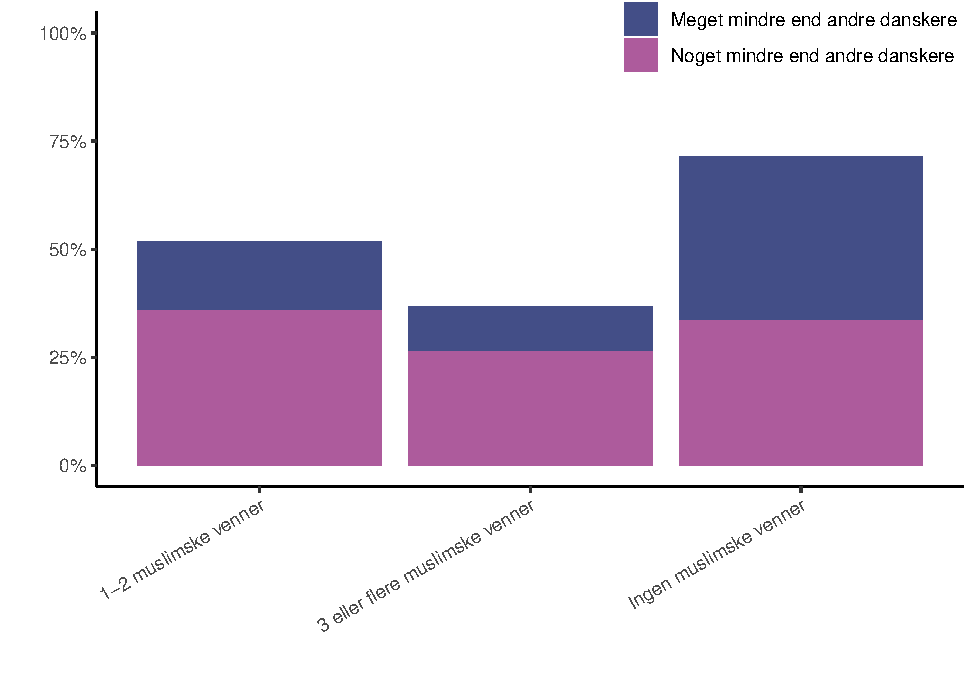
\includegraphics[width=1\linewidth]{en-befolkning-blander-sig_files/figure-latex/fig-6-5-1} \caption{Majoritetens vurdering af, hvorvidt muslimer i Danmark bekymrer sig mindre om andre danskernes anliggender og behov. Opdelt på antal muslimske venner.}\label{fig:fig-6-5}
\end{figure}

Man skal dog tage sammenhænge mellem venskabsrelationer og fordomme med en række forbehold. Det vigtigste er, at kausaliteten kan gå begge veje. Venskaber kan lede til færre fordomme, for eksempel om muslimer i Danmark, men færre fordomme kan også lede til flere venskaber med den muslimske minoritet. Problemer med at isolere den kausale effekt fra venskabsrelationer diskuteres i næste \hyperref[kap7]{kapitel}.

Vi opfatter de præsenterede studier som et første skridt i et spirende forskningsfelt. Deres ydmyge bidrag er at påpege, at størrelsesforhold har effekt på tværetniske venskabsrelationer. På grund af alder og geografi har dele af majoritetsbefolkningen begrænsede muligheder for at etablere venskaber med indvandrere/efterkommere. Andre har bedre mulighedsstrukturer. Det gælder de unge og dem i byerne. Det gør (tilsyneladende) en forskel for sandsynligheden for at have en ven med indvandrerbaggrund. Selv blandt dem, der mener, at indvandring er et problem for Danmark (\citeproc{ref-larsen2023}{J. F. Larsen \& Larsen, 2023}). Indvandrere og efterkommere er ikke på samme måde begrænset af, at der ikke er danskere nok. Men antallet fra eget hjemland kan virke som en begrænsning på deres venskabsmuligheder, hvilket for indvandrere tilsyneladende øger sandsynligheden for at etablere venskaber med majoritetsbefolkningen. Effekten er dog svag og kunne ikke findes for efterkommerne. Mens tværetniske partnerskaber er undtagelsen, se \hyperref[kap2]{kapitel 2}, så vidner ovenstående om, at tværetniske venskaber er typiske. Venskab er det naturlige første skridt.

\chapter{Integration i et kontaktperspektiv}\label{kap7}

\emph{\href{https://vbn.aau.dk/en/persons/albrekt}{Christian Albrekt Larsen}}

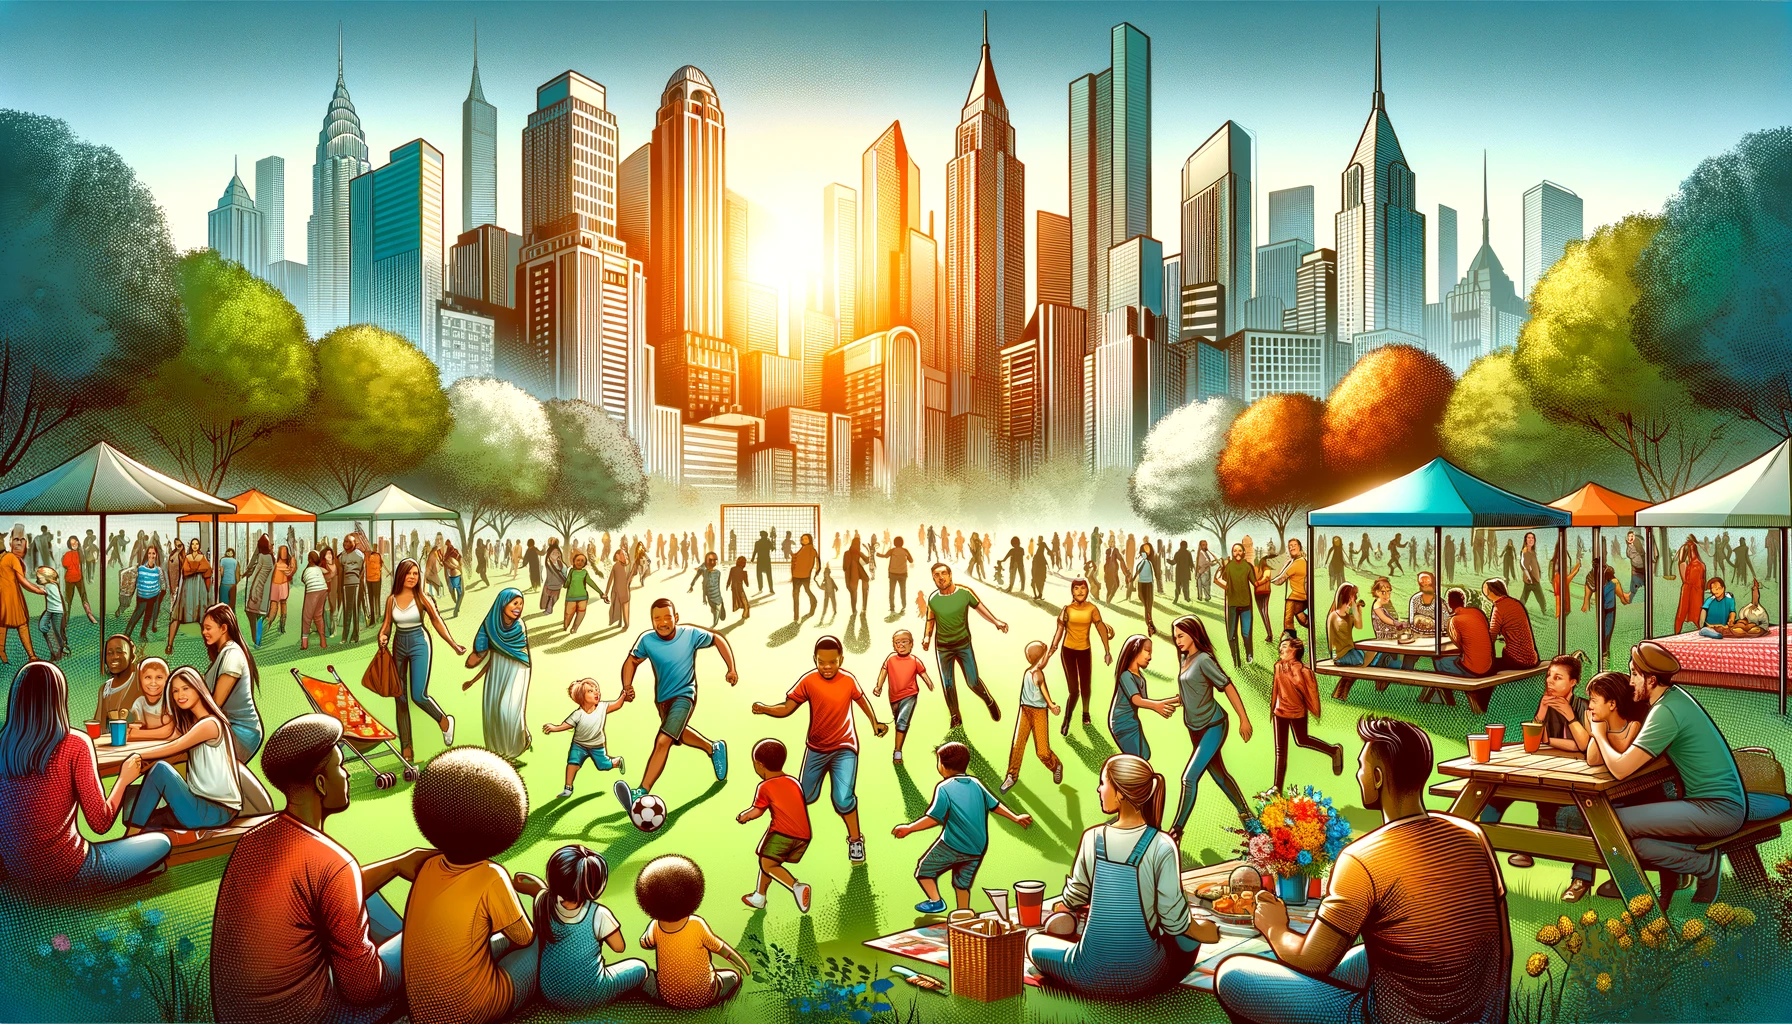
\includegraphics[width=1\linewidth]{images/dalle-integration}

''En befolkning blander sig'' er inspireret af den lange amerikanske sociologiske forskningstradition, der handler om, hvordan indvandrere klarede sig i USA, og hvordan det formåede USA som nation. Udgangspunktet for meget af den amerikanske forskning er, at integrationen/assimileringen i det store hele lykkes. Ikke blot for den enkelte indvandrer og hendes efterkommere, men også for USA som samfund. Opgaven for de tidlige amerikanske sociologer var således været at forklare, hvorfor det var gået så godt. Hvad var de magiske ingredienser i den amerikanske smeltedigel? Udgangspunktet for meget af den samtidige europæiske forskning om integration er anderledes. Vi lever et samfund, hvor grundfortællingen er, at integrationen i det store hele er mislykkes. Det gør i særdeleshed gældende i Danmark. En nærlæsning af de politiske partiprogrammer viser, at fra den yderste højrefløj til den yderste venstrefløj er man enige om, at integrationen er mislykkes (\citeproc{ref-nielsen2024}{\textbf{nielsen2024?}}). Uenigheden starter først, når det kommer til løsningsforslagene. Det omgivende samfund er således typisk interesseret i en forklaring på, hvorfor integrationen er mislykkes, og hvad man kan gøre ved det. Det bliver tit til et spørgsmål om, hvad den enkelt indvandrer eller efterkommer gør galt, hvad majoritetsbefolkningen gør galt eller, hvad der er galt med samfundsindretningen. I bogen har vi forsøgt at løfte spørgsmålet om integration udover denne øvelse i fejlfinding og problemløsning. I tråd med den amerikanske tradition har forfatteren til denne bog mere været interesseret i de positive forklaringer på, hvordan integration egentlig foregår. Bogens bud er, at ansigt-til-ansigt møder mellem majoriteten og minoriteter er en vigtig forudsætning for integration.

I det afsluttende kapitel diskuteres dette fokus på ansigt-til-ansigt møder, som jeg sammenfattende vil kalde et kontaktperspektiv. I det første afsnit diskuterer jeg, hvorledes kontaktperspektivet adskiller sig fra andre perspektiver på integration, der ofte florerer i den offentlige danske debat. I det andet afsnit diskuterer jeg med udgangspunkt i bogens resultater, hvorledes kontaktperspektivet \emph{ikke} leverer nogen nem løsning på integration. Bogens udgangspunkt er, at et kan være vanskeligt at etablere tværetniske ansigt-til-ansigt-møder. Og hvis de etableres, er der ikke garanti for, at det leder til etablering af sociale relationer og reduktion i fordomme. I det tredje afsnit beskriver jeg specifikt resultaterne fra to studier fra det underliggende forskningsprojekt, hvor vi har studeret effekterne af at mødes på arbejdspladsen. I det fjerde afsnit diskuterer jeg nogle af kontaktperspektivets begrænsninger og peger på fremtidig forskning, der kan bringe os nærmere en solid forståelse af integrationsprocesserne i Danmark.

\section{Kontaktperspektivet og debatten om integration}\label{kontaktperspektivet-og-debatten-om-integration}

Den danske debat om integration lider ofte under, at man ikke er enige om, hvad vi snakker om. Forud for integrationsloven fra 1998 havde vi for eksempel en ekspertgruppe, der skulle lave et grundlag for loven. Kommissionen sprang dog lidt over, hvor gæret var lavest. De skrev simpelthen, at de havde forskellige opfattelser af integration.\footnote{''Udvalget har drøftet de forskellige politiske og teoretiske opfattelser om integration og integrationspolitik. Nogle udvalgsmedlemmer lægger større vægt på kulturelle faktorer i integrationsprocessen, mens andre særligt fremhæver sociale faktorer. Andre igen opfatter integration som en samlebetegnelse for en række konkrete tiltag og finder det mere nyttigt at anvende betegnelsen etnisk ligestilling.'' (Betænkning nr. 1337, Integration. Betænkning afgivet af det af indenrigsminsteren nedsatte Integrationsudvalg, s. 70).} Med den tilføjelse, at en definition nok ikke var nødvendig for at diskutere praktiske tiltag.\footnote{''udvalget er af den opfattelse, at fastlæggelsen af en overordnet forståelse af et integrationsbegreb ikke altid vil være afgørende for drøftelsen af de praktiske enkeltspørgsmål, som opstår i forbindelse med tilrettelæggelsen af integrationsindsatsen (Betænkning nr. 1337, Integration. Betænkning afgivet af det af indenrigsminsteren nedsatte Integrationsudvalg, s. 71).} Det er måske rigtigt. Men det er nu heller ikke praktisk, at vi i mere end to årtier ikke rigtigt ved, hvad vi snakker om. Handler det om integration af det danske samfund eller handler det om, hvornår den enkelte indvandrer eller efterkommer er integreret? Handler det om danskerne og indvandrere eller handler det kun om indvandrerne? Handler det om deltagelse på arbejdsmarkedet, uddannelse, bopæl og kriminalitet? Handler det om følelsen af være dansk? Eller handler det om, at man synes det samme? I Udlændinge og integrationsministeriets såkaldte integrationsbarometer er den pragmatiske løsning, at det nok handler lidt om det hele. Så man måler lidt tilfældigt på forskellige ting. Så kan man tage for sig af resultaterne, som man vil. Problemet med manglende definitioner er blot blevet forværret i den danske diskussion om parallelsamfund. I den første Redegørelse for parallelsamfund i 2019 skrev den ministerielle arbejdsgruppe '' Begrebet parallelsamfund kan have forskellig betydning, men er i denne redegørelse et samfund, som er fysisk eller mentalt isoleret og følger egne normer og regler, uden nogen nævneværdig kontakt til det danske samfund og uden ønske om at blive en del af det
danske samfund.'' (\citeproc{ref-oim2019}{Økonomi og Indenrigsministeret, 2019}: 37). Herefter gik man i gang med at beskrive den boligmæssige koncentration, der ikke havde et eneste mål for tværetniske kontakter. Dog med en tilføjelse om, at nok ikke var helt optimalt.\footnote{''En stor koncentration af bestemte befolkningsgrupper, som det er tilfældet i boligområderne på ghettolisten, er sandsynligvis med til at forstærke eksistensen af parallelsamfund. Men i sagens natur handler parallelsamfund om det enkelte individs identitet og værdigrundlag. Derfor er det umuligt at komme med et præcist, statistisk bud på, hvor mange personer med ikke-vestlig baggrund der reelt lever i parallelsamfund i Danmark'' (\citeproc{ref-oim2019}{Økonomi og Indenrigsministeret, 2019}: 37).} For nogle akademikere er den principielle løsning på de manglende definitioner at dekonstruere det hele. Hvis vi ikke ved, hvad vi snakker om, så er det en kærkommen lejlighed til at droppe integrationsdiskussionen. Bogens udgangspunktet har været et andet. Integration er en helt central proces for at etablere et samfund, der både er godt for både nye og gamle danskere. Det er også en term, der kan defineres, se \hyperref[kap1]{kapitel 1}, og det er en proces, der kan studeres med almindelige samfundsfaglige data og metoder.

Vores definition af integration følger Alba og Nee, der jævnfør \hyperref[kap1]{kapitel 1} definerer assimilation/integration ''som nedgang i betydning af en etnisk distinktion og dens forbundne kulturelle og sociale forskelle. Hvor ''nedgang'' fortolkes således, at den etniske distinktion fremtræder mindre og aftager i relevans for færre og færre domæner af det sociale liv'' (\citeproc{ref-alba1997}{1997}: 863, egen oversættelse). Integration er således mere end bare, at minoriteter ligner majoriteten. Det er ikke uinteressant om minoriteter har samme uddannelses-, beskæftigelses- og indkomstniveau som majoritetsbefolkning. Det er heller ikke uinteressant om minoriteter har samme værdier og holdninger som majoritetsbefolkningen. Det er en indikation på, at betydningen af etniske distinktioner er begrænset i flere domæner af det sociale liv. Men i princippet kan man godt have en situation, hvor minoriteter og majoriteter ligner hinanden på en lang række parametre, men aldrig mødes med hinanden. Et sådan samfund vil være præget af etniske skillelinjer, der nemt kan reducere tolerance, solidaritet og tillid. Derfor er man i et kontaktperspektiv optaget af, hvorvidt der reelt er ansigt-til-ansigt-møder mellem majoriteten og minoriteter. Men der er tale om et samfundsperspektiv. Det handler således \emph{ikke} om, hvad det enkelte individ skal gøre for at være (nok) integreret. Det handler snarere om, hvordan moderne samfund hænger sammen. Alle indvandre- og efterkommere behøver ikke at have en ven fra majoritetsbefolkningen. Og alle i majoritetsbefolkningen behøver ikke at have en ven med indvandrerbaggrund. Men findes der ingen tværetniske venskaber, så vil man i et kontaktperspektiv mene, at samfundet har et integrationsproblem.

Den klassiske kritik af den amerikanske assimileringsforskning er, at majoriteten bruges som ideal og bliver en standard for, hvordan indvandrere og efterkommere skal opføre sig, og hvad de skal mene. Bogens forfattere er enige i, at det er en problematisk tilgangsvinkel til studiet af integration. Ved at studere tilstedeværelsen af tværetniske sociale relationer, og fravær er tværetniske fordomme, kan man undgå tendensen til at gøre majoriteten til en standard, som minoriteter skal opvejes imod.

\section{De svære ansigt-til-ansigts-møder}\label{de-svuxe6re-ansigt-til-ansigts-muxf8der}

At majoriteten og minoriteter mødes ansigt-til-ansigt kan man ikke tage for givet. I \hyperref[kap1]{kapitel 1} beskrev vi, hvordan mennesker synes at have et iboende ønske og at omgås mennesker, der ligner dem selv. I \hyperref[kap2]{kapitel 2} beskrev vi, hvorledes den mekanisme afspejler sig i partnerskaber. Langt de fleste med dansk herkomst er partnere mere andre med dansk herkomst. Og langt de fleste indvandrere finder partnere fra eget oprindelsesland. Tidligere forskning har også vist, hvordan indvandrere og efterkommere bosætter sig blandt andre indvandrere og efterkommere, og hvordan gruppen med dansk herkomst, bosætter blandt andre med dansk herkomst. Bogen titel, ''En befolkning blander sig'', er således lidt et ordspil med en tidligere bog fra Rockwool Fondens Forskningsenhed (\citeproc{ref-damm2006}{Damm et al., 2006}), der bar titlen ''En befolkning deler sig op?'' Efterfølgende analyser af bosætningsmønstre har vist, at den etniske opdeling steg frem til slutningen af 1990'erne, hvorefter den har været faldende på landsplan (\citeproc{ref-damm2022}{Damm et al., 2022}). Endeligt er det velkendt, at indvandrere og efterkommere deltager markant mindre i frivillige organisationer end majoritetsbefolkningen {[}Jørgensen \& Qvist (\citeproc{ref-jorgensen2023}{2023}); @ jorgensen2024{]}. Der er således mange historiske og samtidige eksempler på, at tværetniske møder ikke kan tages for givet.

Derfor har bogen, jævnfør \hyperref[kap1]{kapitel 1}, været optaget af arenaer, hvor befolkningsgrupper med forskellig etnisk oprindelse ikke kan undgå at møde hinanden. Det gør sig gældende for det voksende antal blandede børn beskrevet i \hyperref[kap3]{kapitel 3}. De hænger så at sige på deres forældre og deres bredere familier. Det gør sig i nogen grad også gældende for grundskoler, hvor man ikke har frit valg til at vælge klassekammerater. I de større danske byer, men specielt i København, er der et skolelandskab, de gør det muligt for nogle forældre at vælge barnets klassekammerater, som beskrevet i \hyperref[kap4]{kapitel 4}. Kapitlet beskrev også, hvordan det primært sker via den boligmæssige placering inden barnet starter i skole. Det reducerer tværetniske ansigt-til-ansigt-møder. Men i et det mest af landet er det vanskeligt for majoriteten ikke at mødes med indvandrere og efterkommere, og visa versa, i de danske grundskoler. \hyperref[kap4]{Kapitel 4} viste, at på landsplan er den etniske opdeling af danske grundskole støt faldende. En central pointe fra kapitel 4 var således, at den videre debat derfor må skelne mellem to dimensioner: Den store nationale skala, som måske kan bidrage til en meget generel fortælling om samfundstilstanden i Danmark, og den kommunale skala, hvor lokale og specifikke processer finder sted, men som ikke nødvendigvis kan generaliseres til at udtrykke en samfundsdiagnose. Endeligt viste \hyperref[kap5]{kapitel 5}, at de danske arbejdspladser er blevet en central arena for tværetniske møder i den voksne befolkning. \href{kap5}{Kapitel 5} viste, at danske arbejdspladser godt nok bliver mere etnisk opdelte. Men det til trods, er der sket en markant stigning i majoritetsbefolkning, der deler arbejdsplads med indvandrere og efterkommere. Deraf bogens titel, ''En befolkning blander sig''.

Det næste problem er dog, at ansigt-til-ansigt møder ikke nødvendigvis leder til sociale relationer og nedbrydning af fordomme om de andre. I \hyperref[kap1]{kapitel 1} blev det beskrevet, hvordan socialpsykologien har vist, at positive ind-gruppe-, og negative ud-gruppe-forestillinger også er en fast bestanddel af den menneskelige natur. Derfor krævede det en vis kvalitet og intensitet i ansigt-til-ansigt møder, hvis fordomme skulle reduceres. Det var den anden grund til, at bogen har været optaget af familier, skoler og arbejderpladser. Det er mødepladser, hvor ansigt-til-ansigt møderne ofte vil være ganske intense. I modsætning til mere flygtige møder i bybilledet, i boligkvarterer og i visse dele af foreningslivet.

Bogen har vist, at tværetniske ansigt-til-ansigt møder er blevet hyppigere i familier, grundskoler og på arbejdspladser. I \hyperref[kap6]{kapitel 6} viste bogen også, at tværetniske venskaber er udbredte både blandt majoritetsbefolkningen og blandt minoriteter. Sammenhængen mellem at blive eksponeret til en udgruppe og etableringen af venskabsrelationer, eller reduktion i fordomme, er dog et spirende forskningsfelt, hvor det er svært at drage faste konklusioner. I det underliggende forskningsprojekt har i første omgang studeret effekterne af at mødes på arbejdspladser. Her synes det mest åbenbart, at ansigt-til-ansigt-møder både kan forøge og reducere betydningen af etniske skillelinjer.

\section{Effekter fra at mødes på arbejdspladsen}\label{effekter-fra-at-muxf8des-puxe5-arbejdspladsen}

Diop-Christensen \& Larsen (\citeproc{ref-diopchristensen2024}{2024}) viser, at hvis der er mange østeuropæiske indvandrere på en arbejdsplads, så stiger modstanden mod indvandringen fra østeuropæiske lande. Men det gælder kun for danske medarbejdere, der har usikre jobs (opgjort som ansat på det sekundære arbejdsmarked i den private sektor). For danske medarbejdere med sikker beskæftigelse gør det ingen forskel på modstanden mod østeuropæiske indvandring, hvorvidt der er få eller mange på ens egen arbejdsplads. Dernæst viser studiet, at når danskere i sikker beskæftigelse deler arbejdsplads med mange ikke-vestlige indvandrere/efterkommere, så falder modstanden mod indvandring fra fattige lande udenfor Europa. Høj eksponering på arbejdspladsen er således ikke altid sammenfaldene med mere positive holdninger til indvandring hos majoritetsbefolkningen. Eksponeringen er formentligt mest effektfuld, når der er betydelige fordomme at nedbryde og når majoriteten oplever, at deres egen beskæftigelse er sikker. Men det er mekanismer, der trænger til at blive yderligere belyst.

Diop-Christensen et al. (\citeproc{ref-diopchristensen2024b}{2024}) viser, at (ikke-vestlige) indvandrere/efterkommere, der har mange kolleger med dansk herkomst, føler sig mere danske end indvandrere/efterkommere, der har færre kolleger med dansk herkomst. Det gælder også, når man kontrollerer for en lang række andre forhold, der også kunne have betydning (antal år levet i Danmark, etnisk komposition af boligområde, statsborgerskab etc.). Det støtter kontaktperspektivet. Men studiet viser også, at sammenhængen mellem eksponering til majoriteten på arbejdspladsen og følelsen af være dansk kun er gældende for de indvandrere og efterkommere, der ikke føler sig diskrimineret på arbejdsmarkedet. For gruppen, der føler sig diskrimineret, finder studiet den omvendte sammenhæng. Mere eksponering på arbejdspladsen hænger for disse indvandrere sammen med \emph{mindre} følelse af at være dansk. Det vidner om, at et stigende antal danske kolleger ikke altid giver indvandrere og efterkommere en følelse af at være dansk. Mødet på arbejdspladsen virker formentlig bedst, hvis indvandrere og efterkommere føler, at majoritetsbefolkningen behandler dem på lige fod med andre kolleger.

\section{Kontaktperspektivets begrænsninger og videre forskning}\label{kontaktperspektivets-begruxe6nsninger-og-videre-forskning}

Det underliggende forskningsprojekt har fokuseret på arbejdspladserne og ikke nærmere studeret, hvad der sker i blandede familier\footnote{H..Y. Qvist, J.Y. Qvist og M. Dahlberg arbejder dog på at færdiggøre et studie om, hvorledes tværetnisk partnerskab påvirker politisk deltagelse.} og i blandede skoler. Der er dog et spirende forskningsfelt om venskabsrelationerne i skoleklasser. I det dominerede europæiske studie af klasserum bedes eleverne nominere deres bedste venner i klassen (op til maksimalt fem stk.).\footnote{Children of immigrants longitudional survey in four European Countries'' Home -- Cils4eu} Sådanne klasserumsdata er indsamlet i Tyskland, Holland, Storbritannien, Sverige og Norge. Det giver mulighed for 1) at beregne venskaber, hvor begge partner nominerer hinanden, 2) at få nøjagtig information om vennens etnicitet, og 3) lave beregner på selve netværket i stedet for på personerne.

Et af hovedresultaterne fra skolerumsdata er, at der er etniske opdelinger internt i skoleklasser. Børn med majoritetsbaggrund i Tyskland, Holland, Storbritannien og Sverige har typisk bedste venner i klassen, der også har majoritetsbaggrund. Analyser på de europæiske skolerumsdata også viser, at det både skyldes, at der er en præference for sådanne etnisk homogene venskaber, jævnfør \hyperref[kap1]{kapitel 1}, og det simple forhold, at majoriteten netop er en majoritet (se Van Tubergen \& Smith (\citeproc{ref-tubergen2018}{2018}) for et overblik). Omvendt har indvandrerbørn i blandede klasser ofte tendens til at danne venskaber med andre indvandrerbørn. To mindre kvalitative danske undersøgelser i etnisk diverse syvendeklaser (\citeproc{ref-jensen2018}{Jensen, 2018}) førsteklasser (\citeproc{ref-vertelyte2019}{Vertelyte, 2019}) indikerer også, at børn af majoritetsbefolkningen primært er venner med andre børn af majoritetsbefolkningen.

At venskabsnetværk er etnisk opdelte på ''tvungne'' mødepladser er dog ikke ensbetydende med, at ansigt-til-ansigt-møderne ikke betyder noget. Det må bedømmes ved at sammenligne venskabsnetværk i mere og mindre etniske diverse kontekster, hvilket vi desværre ikke har danske data på. Hverken på skoler eller arbejdspladser. Samtidigt er der tale om ganske komplekse mekanismer. Tyske skolerumsdata, der følger den samme klasse over tid, viser for eksempel, at elever med stærke etniske identiteter finder sammen, men samtidigt undgår elever fra samme gruppe med svage etniske identiteter, da de kan virke truende for gruppen (\citeproc{ref-leszczensky2019}{Leszczensky \& Pink, 2019}). Der er således undergrupper af børn med svagere etniske identiteter, der danner tværetniske venskaber. Tilsvarende viser svenske data, der følger klasser over tid, at hvis den etniske opdeling (i etniske blandede klasser) er lav i udgangspunktet, så stimulerer det til dannelse af endnu flere tværetniske venskaber (\citeproc{ref-zhao2023}{Zhao, 2023}). Endeligt kan ansigt-til-ansigt møderne godt skabe tolerance og tillid, selvom venskabsrelationer forbliver segrerede. Et dansk tillidseksperiment i henholdsvis etnisk diverse og homogene 8. klasser viste for eksempel, at hudfarve betød mindre i de blandede skolede (\citeproc{ref-larsen2013}{C. A. Larsen et al., 2013}). Effekterne af tværetniske møder i grundskolerne er et oplagt fremtidigt dansk forskningsfelt. Et andet oplagt forskningsfelt er, hvordan det kommer til at gå de børn etnisk blandet herkomst, som vi beskrev i \hyperref[kap2]{kapitel 2}. Dem ved vi stort set intet om, da kategorien ikke findes i de danske statistikker. Ikke desto mindre er det vores forventning, at lige præcis den gruppe vil rokke grundlæggende ved vores forestillinger om ''os'' og ''dem''.

\chapter*{Litteraturliste}\label{litteraturliste}
\addcontentsline{toc}{chapter}{Litteraturliste}

\phantomsection\label{refs}
\begin{CSLReferences}{1}{0}
\bibitem[\citeproctext]{ref-alba1997}
Alba, R., \& Nee, V. (1997). Rethinking assimilation theory for a new era of immigration. \emph{International Migration Review}, \emph{31}(4), 826--874.

\bibitem[\citeproctext]{ref-allen2007}
Allen, R., \& Vignoles, A. (2007). What should an index of school segregation measure? \emph{Oxford Review of Education}, \emph{33}(5), 643--668. \url{https://doi.org/10.1080/03054980701366306}

\bibitem[\citeproctext]{ref-allport1954}
Allport, G. W. (1954). \emph{The nature of prejudice} (1st ed.). Addison-Wesley Pub. Co.

\bibitem[\citeproctext]{ref-andersen2019a}
Andersen, H. S. (2019). \emph{Ethnic spatial segregation in european cities}. Routledge.

\bibitem[\citeproctext]{ref-andersen2019}
Andersen, S. C., \& Guul, T. S. (2019). Reducing minority discrimination at the front line---combined survey and field experimental evidence. \emph{Journal of Public Administration Research and Theory}, \emph{29}(3), 429--444. \url{https://doi.org/10.1093/jopart/muy083}

\bibitem[\citeproctext]{ref-andersson2021}
Andersson, H., \& Dehdari, S. H. (2021). Workplace contact and support for anti-immigration parties. \emph{American Political Science Review}, \emph{115}(4), 1159--1174.

\bibitem[\citeproctext]{ref-uxe5slund2010}
Åslund, O., \& Skans, O. N. (2010). Will i see you at work? Ethnic workplace segregation in sweden, 1985--2002. \emph{ILR Review}, \emph{63}(3), 471--493.

\bibitem[\citeproctext]{ref-bell1954}
Bell, W. (1954). A probability model for the measurement of ecological segregation. \emph{Social Forces}, \emph{32}(4), 357--364. \url{https://doi.org/10.2307/2574118}

\bibitem[\citeproctext]{ref-blau1994}
Blau, P. M. (1994). \emph{Structural contexts of opportunities}. University of Chicago Press.

\bibitem[\citeproctext]{ref-blau1984a}
Blau, P. M., Beeker, C., \& Fitzpatrick, K. M. (1984). Intersecting social affiliations and intermarriage. \emph{Social Forces}, \emph{62}(3), 585--606.

\bibitem[\citeproctext]{ref-blau1997}
Blau, Peter M., Schwartz, J. E., \& Blau, P. M. (1997). \emph{Crosscutting social circles: Testing a macrostructural theory of intergroup relations}. Routledge. \url{https://doi.org/10.4324/9781351313049}

\bibitem[\citeproctext]{ref-boterman2019}
Boterman, W., Musterd, S., Pacchi, C., \& Ranci, C. (2019). School segregation in contemporary cities: Socio-spatial dynamics, institutional context and urban outcomes. \emph{Urban Studies}, \emph{56}(15), 3055--3073. \url{https://doi.org/10.1177/0042098019868377}

\bibitem[\citeproctext]{ref-bunar2010}
Bunar, N. (2010). The geographies of education and relationships in a multicultural city: Enrolling in high-poverty, low-performing urban schools and choosing to stay there. \emph{Acta Sociologica}, \emph{53}(2), 141--159. \url{https://doi.org/10.1177/0001699310365732}

\bibitem[\citeproctext]{ref-butler2007}
Butler, T., \& Hamnett, C. (2007). The geography of education: introduction. \emph{Urban Studies}, \emph{44}(7), 1161--1174. \url{https://doi.org/10.1080/00420980701329174}

\bibitem[\citeproctext]{ref-carrington1997}
Carrington, W. J., \& Troske, K. R. (1997). On measuring segregation in samples with small units. \emph{Journal of Business \&Amp; Economic Statistics}, \emph{15}(4), 402--409. \url{https://doi.org/10.1080/07350015.1997.10524718}

\bibitem[\citeproctext]{ref-damm2022}
Damm, A. P., Hassani, A., Tranæs, T., \& Schultz-Nielsen, M. L. (2022). \emph{Bosætning i danmark: I et 35-årigt perspektiv}. Syddansk Universitetsforlag.

\bibitem[\citeproctext]{ref-damm2006}
Damm, A. P., Schultz-Nielsen, M.-L., \& Tranæs, T. (2006). \emph{En befolkning deler sig op?} Gyldendal.

\bibitem[\citeproctext]{ref-diopchristensen2024b}
Diop-Christensen, L. E., Hedegaard, T. F., \& Diop-Christensen, A. (2024). Is employment enough? Exposure to natives at work and immigrants' cultural assimilation. \emph{Acta Sociologica}.

\bibitem[\citeproctext]{ref-diopchristensen2024}
Diop-Christensen, L. E., \& Larsen, C. A. (2024). Working together or apart? Exposure between natives and migrants at danish workplaces from 1996 to 2019. \emph{Journal of Ethnic and Migration Studies}.

\bibitem[\citeproctext]{ref-epinion2017}
Epinion. (2017). \emph{Frit skolevalg---hovedrapport}. Undervisningsministeriet.

\bibitem[\citeproctext]{ref-farley1984}
Farley, J. E. (1984). P* segregation indices: What can they tell us about housing segregation in 1980? \emph{Urban Studies}, \emph{21}(3), 331--336. \url{https://doi.org/10.1080/00420988420080591}

\bibitem[\citeproctext]{ref-forbes2004}
Forbes, H. D. (2004). Ethnic conflict and the contact hypothesis. In \emph{The psychology of ethnic and cultural conflict} (pp. 69--88).

\bibitem[\citeproctext]{ref-fossett2017}
Fossett, M. (2017). \emph{New methods for measuring and analyzing segregation}. \url{https://doi.org/10.1007/978-3-319-41304-4}

\bibitem[\citeproctext]{ref-frankel2011}
Frankel, D. M., \& Volij, O. (2011). Measuring school segregation. \emph{Journal of Economic Theory}, \emph{146}(1), 1--38. \url{https://doi.org/10.1016/j.jet.2010.10.008}

\bibitem[\citeproctext]{ref-thomsen2012}
Frølund Thomsen, J. P. (2012). How does intergroup contact generate ethnic tolerance? The contact hypothesis in a scandinavian context. \emph{Scandinavian Political Studies}, \emph{35}(1), 159--178.

\bibitem[\citeproctext]{ref-glitz2014}
Glitz, A. (2014). Ethnic segregation in germany. \emph{Labour Economics}, \emph{29}, 28--40.

\bibitem[\citeproctext]{ref-gorard2002}
Gorard, S., \& Taylor, C. (2002). What is segregation?: A comparison of measures in terms of {``strong''} and {``weak''} compositional invariance. \emph{Sociology}, \emph{36}(4), 875--895. \url{https://doi.org/10.1177/003803850203600405}

\bibitem[\citeproctext]{ref-gordon1964}
Gordon, M. M. (1964). \emph{Assimilation in american life: The role of race, religion, and national origins}. Oxford University Press.

\bibitem[\citeproctext]{ref-harris2017}
Harris, R. (2017). Measuring the scales of segregation: Looking at the residential separation of white british and other schoolchildren in england using a multilevel index of dissimilarity. \emph{Transactions of the Institute of British Geographers}, \emph{42}(3), 432--444. \url{https://www.jstor.org/stable/45147105}

\bibitem[\citeproctext]{ref-hassan2022}
Hassan, S., Hvidtfeldt, C., Andersen, L. H., \& Udsen, R. O. (2022). Do refugee children impair the academic performance of native children in the school? Informative null results from danish register data. \emph{European Sociological Review}, \emph{39}(3), 352--365. \url{https://doi.org/10.1093/esr/jcac059}

\bibitem[\citeproctext]{ref-hermansen2015}
Hermansen, A. S., \& Birkelund, G. E. (2015). The impact of immigrant classmates on educational outcomes. \emph{Social Forces}, \emph{94}(2), 615--646. \url{https://doi.org/10.1093/sf/sov073}

\bibitem[\citeproctext]{ref-james1985}
James, D. R., \& Taeuber, K. E. (1985). Measures of segregation. \emph{Sociological Methodology}, \emph{15}. \url{https://doi.org/10.2307/270845}

\bibitem[\citeproctext]{ref-jensen2018}
Jensen, S. V. (2018). Difference and closeness: Young children's peer interactions and peer relations in school. \emph{Childhood}, \emph{25}(4), 501--515.

\bibitem[\citeproctext]{ref-joel2022}
Joel, J. (2002). \emph{Fællesskaberen}. Forlaget Riisvangen.

\bibitem[\citeproctext]{ref-jorgensen2023}
Jørgensen, A. B., \& Qvist, H.-P. Y. (2023). Indvandreres integration i den frivillige sektor. In T. P. Boje, H. H. Espersen, T. Fridberg, L. S. Henriksen, \& B. Ibsen (Eds.), \emph{Gør frivilligt arbejde samfundet bedre?} Nyt fra Samfundsvidenskaberne.

\bibitem[\citeproctext]{ref-kalmijn1998}
Kalmijn, M. (1998). Intermarriage and homogamy: Causes, patterns, trends. \emph{Annual Review of Sociology}, 395--421.

\bibitem[\citeproctext]{ref-karsten2003}
Karsten, S., Ledoux, G., Roeleveld, J., Felix, C., \& Elshof, D. (2003). School choice and ethnic segregation. \emph{Educational Policy}, \emph{17}(4), 452--477. \url{https://doi.org/10.1177/0895904803254963}

\bibitem[\citeproctext]{ref-kokkonen2015}
Kokkonen, A., Esaiasson, P., \& Gilljam, M. (2015). Diverse workplaces and interethnic friendship formation---a multilevel comparison across 21 OECD countries. \emph{Journal of Ethnic and Migration Studies}, \emph{41}(2), 284--305.

\bibitem[\citeproctext]{ref-kruse2017}
Kruse, H. (2017). \emph{Close neighbors, separate lives}. University of Mannheim.

\bibitem[\citeproctext]{ref-kruse2019}
Kruse, H., \& Kroneberg, C. (2019). More than a sorting machine: Ethnic boundary making in a stratified school system. \emph{American Journal of Sociology}, \emph{125}(2), 431--484.

\bibitem[\citeproctext]{ref-landsbyggefonden2020}
Landsbyggefonden. (2020). \emph{Beboere i den almene boligsektor 2020 - statistik}.

\bibitem[\citeproctext]{ref-larsen2016}
Larsen, C. A. (2016). \emph{Den danske republik: Forandringer i danskernes nationale forestillinger}. Hans Reitzel.

\bibitem[\citeproctext]{ref-calarsen2024}
Larsen, C. A. (2024). \emph{Do numbers matter? Exploring the relationship between diaspora size and friendship composition of non-western immigrants and descendants in denmark}.

\bibitem[\citeproctext]{ref-larsen2013}
Larsen, C. A., Ringgaard, M., Kantharooban, P., Senthilnathan, A. A., Johansen, T. S., \& Holbøll, J. L. (2013). Når hudfarven forsvinder: Hvordan etnisk blandede folkeskoler skaber tillid til indvandrere. \emph{Dansk Sociologi}, \emph{24}(2).

\bibitem[\citeproctext]{ref-larsen2024a}
Larsen, J. F. (2024a). \emph{Majority and minority exposure in childhood: Studies of ethnic segregation in early life in denmark and its consequences}. Aalborg Universitetsforlag.

\bibitem[\citeproctext]{ref-larsen2024c}
Larsen, J. F. (2024b). Residential mobility among children of native-born danes and children of migrants: Timing, relative risks, and residential sorting. In H. A. G. de Valk (Ed.), \emph{Migrant youth mobility in europe: Patterns, processes and consequences}. Springer.

\bibitem[\citeproctext]{ref-larsen2024b}
Larsen, J. F. (2024c). \emph{Structured school choice: Ethnic school segregation as a byproduct of residential segregation}.

\bibitem[\citeproctext]{ref-larsen2023}
Larsen, J. F., \& Larsen, C. A. (2023). Integration through crossing circles: Natives' opportunity pools and diversification of friendships in a transforming europe. \emph{Journal of Ethnic and Migration Studies}.

\bibitem[\citeproctext]{ref-leszczensky2015}
Leszczensky, L., \& Pink, S. (2015). Ethnic segregation of friendship networks in school: Testing a rational-choice argument of differences in ethnic homophily between classroom- and grade-level networks. \emph{Social Networks}, \emph{42}, 18--26. \url{https://doi.org/10.1016/j.socnet.2015.02.002}

\bibitem[\citeproctext]{ref-leszczensky2019}
Leszczensky, L., \& Pink, S. (2019). What drives ethnic homophily? A relational approach on how ethnic identification moderates preferences for same-ethnic friends. \emph{American Sociological Review}, \emph{84}(3), 394--419.

\bibitem[\citeproctext]{ref-mancini2018}
Mancini, T., Caricati, L., \& Marletta, G. (2018). Does contact at work extend its influence beyond prejudice? Evidence from healthcare settings. \emph{The Journal of Social Psychology}, \emph{158}(2), 173--186.

\bibitem[\citeproctext]{ref-massey1988}
Massey, Douglas S., \& Denton, N. A. (1988). The dimensions of residential segregation. \emph{Social Forces}, \emph{67}(2), 281. \url{https://doi.org/10.2307/2579183}

\bibitem[\citeproctext]{ref-massey1994}
Massey, D. S., \& Denton, N. A. (1994). \emph{American apartheid: Segregation and the making of the underclass}. Harvard University Press.

\bibitem[\citeproctext]{ref-mcpherson2001}
McPherson, M., Smith-Lovin, L., \& Cook, J. M. (2001). Birds of a feather: Homophily in social networks. \emph{Annual Review of Sociology}, \emph{27}(1), 415--444. \url{https://doi.org/10.1146/annurev.soc.27.1.415}

\bibitem[\citeproctext]{ref-mendez2013}
Méndez, M., \& Font, J. (2013). \emph{Surveying ethnic minorities and immigrant populations: Methodological challenges and research strategies}. Amsterdam University Press.

\bibitem[\citeproctext]{ref-mutz2006}
Mutz, D. C., \& Mondak, J. J. (2006). The workplace as a context for cross-cutting political discourse. \emph{The Journal of Politics}, \emph{68}(1), 140--155.

\bibitem[\citeproctext]{ref-oim2019}
Økonomi og Indenrigsministeret. (2019). \emph{Redegørelse om parallelsamfund}. {Økonomi og Indenrigsministeret}.

\bibitem[\citeproctext]{ref-pagotto2010}
Pagotto, L., Voci, A., \& Maculan, V. (2010). The effectiveness of intergroup contact at work: Mediators and moderators of hospital workers' prejudice towards immigrants. \emph{Journal of Community \& Applied Social Psychology}, \emph{20}(4), 317--330.

\bibitem[\citeproctext]{ref-pettigrew1998}
Pettigrew, T. F. (1998). Reactions toward the new minorities of western europe. \emph{Annual Review of Sociology}, \emph{24}(1), 77--103. \url{https://doi.org/10.1146/annurev.soc.24.1.77}

\bibitem[\citeproctext]{ref-pettigrew2006}
Pettigrew, T. F., \& Tropp, L. R. (2006). A meta-analytic test of intergroup contact theory. \emph{Journal of Personality and Social Psychology}, \emph{90}(5), 751--783. \url{https://doi.org/10.1037/0022-3514.90.5.751}

\bibitem[\citeproctext]{ref-portes1993}
Portes, A., \& Zhou, M. (1993). The new second generation: Segmented assimilation and its variants. \emph{The Annals of the American Academy of Political and Social Science}, \emph{530}(1), 74--96.

\bibitem[\citeproctext]{ref-qvistqvist2023}
Qvist, H.-P. Y., \& Qvist, J. Y. (2023). Interethnic union formation among 1.5- and second-generation immigrants: The role of cultural proximity. \emph{International Migration Review}, \emph{0}(0). \url{https://doi.org/10.1177/01979183231177969}

\bibitem[\citeproctext]{ref-rambuxf8ll2011}
Rambøll. (2011). \emph{Evaluering af mere frit skolevalg (2.0)}.

\bibitem[\citeproctext]{ref-rangvid2010}
Rangvid, B. S. (2010). School choice, universal vouchers and native flight from local schools. \emph{European Sociological Review}, \emph{26}(3), 319--335. \url{https://doi.org/10.1093/esr/jcp024}

\bibitem[\citeproctext]{ref-reardon2002}
Reardon, S. F., \& Firebaugh, G. (2002). Measures of multigroup segregation. \emph{Sociological Methodology}, \emph{32}(1), 33--67. \url{https://doi.org/10.1111/1467-9531.00110}

\bibitem[\citeproctext]{ref-rybak2006}
Rybak, A., \& McAndrew, F. T. (2006). How do we decide whom our friends are? Defining levels of friendship in poland and the united states. \emph{The Journal of Social Psychology}, \emph{146}(2), 147--163. \url{https://doi.org/10.3200/SOCP.146.2.147-163}

\bibitem[\citeproctext]{ref-rydgren2013}
Rydgren, J., Sofi, D., \& Hällsten, M. (2013). Interethnic friendship, trust, and tolerance: Findings from two north iraqi cities. \emph{American Journal of Sociology}, \emph{118}(6), 1650--1694.

\bibitem[\citeproctext]{ref-stouffer1949}
Stouffer, S. A., Lumsdaine, A. A., Lumsdaine, M. H., Williams Jr, R. M., Smith, M. B., Janis, I. L., Star, S. A., \& Cottrell Jr, L. S. (1949). \emph{The american soldier: Combat and its aftermath}. Princeton University Press.

\bibitem[\citeproctext]{ref-tajfel1981}
Tajfel, H. (1981). \emph{Human groups and social categories: Studies in social psychology}. Cambridge University Press.

\bibitem[\citeproctext]{ref-tropp2005}
Tropp, L. R., \& Pettigrew, T. F. (2005). Relationships between intergroup contact and prejudice among minority and majority status groups. \emph{Psychological Science}, \emph{16}(12), 951--957. \url{https://doi.org/10.1111/j.1467-9280.2005.01643.x}

\bibitem[\citeproctext]{ref-tubergen2018}
Van Tubergen, F., \& Smith, S. (2018). Making friends across ethnic boundaries: Are personal networks of adolescents diverse? In \emph{Growing up in diverse societies} (Vol. 215, pp. 176--200).

\bibitem[\citeproctext]{ref-vassou2017}
Vassou, C., Zopiatis, A., \& Theocharous, A. L. (2017). Intercultural workplace relationships in the hospitality industry: Beyond the tip of the iceberg. \emph{International Journal of Hospitality Management}, \emph{61}, 14--25.

\bibitem[\citeproctext]{ref-vertelyte2019}
Vertelyte, M. (2019). \emph{Not so ordinary friendship: An ethnography of student friendships in a racially diverse danish classroom}.

\bibitem[\citeproctext]{ref-zetland2018}
Zetland. (2018). \emph{Fordel danske skolebørn efter en algoritme, siger en forsker. Ellers får vi aldrig lighed i skolerne}. \url{https://www.zetland.dk/historie/soBPENgk-aO9kVR61-0df45}.

\bibitem[\citeproctext]{ref-zhao2023}
Zhao, L. (2023). Networks in the making: Friendship segregation and ethnic homophily. \emph{Social Science Research}, \emph{110}, 102813.

\bibitem[\citeproctext]{ref-zoloth1976}
Zoloth, B. S. (1976). Alternative measures of school segregation. \emph{Land Economics}, \emph{52}(3), 278. \url{https://doi.org/10.2307/3145527}

\end{CSLReferences}

\appendix


\chapter{\texorpdfstring{Segregeringsmål (\textbf{WIP DO NOT CITE!})}{Segregeringsmål (WIP DO NOT CITE!)}}\label{bilag1}

\emph{\href{https://vbn.aau.dk/da/persons/jeppefl}{Jeppe Fjeldgaard Larsen}}

Et kendt og ofte anvendt citat, der definerer segregering, er fra Massey og Dentons (\citeproc{ref-massey1988}{1988}) klassiske artikel, hvor de skriver: \emph{``At a general level, residential segregation is the degree to which two or more groups live separately from one another, in different parts of the urban environment''} (s. 282). Citatet indfanger den centrale logik, når vi taler om segregering. Segregering er en situation, hvor folk i en given kontekst---være det uddannelsessystemer(t), arbejdsmarkedet eller boligmarkedet---ikke møder hinanden eller er eksponerede for hinanden. Det vil sige, at under absolut segregering går folk fra forskellige baggrunde ikke på de samme skoler, arbejder ikke på de samme arbejdspladser og bor ikke i de samme nabolag.

Segregeringslitteraturen har en lang metodologisk tradition (\citeproc{ref-fossett2017}{Fossett, 2017}; \citeproc{ref-james1985}{James \& Taeuber, 1985}; \citeproc{ref-reardon2002}{Reardon \& Firebaugh, 2002}). Nogle mål for segregering er dog mere fremtrædende end andre i den empiriske litteratur. Mål for \emph{ulige fordeling} og \emph{eksponering}/\emph{isolering} er generelt de mest anvendte. Det er også disse mål, der har mest substantiel relevans i studiet af (minoritets)gruppers fordeling mellem skoler, arbejdspladser og nabolag. Dette bilag beskriver og diskuterer to mål for segregering: et, der måler fordeling (\textbf{dissimilaritetsindekset}), og et, der måler eksponering eller isolation (\textbf{separationsindekset}). Disse to mål anvendes på tværs af bogens kapitler og i de empiriske forskningsartikler, der ligger til grund for flere af kapitlerne.

Eftersom nærværende bilag er en generaliseret introduktion til disse to mål for segregering og ikke er specifik til en enkelt empirisk analyse eller kontekst anvendes to generaliserede termer i det følgende: \emph{Enheder}, som referer til en given ''position''---det kan være en skole, en arbejdsplads eller et nabolag---og \emph{områder}, der referer til et givent ''sted'', der indeholder de pågældende enheder, såsom et kommunalt/nationalt skolelandskab, arbejdsmarked eller boligmarked.

\section{Dissimilaritetsindekset}\label{dissimkap}

I forskningslitteraturen er det mest anvendte mål for segregering dissimilaritetsindekset (\(D\)), der blev bredt introduceret af (\citeproc{ref-duncan1955}{\textbf{duncan1955?}}). Selvom \(D\) oprindeligt blev udviklet til at beskrive boligsegregering, har indekset også siden i vidt omfang været anvendt til at beskrive skolesegregering og segregerings på arbejdsmarkedet samt andre former for fordeling af personer og grupper.

Med James \& Taeuber (\citeproc{ref-james1985}{1985}) notationer er \(D\) udregnet som:

\begin{equation}
\label{eq:dissim}
D=\frac{ {\textstyle \sum_{i=1}^{k} \left | p_{i} - P \right | } }{ 2TP \left ( 1-P \right ) }
\end{equation}

\(D\) er et to-gruppe mål, hvilket vil sige, at det kun kan sammenligne graden af segregering---eller fordeling---af to grupper. Det vil sige at hvis en population er udgjort af flere grupper, kan målet kun bestemme den \emph{parvise} segregering. Populationen i udregningen består derfor af to gensidigt udelukkende grupper \(g \in (A, B)\). Disse grupper kan være numeriske minoriteter/majoriteter eller enhver anden meningsfuld gruppering, såsom etniske klassifikationer, så længe de er gensidigt udelukkende. Majoriteten betegnes som \(A\) og minoriteten som \(B\), og den absolutte størrelse af henholdsvis gruppe \(A\) og \(B\) er udtrykt som \(N^{A}\) og \(N^{B}\), mens \(T=\left( N^{A} + N^{B} \right)\) er den samlede population i et område på tværs af enheder. Individuelle enheder, såsom skoler, arbejdspladser eller nabolag, refereres til som \(i \in (1, 2, \dots, k)\). Den totale populationsstørrelse i de individuelle enheder betegnes som \(n_{i}^{*}\). Andelen af personer i majoritetsgruppen i den individuelle enhed, \(p_{i}\), er givet som \(p_{i} = \frac{n_{i}^{A}}{n_{i}^{A} + n_{i}^{B}}\), mens \(P = \frac{N^{A}}{N^{A} + N^{B}}\) udtrykker den samlede andel af personer i majoritetsgruppen i hele området.

I ligning \eqref{eq:dissim} udtrykker tælleren summen af den absolutte afvigelse af hver enkelt enheds majoritetsandel fra den samlede andel i populationen i området \(\left( \left| p_{i} - P \right| \right)\). \(D\) bestemmes endeligt ved at dividere med nævneren, som er den maksimalt mulige \(D\)-score---den maksimalt mulige ulige fordeling---der er lig \(2TP \left( 1-P \right)\) (se Zoloth (\citeproc{ref-zoloth1976}{1976})). Dette skalerer indekset til en score mellem 0 og 1 og udtrykker afvigelsen fra ``lige fordeling'' som en brøkdel af den maksimalt mulige ulige fordeling.

\(D\) mest simpelt tolkes som den andel af elever fra én af grupperne, der skal flyttes til en ny enhed, mens der sendes samme andel fra den anden gruppe til afsenderenheden, for at \(p_{i}\) er lige for alle enheder i et givent område. Med andre ord måler \(D\) rent teknisk \emph{fordeling} (eng.: ``displacement'') udtrykt som fordelingen af personer i de to grupper mellem enheder, der er henholdsvis over eller under \emph{paritet} (lige fordeling). Med skolesegregering som eksempel, vil sige, hvor mange børn fra gruppe \(A\) går i skoler, hvor enten \(p_{i}>P\) eller \(p_{i}<P\), og vice versa for børn i gruppe \(B\). Mere konkret udtrykt, i en given kommune, måles, hvor mange børn med majoritetsbaggrund går i en skole, hvor andelen af majoritetsbørn er enten højere eller lavere end andelen af majoritetsbørn i hele kommunen. Ulige fordeling (segregering) er høj, når en stor andel af majoritetsbørnene går i skoler, hvor andelen af majoritetsbørn er højere end den samlede andel i kommunen (\(p_{i} > P\)), og en tilsvarende andel af minoritetsbørn går i skoler, hvor andelen af majoritetsbørn er lavere end den kommunale andel (\(p_{i} < P\)). Målet bygger på en binær opdeling af over/under paritet, således at personer i et område, hvor \(p_{i}>P\), scores \(1\), og personer, hvor \(p_{i}<P\), scores \(0\). Dette opsummeres til en skaleret værdi i ligning \eqref{eq:dissim}. I tilfælde af perfekt fordeling mellem enheder, hvor \(D=0\), gælder det, at \(p_{i}=P\) for hver enkelt enhed. For eksempel i en kommune, hvor \(10\%\) af alle børn har en minoritetsbaggrund, skal hver skole have en andel af minoritetsbørn på \(10\%\) (\(p_{i}=0.1\)) for at \(D=0\), uafhængigt af skolernes størrelse\footnote{Konceptuelt ligner \(D\) derfor den klassiske \href{https://da.wikipedia.org/wiki/Gini-koefficient}{\emph{Gini Koefficient}} (\(G\)) og \href{https://da.wikipedia.org/wiki/Lorenz-kurve}{\emph{Lorenz kurven}}, idet \(D\) udtrykker den gennemsnitlige afvigelse af majoritetsandelen for hver skole (\(p_{i}\)) fra populationsandelen af majoritetsgruppen (\(P\)), udtrykt som en brøkdel af den maksimalt mulige afvigelse. Det vil sige, at \(D\)-indekset rent teknisk måler den maksimale vertikale afstand mellem Lorenz-kurven og ''line of equity'' (perfekt lige fordeling) (\citeproc{ref-allen2007}{Allen \& Vignoles, 2007}; \citeproc{ref-frankel2011}{Frankel \& Volij, 2011}). \(G\) måler på den anden side arealet mellem disse to linjer.}. Værdier over \(0\) frem mod maksimum, \(1\), udtrykker hvor stor en andel af en af grupperne, som befinder sig i enheder over eller under paritet.

Det er en central pointe, at \(D\) måler, hvor ulige to grupper er fordelt mellem enheder, \emph{uafhængigt af gruppernes størrelse}---det er kun andelen af hver gruppe i hver enhed, der er af betydning for målet. Målet er derfor \emph{sammensætningsinvariant} (eng.: ''composition invariant''), hvilket vil sige, at målet ikke er påvirket af ændringer i de absolutte størrelser af grupperne, der sammenlignes. Det betyder, at selv hvis de relative størrelser af grupperne ændres i den samlede population (\(P\)), men fordelingen mellem enheder (\(p_{i}\)) er uændret, forbliver \(D\)-indekset uændret. Dermed opfylder indekset den egenskab, at \(D \left( \alpha A, \beta B \right) = D \left( A, B \right)\): Hvis størrelsen på den samlede gruppe, \(A\) eller \(B\), bliver skaleret op eller ned med skaleringsfaktorer \(\alpha\) og \(\beta\), vil indekset forblive det samme, så længe fordelingen af grupperne relativt til hinanden forbliver den samme. For eksempel, hvis en årgang af skolebørn består af to grupper---etnisk majoritet (\(A\)) og minoritet (\(B\))---og andelen af gruppe \(B\) stiger (andelen af \(A\) falder), vil \(D\) forblive uændret, hvis den relative andel af gruppe \(A\) og \(B\) på hver enkelt skole forbliver den samme. Denne egenskab gør det muligt at sammenligne graden af segregering mellem områder eller over tid, selv hvis den demografiske populationssammensætning er forskellig eller ændrer sig. På grund af denne egenskab bliver \(D\) ofte fremhævet som et robust mål for sammenligning af segregering mellem forskellige kontekster.

Sammensætningsinvariansen betyder dog ikke, at de relative andele, grupperne udgør i et område, er uden betydning for den overordnede forventede grad af segregering i det pågældende område---særligt hvis minoritetsgruppen er markant mindre end majoritetsgruppen, og antallet af enheder sætter en strukturel betingelse for mulige fordelinger af de to grupper (se \hyperref[kap3]{kapitel 3} for et empirisk eksempel). I Figur \ref{fig:fig-9-1} vises simuleringer af \(1,000\) tilfældige fordelinger (\href{https://en.wikipedia.org/wiki/Independent_and_identically_distributed_random_variables}{iid}) af en gruppe på \(100\) personer inddelt i \(2\) grupper mellem \(10\) enheder og fordelingen af de \(1,000\) målte \(D\)-scores for otte forskellige relative gruppeandele. Som vi ser, kan segregering variere relativt meget for en given befolkningssammensætning som resultatet af rene tilfældigheder, men spændet af forventede minimums- og maksimumsværdier er strukturelt betinget af de relative andele, som grupperne udgør, når der er et fast antal enheder, som populationen kan fordeles mellem.

\begin{figure}
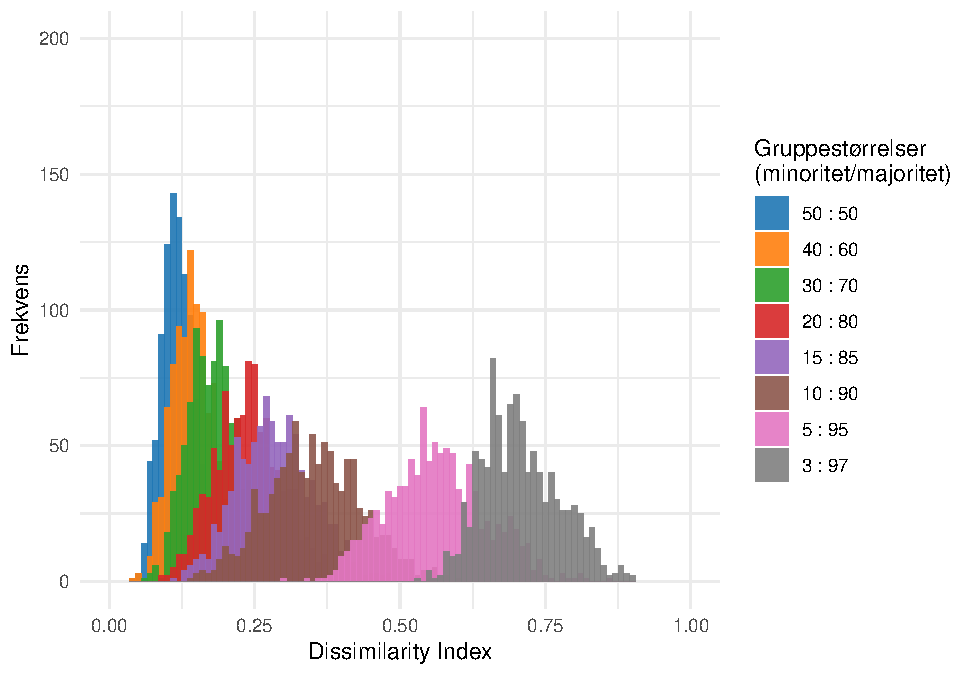
\includegraphics[width=1\linewidth]{en-befolkning-blander-sig_files/figure-latex/fig-9-1-1} \caption{Simuleret fordeling af D index under forskellige relative gruppestørrelser i population på 100 personer}\label{fig:fig-9-1}
\end{figure}

Dette leder til en pointe, der ofte overses i anvendelsen af \(D\). Populationssammensætningsinvarians og indeksets fokus på relativ fordeling---eller ubalance---mellem enheder gør indekset meget følsomt over for størrelsen og antallet af enheder. Denne egenskab kan gøre sammenligninger mellem forskellige kontekster problematiske. For eksempel, hvis det fysiske skolelandskab (antallet og størrelsen af skoler) varierer markant mellem to kommuner, vil forskellen i observeret \(D\) også udtrykke denne strukturelle forskel i skolelandskabet mellem kommunerne. Dette er et velkendt problem i den geografiske forskningslitteratur, kendt som \href{https://en.wikipedia.org/wiki/Modifiable_areal_unit_problem}{``the Modifiable Areal Unit Problem''} (\emph{MAUP}). Relateret hertil er også det klassiske problem i geografiske analyser kendt som ``the small-unit bias,'' hvor det mange steder er vist, at tilfældig fordeling mellem små enheder systematisk kan resultere i høj segregering (\citeproc{ref-carrington1997}{Carrington \& Troske, 1997}).

Opsummeret betyder det, at selvom \(D\)-indekset principielt kan variere fra \(0\) til \(1\) (ingen \(\rightarrow\) komplet segregering), vil ``ingen segregering'' være tæt på umulig at opnå, hvis grupperne varierer markant i størrelse, som vi også ser i Figur \ref{fig:fig-9-1}. Der kan simpelthen være for få minoriteter og for mange enheder til, at deres fordeling mellem enheder kan matche majoritetens fordeling (\citeproc{ref-harris2017}{Harris, 2017}). Som diskuteret i \hyperref[kap3]{kapitel 3} er dette forhold aktuelt i den danske case, hvor andelen af minoriteter, selvom den er stigende, har været og fortsæt er relativt lille i mange kommuner.

\subsection{Korrigeret D-indeks}\label{korrigeret-d-indeks}

En måde at tilgå denne begrænsning, at tilfældige fordelinger også kan producere relativt høje grader af segregering, er blevet præsenteret af Harris (\citeproc{ref-harris2017}{2017}). Blandt Harris' metodiske bidrag til segregeringslitteraturen er en udvidelse af \(D\)-indekset, der korrigerer målet for det gennemsnitlige niveau af segregering under forudsætning af tilfældig fordeling (\href{https://en.wikipedia.org/wiki/Independent_and_identically_distributed_random_variables}{iid}), givet de faktiske gruppestørrelser og enheder. Dette gennemsnit er afledt af simulerede fordelinger af en population mellem enheder, efter samme logik som Figur \ref{fig:fig-9-1}. Denne korrigering af \(D\) tager altså højde for, at selvom segregering måles til at være høj, kunne denne grad af segregering have opstået under tilfældig fordeling af grupperne under de givne strukturelle forhold. Diop \& Larsen (2024) anvender denne korrigering af den målte segregering for at kunne bidrage med en mere nuanceret beskrivelse af segregering på det danske arbejdsmarked i en kontekst med ændrende demografiske forhold over tid (se \hyperref[kap4]{kapitel 4}).

\section{Separationsindekset}\label{separationsindekset}

Hvor sammensætningsinvariansen ofte fremhæves som en attraktiv egenskab ved \(D\), er det dog også en tilbagevendende diskussion i den metodiske litteratur, at det ikke i alle situationer er en attraktiv egenskab ved et segregeringsmål. Særligt ikke hvis vi eksplicit er interesserede i intergruppe-interaktioner. Sammensætningsinvariansen gør nemlig, at \(D\) per definition ikke opfanger ændringer i strukturelle betingelser for intergruppe eksponering på individuelt niveau. Ulige fordeling mellem enheder betyder nemlig ikke nødvendigvis separering mellem grupper (se \hyperref[forskel]{næste sektion}). Med separering menes der fysisk adskillelse af grupperne i hverdagen og ikke blot om en person befinder sig i en enhed, hvor der er højere eller lavere andel af personer fra samme gruppe, relativt til det større område, da det kan indbefatte områder, som fortsat er relativt befolkningsmæssigt heterogene.

For at kunne svare på, om grupperne ikke bare er ulige fordelt mellem enheder, men faktisk separeret i deres daglige liv---det vil sige, at de ikke forventes at mødes tilfældigt en given dag---kræver det en beskrivelse af, om den ulige fordeling er \emph{koncentreret} i få enheder eller \emph{spredt} over flere enheder. Er ulige fordeling koncentreret, betyder det, at de to grupper befinder sig i enheder (skoler, nabolag, arbejdspladser, etc.), som er homogene. Det vil sige, at enten minoriteten eller majoriteten udgør hele eller størstedelen af populationen i hver enhed. Er ulige fordeling modsat spredt, betyder det, at minoritetsgruppen er tyndt spredt mellem nogle af enhederne i området. Dette betyder, at gruppen er ulige fordelt, fordi populationen ikke er lige repræsenteret i alle enheder, men samtidig varierer befolkningssammensætningen kun moderat mellem enheder. Dette er ofte tilfældet, hvis minoriteten er markant mindre end majoriteten og ikke udelukkende repræsenteret i enkelte enheder.

Implikationen er, at hvis ulige fordeling er spredt, vil der stadig være relativt høj gensidig eksponering mellem minoritets- og majoritetsgruppen i forhold til, hvor meget eksponering der strukturelt er muligt, idet minoriteten udgør en relativ lille del af de enheder, hvor de er til stede. I modsætning til ulige fordeling, der er koncentreret, hvor hver gruppe primært er eksponeret for deres egen gruppe. Det vil sige, at grupperne er isolerede og primært kun i kontakt med personer fra deres egen gruppe. I det første tilfælde er grupperne altså ikke separerede da grupperne stadig er eksponerede for hinanden i det omfang, det kan lade sig gøre under de strukturelle forudsætninger givet ved populationssammensætningen og antallet og størrelsen af enheder. \emph{Gruppeseparation} refererer således til en fordeling af to grupper, hvor fordelingen er sådan, at hver gruppe befinder sig i en enhed, hvor deres egen gruppe er disproportionalt koncentreret. Med andre ord er den typiske enhed i et område befolkningsmæssigt homogen. \(D\) kan ikke beskrive denne separation, idet ulige fordeling ikke per definition signalerer disproportional koncentration af grupper---hvilket til tider er en forfejlet opfattelse i empiriske segregeringsstudier (\citeproc{ref-fossett2017}{Fossett, 2017}).

Separering kan i stedet beskrives med \emph{Separationsindekset}\footnote{Et problem gennem segregeringslitteraturen er, at Separationsindekset er kendt under mange navne (\citeproc{ref-fossett2017}{Fossett, 2017}), da metodiske artikler ofte har valgt at give indekset et nyt navn, som de finder mere korrekt. Indekset er derfor også kendt som \emph{The revised index of isolation}, \emph{The correlation ratio} eller \(eta^{2}\), \(r_{ij}\), \emph{The variance ratio} og \emph{The segregation index}.} (\(S\)), som måler forskellen i den parvise majoritets-minoritets eksponering til majoritetsgruppen. Det vil sige at \(S\) måler den vægtede forskel mellem gruppe \(A\)'s eksponering til gruppe \(A\) og gruppe \(B\)'s eksponering til gruppe \(A\). \(S\) er ligesom \(D\) et to-gruppe mål for segregering, som måler den relative grad af segregering mellem to grupper. Men hvor \(D\) udtrykker \emph{fordeling}, udtrykker \(S\) \emph{sandsynlighed for eksponering} mellem to grupper.

Med de samme notationer som i \hyperref[dissimkap]{foregående sektion} kan \(S\) udregnes som

\begin{equation}
\label{eq:sep}
S = \frac{{\textstyle \sum_{i=1}^{k}} n_{i}^{*} \left ( p_{i}-P \right )^{2} }{ TP \left ( 1-P \right ) } 
\end{equation}

Ligesom dissimilaritetsindekset, anvender separationsindekset også \(P\) som grundlag for sammenligning mellem enheder, men bestemmer afvigelsen af hver enkelt enheds gruppesammensætning (\(p_{i}\)) fra \(P\) med andre regler. Hvor \(D\) måler den absolutte afstand mellem \(p_{i}\) og \(P\), er \(S\) givet som den kvadrerede forskel mellem \(p_{i}\) og \(P\) vægtet i forhold til størrelsen af de enkelte enheder, \(n_{i}^{*}\). Målet er endeligt afledt ved at dividere med den maksimalt mulige score i nævneren for at standardisere målet til en \(0-1\) skala (\citeproc{ref-james1985}{James \& Taeuber, 1985}; \citeproc{ref-zoloth1976}{Zoloth, 1976}).

Denne forskel i bestemmelsen af de summerede afvigelser fra ``lige fordeling'' har stor substantiel betydning for, hvad indekset faktisk måler, og tolkningen af segregering, selvom ligning \eqref{eq:sep} på mange måder ligner ligning \eqref{eq:dissim}. Som diskuteret udtrykker \(S\) derfor ikke \emph{(u)lige fordelinger}, men forskellen i parvis skaleret eksponering til majoritetspersoner mellem majoritets- (\(A\)) og minoritetsgruppen (\(B\)). \(S\) måler derfor \emph{sandsynligheder for intergruppeeksponering, korrigeret for den samlede populationssammensætning} (\citeproc{ref-bell1954}{Bell, 1954}; \citeproc{ref-fossett2017}{Fossett, 2017}) udtrykt som en brøkdel af den maksimalt mulige værdi.

Vægtningen af indekset relaterer sig til, at \(S\) er afledt af isolerings- og eksponeringsindeksene (\(P^{*}\)-indeks, se Farley (\citeproc{ref-farley1984}{1984})), som udtrykker sandsynligheden for, at to tilfældigt udvalgte personer i en enhed tilhører samme eller forskellige grupper (\citeproc{ref-gorard2002}{Gorard \& Taylor, 2002}). \emph{Eksponeringsindekse}t, \(_{A}P^{*}_{B}\), udtrykker sandsynligheden for, at en tilfældig person fra \(A\) befinder sig i en enhed med en person fra \(B\). \emph{Isoleringsindekset}, \(_{A}P^{*}_{A}\), udtrykker derimod sandsynligheden for, at en tilfældig person fra \(A\) befinder sig i en enhed med en anden fra \(A\)\footnote{To meget forsimplede antagelser er nødvendige i denne tolkning (\citeproc{ref-bell1954}{Bell, 1954}). For det første antages det, at møder mellem personer foregår inden for den pågældende enhed (skoler, arbejdspladser, nabolag), og for det andet, at hver person i en pågældende enhed har lige sandsynlighed for at møde hver enkelt person inden for enheden. Det er veldokumenteret, at begge antagelser ikke er tilfældet i praksis (\citeproc{ref-mcpherson2001}{McPherson et al., 2001}). \(P^{*}\) skal derfor tolkes som \emph{den minimale sandsynlige eksponering mellem personer fra samme/forskellige grupper}, under antagelse af at den faktiske intragruppe eksponering er højere.}. Begge mål kan tage værdier fra \(0\) til \(1\), og hvis populationen er inddelt i kun to grupper, gælder det, at \(_{A}P^{*}_{B} + _{A}P^{*}_{A} = 1\). Derudover er målene asymmetriske, hvilket betyder, at \(_{A}P^{*}_{B} = _{B}P^{*}_{A}\) kun i tilfælde, hvor \(A\) og \(B\) udgør lige store andele af befolkningssammensætningen, eller \(_{A}P^{*}_{B} \neq _{B}P^{*}_{A}\). Disse mål opfylder derfor ikke sammensætningsinvariansen, men er afhængige af størrelsen på de grupper, der sammenlignes (\citeproc{ref-massey1988}{Douglas S. Massey \& Denton, 1988}), da sandsynligheden for eksponering eller isolering er summen af produktet af to sandsynligheder (se Bell (\citeproc{ref-bell1954}{1954})): (1) sandsynligheden for, at en person fra gruppe \(A\) møder en anden person fra gruppe \(A\): \(\left( n_{i}^{A} - 1 \right) / \left( n_{i}^{B} - 1 \right)\), og (2) sandsynligheden for, at en tilfældig person fra gruppe \(A\) befinder sig i den pågældende enhed, \(i\): \(n_{i}^{A} / N^{A}\). Et produkt, der kan udtrykkes algebraisk som: \(P^{*}=\frac{1}{A} {\textstyle \sum_{i=1}^{k}\frac{n_{i}^{A \space 2}}{n_{i}^{B}}}\). Sandsynligheden for intergruppeeksponering---eller relativ isolation---tager altså afsæt i befolkningssammensætningen.

Problemet ved at anvende \(P^{*}\) ukorrigeret i bestemmelsen af den relative isolation af grupperne, som diskuteret af Bell (\citeproc{ref-bell1954}{1954}), er, at den mindste værdi \(P^{*}\) kan tage, er den heterogene blanding af gruppe \(A\) i et pågældende område, givet som \(N^{A}/N^{B}\). Derfor gælder det også, at sandsynligheden for intragruppeeksponering i gruppe \(A\) er større end i gruppe \(B\), hvis gruppe \(A\) udgør en større andel af populationen, \emph{selv hvis populationen er ligeligt fordelt mellem enheder}. Hvis der ikke korrigeres for populationsstørrelser (\(T=N^{A}+N^{B}\)), kan komparative beskrivelser af forventet eksponering, givet alene som \(P^{*}\), mellem områder derfor være delvist vildledende i en substantiel tolkning. For eksempel, hvis vi forestiller os to kommuner: den ene kommune (\(X\)) består af \(30\%\) personer fra gruppe \(B\), mens den anden kommune (\(Y\)) består af \(2\%\) personer fra gruppe \(B\). Selv hvis minoritetsgruppen var ligeligt fordelt mellem alle enheder i hver kommune, således at alle enheder har den samme andel---altså ingen segregering i henhold til \(D\)---vil det i kommune \(X\) gælde, at \(P^{*}=0.3\), mens det i kommune \(Y\) gælder at \(P^{*}=0.02\). Med disse ``rå'' mål for eksponering er høje/lave grader af eksponering ikke nødvendigvis et udtryk for segregering, men kan blot reflektere, at der er flere personer fra gruppe \(B\) i den ene kommune sammenlignet med den anden. Med andre ord, med \(D\) ser vi ingen forskelle i segregeringsniveau mellem \(X\) og \(Y\), selvom der tydeligvis er substantielle forskelle i graden af intergruppeeksponering, mens vi med \(P^{*}\) kan ende med en beskrivelse, der grundlæggende ikke siger andet end ``der er flere minoriteter i \(X\) end i \(Y\)''---en forskel, der ikke nødvendigvis udtrykker en forskel i segregeringsprocesser mellem kommunerne, kun potentialet for omfanget af segregering (se \ref{fig:fig-9-1}).

\(S\) imødegår disse begrænsninger. Forskellen på \(P^{*}\) og \(S\) er, at \(S\) er en standardisering---eller normalisering---af \(P^{*}\)-målene, der kontrollerer for befolkningssammensætningen og samtidig eliminerer asymmetrien i målene. Ved at normalisere med hensyn til størrelsen på enhederne (\(n_{i}^{*}\)) og den maksimalt mulige eksponering/isolering (\(TP(P-1)\)) udledes et mål, hvor den ekstreme minimumsværdi \(0\) repræsenterer en situation, hvor den sandsynlige eksponering mellem grupperne er lig \emph{den hypotetiske sandsynlige eksponering, hvis gruppe \(A\) var lige fordelt mellem enheder}. Den ekstreme maksimumsværdi \(1\) opnås i situationer, hvor sandsynligheden for tilfældig eksponering mellem gruppe \(A\)-medlemmer i en given enhed er \(100\%\). \(S\) er altså udtrykt som en brøkdel af den maksimalt mulige eksponering.

Denne korrigering for befolkningssammensætning har den implikation, at segregeringsmålets forventede spænd mellem minimum og maksimum ikke på samme måde er følsomt overfor relative gruppestørrelser (se Figur \ref{fig:fig-9-2}). \(S\) forventede spænd er dog strukturelt påvirket af antallet af enheder, som en population kan blive sorteret mellem (se Figur \ref{fig:fig-9-3}). Som Fossett (\citeproc{ref-fossett2017}{2017}) har demonstreret, indeholder \(S\), i kombination med mål for fordeling såsom \(D\), dermed information om, hvorvidt ulige fordeling er koncentreret eller spredt---hvis \(S\) er lavt, mens \(D\) er højt, vil den ulige fordeling være karakteriseret som spredt, mens et højt \(S\) og højt \(D\) indikerer en koncentreret ulige fordeling. Som Fossett skriver, \(S\) \emph{``therefore serves as an indication of `prototypical segregation,' implying actual separation between groups rather than the mere uneven distribution of a minority group''} (s. 96).

\begin{figure}
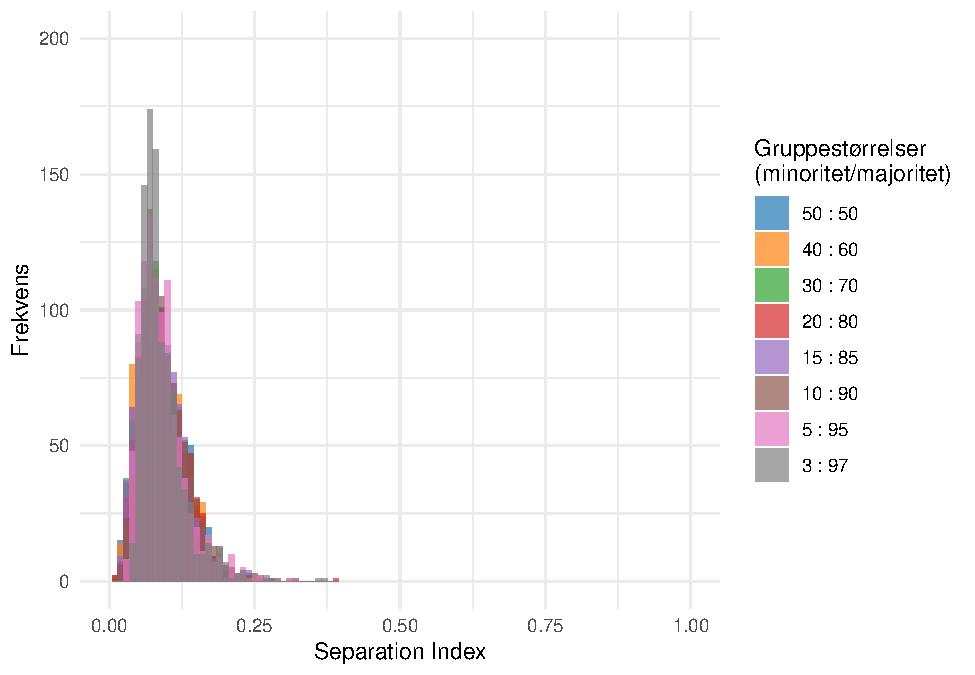
\includegraphics[width=1\linewidth]{en-befolkning-blander-sig_files/figure-latex/fig-9-2-1} \caption{Simuleret fordeling af S index under forskellige relative gruppestørrelser i population på 100 personer (10 enheder).}\label{fig:fig-9-2}
\end{figure}

\begin{figure}
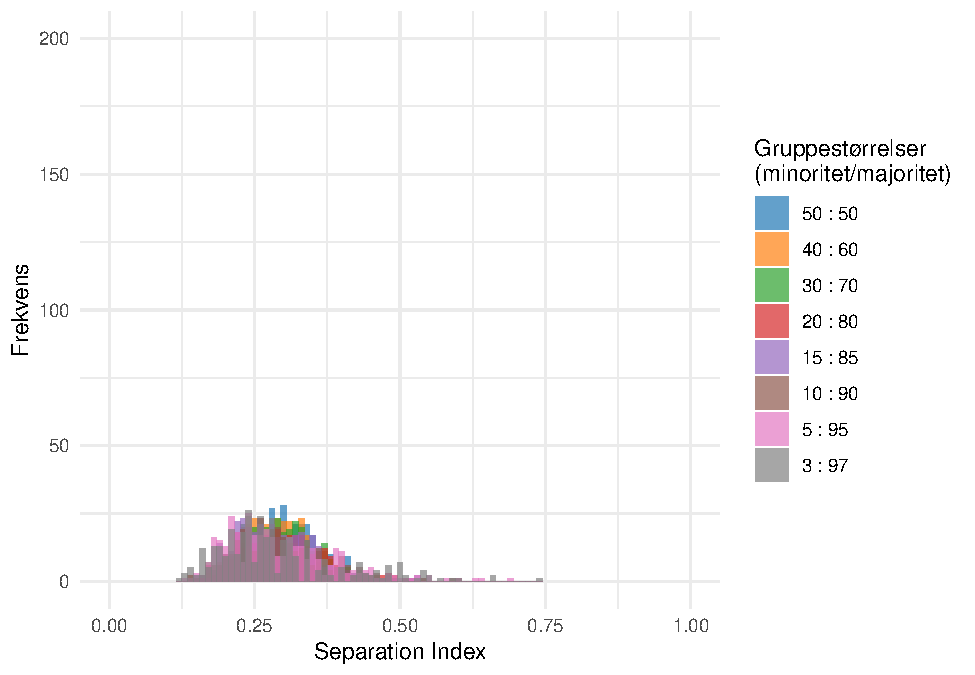
\includegraphics[width=1\linewidth]{en-befolkning-blander-sig_files/figure-latex/fig-9-3-1} \caption{Simuleret fordeling af S index under forskellige relative gruppestørrelser i population på 100 personer (30 enheder).}\label{fig:fig-9-3}
\end{figure}

\section{Sammenhæng mellem S og D}\label{forskel}

I praksis ser vi ofte, at \(S\) og \(D\) korrelerer, men graden af korrelation kan variere betydeligt mellem områder, fordi \(D\) ikke per definition signalerer polarisering og koncentreret fordeling mellem grupper. \(S\) og \(D\) kan have samme score, men kun i tilfælde hvor begge mål er \(1\), hvilket udtrykker en situation, hvor begge grupper befinder sig i homogene enheder, hvor de udgør \(100\%\). Altså, når koncentrationen mellem enheder i et område er ved deres maksimum, vil \(S=D\). Når \(S\) og \(D\) er identiske eller tilnærmelsesvis af samme størrelsesorden---lav-lav, medium-medium, eller høj-høj-scores---er segregering derfor karakteriseret som det, Fossett (\citeproc{ref-fossett2017}{2017}) kalder ``prototypisk segregering.'' Når \(S\) og \(D\) derimod divergerer med en høj \(D\)-score men lav \(S\)-score, er fordelingen af majoriteter og minoriteter mellem enheder karakteriseret som en ``ulige men spredt fordeling''. Det vil sige, at selvom minoritetsgruppen ikke er repræsenteret i alle enheder i et givent område, udgør de fortsat en numerisk minoritet i de enheder, hvor de er repræsenteret. Minoritetsgruppen er simpelthen for lille---eller for ``tyndt spredt''---til at kunne udgøre numerisk overtal i nogen af enhederne i et område. Selvom \(D\) i sådanne situationer vil være relativt højt, er det en strukturel betingelse givet af den relative størrelse af grupperne og antallet af enheder (se Figur \ref{fig:fig-9-1}), og ikke nødvendigvis produktet af segregeringsprocesser. Disse forhold er indfanget af \(S\), som i denne situation vil være lav og afvige relativt meget fra \(D\), fordi \(S\) kun tager høje værdier, når enhederne i et område er homogene. Dette er ikke muligt rent strukturelt, hvis minoritetsgruppen er markant mindre end majoritetsgruppen, og kun forventeligt i områder, hvor grupperne nærmer sig relativt lige andele af populationen. I absolutte værdier kan \(S\) derfor heller ikke være større end \(D\). Derfor er tommelfingerreglen, at når grupper varierer meget i relative størrelser og/eller antallet af enheder er højt, kan \(S\) strukturelt være nævneværdigt lavere end \(D\) (se Figur \ref{fig:fig-9-2} og Figur \ref{fig:fig-9-3}). Se Figur \ref{fig:fig-9-4} for stiliserede beskrivelser af de tre mulige idealtypiske kombinationer af \(S\) og \(D\).

\begin{figure}
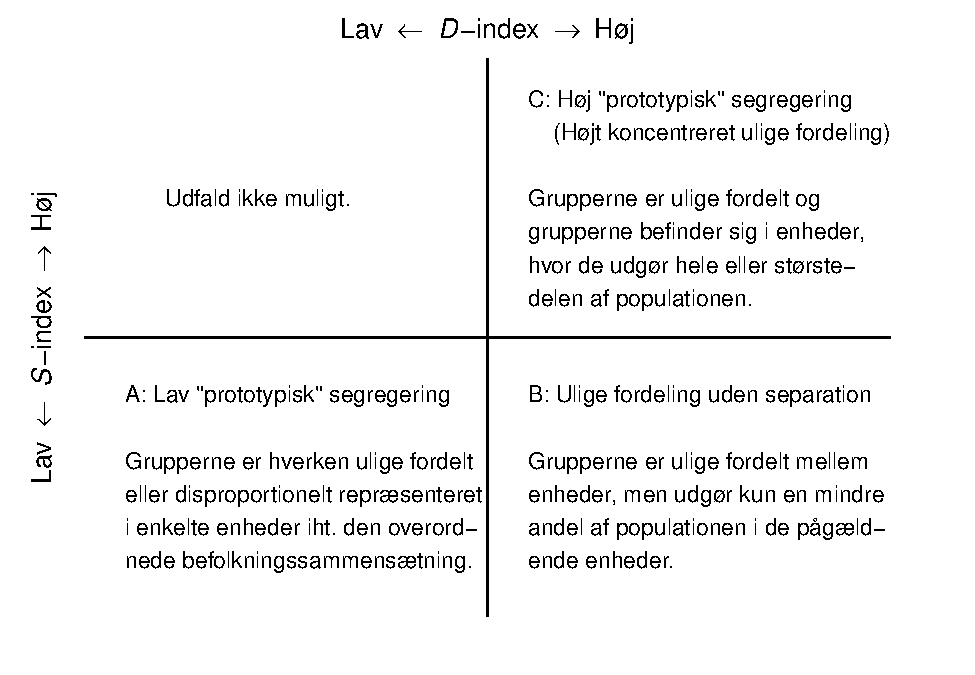
\includegraphics[width=1\linewidth]{en-befolkning-blander-sig_files/figure-latex/fig-9-4-1} \caption{Mulige kombinationer af (absolutte) S-D værdier efter Fossett (2017, s. 85).}\label{fig:fig-9-4}
\end{figure}

En anden teknisk forskel mellem de to mål er, at \(S\) er mere sensitivt end \(D\), fordi \(S\) opfanger et helt spektrum af eksponering mellem grupper, mens \(D\) kun opfanger, hvor mange der befinder sig i enheder, som er binært grupperet som under/over paritet. Det vil sige, at i \(D\), ligning \eqref{eq:dissim}, gør det ingen forskel, hvor langt fra paritet en given enhed er. Det gør det modsat i \(S\), ligning \eqref{eq:sep}. Ved et segregeringsreducerende flyt, forstået som et flyt til en enhed med relativt lavere andel af personer fra egen gruppe, eller et segregeringsøgende flyt, forstået som et flyt til en enhed med en relativt større andel af personer fra egen gruppe, vil \(S\)-indekset reagere ``stærkere'' (ændre sig mere) for flyt mellem to homogene enheder---hvor den ene har en andel minoriteter på \(100\%\) og den anden en andel på \(0\%\)---end flyt mellem områder, som er relativt blandede, selvom de to enheder formelt er over og under paritet (for eksempel, hvor den ene enhed har en andel på \(49\%\) og den anden en andel på \(51\%\)). \(D\) vil modsat opfange disse to flyt med identisk påvirkning på den målte grad af segregering (se Fossett (\citeproc{ref-fossett2017}{2017}, s. 90--96) for teknisk forklaring og eksempler). Det betyder altså også, at der vil være flytninger, som kun bliver registreret i \(S\), der registrerer alle ændringer, men ikke i \(D\), hvis flytningen er mellem to enheder, der selvom de har forskellig befolkningssammensætning, men begge enheder er over/under paritet i forhold til det større områdes befolkningssammensætning. Dette gør sig særligt relevant på store skalaer, såsom national skala, hvor flytninger indenfor kommuner med relativt høje eller lave andele af minoriteter ikke registreres som ændringer i \(D\), selvom disse flyt kan påvirke graden af eksponering/isolering mellem minoriteter og majoriteter. Derfor ses det også empirisk, at der kan være situationer, hvor \(D\)-indekset giver en indikation af faldende segregering, mens \(S\) vil vise det modsatte. Det er for eksempel tilfældet ved udviklingen i skolesegregering på national skala (se Figur \ref{fig:fig-3-2}).

\chapter{Andet bilag\ldots{}}\label{bilag2}

Bilag B, hvis der er et \ldots{}

\end{document}
